\documentclass[a4paper,12pt,twoside]{article}
\usepackage[left=1in,right=1in,top=1in,bottom=1in]{geometry}

\usepackage{xeCJK}
\setCJKmainfont{Songti TC}
\setCJKfamilyfont{kai}{Songti TC}
\newcommand{\kai}{\CJKfamily{kai}} % 用 \kai{使用楷書}

\usepackage{lmodern}
\usepackage{titling}
\usepackage{titlesec}
\usepackage{graphicx}
\usepackage{float}
\usepackage{amsmath, amsthm, amssymb, amsfonts, mathrsfs}
\usepackage{upgreek} % 直立的希臘字母

\usepackage[shortlabels]{enumitem}
\usepackage{setspace}
\renewcommand{\baselinestretch}{1.5}
\usepackage[colorlinks]{hyperref}
\usepackage{fancyvrb}
\usepackage{fancyhdr}
\usepackage{multicol}
\usepackage{caption}
\usepackage{listings}
\usepackage{bm}
\usepackage{bbm} % for \mathbbm{1} (indicator function)
\usepackage{centernot}
\usepackage{mdframed}
\usepackage{tikz}
\usetikzlibrary{patterns, arrows.meta, positioning}
\usepackage[nameinlink, capitalise]{cleveref}
\usepackage{diagbox}
\usepackage{booktabs}
\usepackage{multirow,array}
\usepackage{tabularx}
\usepackage{mathtools}
\usepackage{indentfirst} % 首段 indent
\setlength{\parindent}{2em}
\usepackage{cancel} % 數學式子畫線槓掉
\newcommand\mcancel[2][red]{\setbox0=\hbox{$#2$}%
\rlap{\raisebox{.45\ht0}{\textcolor{#1}{\rule{\wd0}{1pt}}}}#2}
\usepackage{datetime2}

\AtBeginDocument{%
 \setlength{\abovedisplayskip}{6pt}
 \setlength{\belowdisplayskip}{6pt}
 \setlength{\abovedisplayshortskip}{4pt}
 \setlength{\belowdisplayshortskip}{4pt}
}

\definecolor{codegreen}{rgb}{0,0.6,0}
\definecolor{codegray}{rgb}{0.5,0.5,0.5}
\definecolor{codepurple}{rgb}{0.58,0,0.82}
\definecolor{backcolour}{rgb}{0.95,0.95,0.92}

\lstdefinestyle{mystyle}{
 backgroundcolor=\color{backcolour},
 commentstyle=\color{codegreen},
 keywordstyle=\color{magenta},
 numberstyle=\tiny\color{codegray},
 stringstyle=\color{codepurple},
 basicstyle=\ttfamily\footnotesize,
 breakatwhitespace=false,
 breaklines=true,
 captionpos=b,
 keepspaces=true,
 numbers=left,
 numbersep=5pt,
 showspaces=false,
 showstringspaces=false,
 showtabs=false,
 tabsize=2
}
\lstset{style=mystyle}

\hypersetup{citecolor=blue, linkcolor=blue, urlcolor=blue}

\DeclareMathOperator{\supp}{supp}
\DeclareMathOperator{\skewness}{Skewness}
\DeclareMathOperator{\DU}{D-U}
\DeclareMathOperator{\CU}{C-U}
\DeclareMathOperator{\Geo}{Geo}
\DeclareMathOperator{\Pois}{Pois}
\DeclareMathOperator{\Gam}{Gam}
\DeclareMathOperator{\LN}{LogN}
\DeclareMathOperator{\cov}{Cov}
\DeclareMathOperator*{\argmax}{arg\,max}
\DeclareMathOperator*{\argmin}{arg\,min}
\DeclareMathOperator{\re}{Re}
\DeclareMathOperator{\im}{Im}

\newcommand{\N}{\mathbb{N}}
\newcommand{\Z}{\mathbb{Z}}
\newcommand{\Q}{\mathbb{Q}}
\newcommand{\R}{\mathbb{R}}
\newcommand{\C}{\mathbb{C}}
\newcommand{\G}{\mathcal{G}}
\newcommand{\mP}{\mathbb{P}}
\newcommand{\F}{\mathcal{F}}
\newcommand{\B}{\mathcal{B}}
\newcommand{\1}{\mathbbm{1}}
\newcommand{\Poi}{\text{Poi}}
\newcommand{\Var}{\text{Var}}
\newcommand{\as}{\text{a.s.}}
\newcommand{\vect}[1]{\boldsymbol{\mathbf{#1}}}
\newcommand{\paren}[1]{\left({#1}\right)}
\newcommand{\brk}[1]{\left[{#1}\right]}
\newcommand{\curl}[1]{\left\{{#1}\right\}}
\renewcommand{\lambda}{\lambdaup}

\theoremstyle{definition} % 定理環境 style 改用正體
\newtheorem{theorem}{定理}
\newtheorem{definition}{定義}
\newtheorem*{definition*}{定義}
\newtheorem{example}{例子}
\newtheorem{exercise}{練習}
\newtheorem{corollary}{推論}
\newtheorem{property}{性質}
\newtheorem{prop}{命題}
\newtheorem{lemma}{引理}
\newtheorem{problem}{問題}
\newtheorem*{remark}{註}

\renewcommand{\figurename}{圖}
\renewcommand{\tablename}{表}

\DeclareMathOperator{\var}{Var}
\DeclareMathOperator{\corr}{corr}
\DeclareMathOperator{\rank}{rank}
\DeclareMathOperator{\MSE}{MSE}
\DeclareMathOperator{\SSE}{SSE}
\DeclareMathOperator{\SST}{SST}
\DeclareMathOperator{\SSR}{SSR}
\DeclareMathOperator{\sgn}{sign}
\DeclareMathOperator{\alt}{Alt}
\DeclareMathOperator{\adj}{adj}
\DeclareMathOperator{\curlOp}{curl}
\DeclareMathOperator{\spn}{span}
\DeclareMathOperator{\sse}{SSE}
\DeclareMathOperator{\tr}{tr}

\newcommand{\ep}{\varepsilon}
\newcommand{\p}{\partial}
\newcommand{\abs}[1]{\left|#1\right|}
\newcommand\norm[1]{\left\lVert#1\right\rVert}
\newcommand{\innerprod}[1]{\langle#1\rangle}
\newcommand{\ds}{\displaystyle}
\newcommand{\blank}{\rule[-1mm]{1.5cm}{0.1mm}}
\newcommand{\dint}{\displaystyle\int}
\renewcommand{\bar}{\overline}

\newtheoremstyle{remark}{}{}{}{}{\bfseries\sffamily}{.}{.5em}{#1}
\theoremstyle{remark}

\newtheorem*{remark*}{\textit{Remark}}
\newtheorem*{solution*}{解}

\AtEndEnvironment{solution*}{\hfill$\square$}
\newtheorem*{hint*}{Hint}


\newcommand{\redtext}[1]{{\color{red} #1}}
\newcommand{\bluetext}[1]{{\color{blue} #1}}

\fancypagestyle{firstpage}{
  \fancyhf{}
  \fancyhead[R]{\small《高中數學實驗教材》第 3 冊（自然組）}
  \fancyhead[L]{\small 第 4 章\quad 座標幾何}
  \fancyfoot[C]{\thepage}
}

\pagestyle{fancy}
\setlength{\headheight}{14pt}
\renewcommand{\headrulewidth}{0.5pt}
\renewcommand{\footrulewidth}{0pt}
\fancyhead{}
\fancyhead[LE]{\small 《高中數學實驗教材》第三冊（自然組）}
\fancyhead[RO]{\small 第四章\quad 座標幾何}
\fancyfoot[C]{\thepage}

\title{\LARGE\textbf{《高中數學實驗教材》第三冊（自然組）}\\[0.5em] \Large\textbf{第四章\quad 座標幾何}}
\author{\textbf{高中數學實驗教材編輯小組}\quad 編著}
\date{民國六十四年（1975）再版}

\begin{document}

\maketitle
\thispagestyle{firstpage}

% ==========================================
% 掃描檔勘誤、文字校訂與疑難處說明（依規則整理於目錄之前）
% ==========================================
\section*{【說明】第四章掃描檔勘誤、疑難處與文義校訂表}
\addcontentsline{toc}{section}{【說明】第四章掃描檔勘誤、疑難處與文義校訂表}
\label{sec:errata_notes_b3_ch4}

本章依據 1975 年再版《高中數學實驗教材 第三冊（自然組）》（高二上）第四章「座標幾何」掃描原件完整轉錄為 \LaTeX{} 格式。為忠實反映教材原始內容並兼顧排版品質與嚴謹性，依作業規範將掃描檔中出現之印刷訛誤、符號缺漏、字模損毀、歷史印記雜訊及文義疑難處詳細考證彙整於下表。讀者可點擊表格中之章節連結直接跳至正文對應位置：

\begin{table}[H]
\centering
\small
\renewcommand{\arraystretch}{1.35}
\begin{tabularx}{\textwidth}{|p{3.2cm}|p{3.8cm}|X|}
\hline
\textbf{章節位置} & \textbf{掃描檔原始現象 / 誤植} & \textbf{考證說明與校訂處理} \\ \hline

\hyperref[note:b3-ch4-p132-tilde-pronounce]{§ 4-1 頁 132 英文波浪號拼寫} & 
「〔“$\sim$”讀音如 tilda〕」 & 
英文波浪號常用拼寫為 tilde。正文忠實保留原刊字樣並加註說明。 \\ \hline

\hyperref[note:b3-ch4-p136-fig4-4-a-scale]{§ 4-1 頁 136 圖 4-4-a 刻度比例} & 
圖 4-4-a 印作「$|\tilde{\mathbf{e}}_1|=2, |\tilde{\mathbf{e}}_2|=4$」 & 
下文行文說明作「$|\tilde{\mathbf{e}}_1|=1, |\tilde{\mathbf{e}}_2|=2$」，相差二倍刻度。正文忠實保留原文對比並備註。 \\ \hline

\hyperref[note:b3-ch4-p177-l1-l2-subscripts]{§ 4-4 頁 177 論例 5 下標漏印} & 
常數項均印作「$+c$」 & 
解文中代入明確為「$+c_1$」與「$+c_2$」。正文校訂補齊下標並註記。 \\ \hline

\hyperref[note:b3-ch4-p193-formula-ref]{§ 4-6 頁 193 公式編號指涉} & 
「若 $L$ 可寫成 (1) 式...」 & 
此處實指上一頁之共點直線系方程式 (36)。正文予以校訂並加註。 \\ \hline

\hyperref[note:b3-ch4-p203-ceva-ref]{§ 4-7 頁 203 命題 3 公式引用} & 
「(31) 式成立，亦卽...」 & 
原書印作 (31) 式，實指本節西瓦定理之式 (40)。正文予以校訂並備註。 \\ \hline

\hyperref[note:b3-ch4-p207-theorem-ref]{§ 4-7 頁 207 內心證明定理引用} & 
「由本節定理 6，知...」 & 
三線共點行列式條件實為 § 4-5 定理 2（定理 6 為西瓦定理）。正文保留原字樣並註記。 \\ \hline

\hyperref[note:b3-ch4-p213-equation-ref]{§ 4-8 頁 213 公式編號缺字} & 
「當我們遇到 (4) 式這樣...」 & 
第二個數字漏印，實指三元一次平面方程 (44)（或式 (47)）。正文予以校訂並加註。 \\ \hline

\hyperref[note:b3-ch4-p221-subscript-typo]{§ 4-8 頁 221 第 8 題下標誤植} & 
比例式分子印作「$y - y_5$」 & 
此處實為「$y - y_0$」。正文予以校訂並註記。 \\ \hline
\end{tabularx}
\caption{第四章掃描檔勘誤、疑難處與文義校訂表}
\label{tab:errata_b3_ch4}
\end{table}

\vspace{1em}
\hrule
\vspace{1em}

\tableofcontents
\newpage

\section{座標幾何}
\label{sec:b3_ch4}

\subsection*{大綱}

\begin{itemize}[leftmargin=2em]
  \item[§ 4-1] \textbf{方程式與軌跡}
  \begin{itemize}[leftmargin=2em]
    \item[甲、] 一般座標系
    \item[乙、] 軌跡
    \item[丙、] 直線的一般方程式表示
  \end{itemize}
  \item[§ 4-2] \textbf{直線的參數式及座標兩點式}
  \begin{itemize}[leftmargin=2em]
    \item[甲、] 參數式
    \item[乙、] 直線的各種代數表示式
    \item[丙、] 直線的斜截式
    \item[丁、] 直線的點斜式
  \end{itemize}
  \item[* § 4-3] \textbf{直線的一般方程}
  \item[§ 4-4] \textbf{法線式及其應用}
  \begin{itemize}[leftmargin=2em]
    \item[甲、] 法線式
    \item[乙、] 直線方向及直線交角
    \item[丙、] 二元一次二式聯立方程求解的幾何解釋
    \item[丁、] 點與直線間距
    \item[戊、] 應用——等溫線；線性規劃
  \end{itemize}
  \item[§ 4-5] \textbf{三線共點條件與二元一次多式聯立方程式}
  \begin{itemize}[leftmargin=2em]
    \item[甲、] 三線共點的條件
    \item[乙、] 二元一次多式聯立方程
  \end{itemize}
  \item[* § 4-6] \textbf{直線系與自由度}
  \begin{itemize}[leftmargin=2em]
    \item[甲、] 共點直線系
    \item[乙、] 自由度
  \end{itemize}
  \item[$\ddagger$ § 4-7] \textbf{座標幾何與向量幾何混合處理的典型與例子}
  \begin{itemize}[leftmargin=2em]
    \item[甲、] 重心的物理意義
    \item[乙、] 西瓦共點定理
    \item[丙、] 三角形諸心定理
  \end{itemize}
  \item[$\ddagger$ § 4-8] \textbf{空間的線性座標幾何}
  \begin{itemize}[leftmargin=2em]
    \item[甲、] 平面的法線式及其一般方程表示
    \item[乙、] 平面上三線共點的幾何解釋
  \end{itemize}
\end{itemize}

\begin{center}
  * \qquad * \qquad *
\end{center}

在第一章裏，我們講過：實際生活上所出現的問題有時本身就是幾何問題，有時可以表成幾何圖形來幫助分析、瞭解與推想。但只依賴幾何常使問題陷入個別處理，不能求得全面發展。若將幾何有系統地轉化成代數，則可用代數的運算來代替幾何上純視覺的推想。上一章所介紹的向量幾何就是一種這樣的轉化，本章我們要討論笛卡兒創始的座標幾何（古稱解析幾何）。這其實是最早出現的有系統的轉化過程。

本章其實已參用了上章引入的向量的語言，到第七節更是揉合向量的好處在處理三角形諸心問題。

在 § 4-1 中，我們先用座標將幾何圖形與其相應的方程式作一對照。要交代的是本章中通常採用一般座標系，而不特定為直角（或正交）座標系，這樣的一般化使我們有較大的自由去選擇座標系，很能簡化一些計算，這個優點到 § 4-7 時將會顯現。

§ 4-2 則將一些直線的幾何量（如斜率、截距、面積、交會、平行或垂直）或性質轉化為其代數方程中一些係數的關係。因此導出各種表示式，如常用的斜截式、兩點式等。

§ 4-3 有系統地把平面上的直線與二元一次方程式的一般對應建立起來。

§ 4-4 採用正交座標系，利用內積，引出直線另一重要表示式：法線式。從這一式子引出交角、距離等幾何量所相應的代數表示。同時，我們將第一冊講過的二元一次聯立方程的求解問題，作一幾何的解釋。在本節末尾，我們談到有實際應用價值的所謂「線性規劃」。

§ 4-5～§ 4-6 把直線共點的條件與二元一次多式聯立方程作一對照。並順此討論直線系及一個一般的概念：“自由度”。

§ 4-7 開始利用到現在引述過的向量幾何與座標幾何，混合來處理古典的平面幾何問題。這樣的處理時常會有稍嫌繁雜的計算。但它有一定的脈絡，抓到這脈絡便有把握處理各色各樣的幾何問題。換句話說，這樣的處理不像直觀幾何所用的劃補助線的方法須要記憶且帶有投機性。

求交點的問題便是求聯立方程的問題，但老是要解這樣的聯立方程有時稍為麻煩，常常向量的處理可以簡化這種計算。

本節是藉西瓦定理及論例 7 來表現這混合處理的一個典型；就是說：注重證明的過程以求掌握一般問題的方法比西瓦定理本身重要。這樣的混合處理，在第五章中還要強調。

§ 4-8 討論空間中的平面方程式。

\subsection{方程式與軌跡}
\label{sec:4-1}

\subsubsection*{甲、一般座標系}

到目前為止，我們都採用直角座標系 $(O; X, Y)$。現在起我們考慮較一般的座標系，這樣的考慮使我們在處理問題時有較大的自由去選取座標，這個優點在 § 4-7 中將會顯現。

在平面上任取不共線三點 $O, \tilde{E}_1, \tilde{E}_2$，考慮兩向量
\[ \tilde{\mathbf{e}}_1 = \vec{O\tilde{E}_1}, \quad \tilde{\mathbf{e}}_2 = \vec{O\tilde{E}_2} \]
〔“$\sim$”讀音如 tilda〕\phantomsection\label{note:b3-ch4-p132-tilde-pronounce}\footnote{【校訂註】原書印作「〔“$\sim$”讀音如 tilda〕」，英文波浪號通常拼作 tilde。正文忠實保留原刊字樣。}

\begin{figure}[H]
\centering
\begin{tikzpicture}[>=Stealth, scale=1.1]
  \coordinate (O) at (0,0);
  \coordinate (Xdir) at (4.5,0);
  \coordinate (Ydir) at (60:4.0);
  \draw[->, thick] (-1,0) -- (5,0) node[right] {$X$};
  \draw[->, thick] (240:0.8) -- (60:4.2) node[above] {$Y$};
  \node[below left] at (O) {$O$};
  
  \coordinate (E1) at (1.8,0);
  \coordinate (E2) at ($(O)+(60:1.6)$);
  \draw[->, very thick, blue!80!black] (O) -- (E1) node[below] {$\tilde{\mathbf{e}}_1$};
  \draw[->, very thick, blue!80!black] (O) -- (E2) node[above left] {$\tilde{\mathbf{e}}_2$};
  \node[above] at (E1) {$\tilde{E}_1$};
  \node[above right] at (E2) {$\tilde{E}_2$};
  
  \coordinate (P) at (3.5, 2.5);
  % P_1 is intersection of line through P parallel to OE_2 with X-axis (line OE_1)
  % P = P_1 + y * (cos 60, sin 60) -> y = P.y / sin 60
  % P_1 = P.x - y * cos 60
  \pgfmathsetmacro{\Py}{2.5}
  \pgfmathsetmacro{\Px}{3.5}
  \pgfmathsetmacro{\yval}{\Py / sin(60)}
  \pgfmathsetmacro{\xval}{\Px - \yval * cos(60)}
  \coordinate (P1) at (\xval, 0);
  \coordinate (P2) at ($(O)+(60:\yval)$);
  
  \draw[dashed, thick] (P) -- (P1);
  \draw[dashed, thick] (P) -- (P2);
  \draw[->, thick] (O) -- (P);
  \fill (P) circle (1.8pt) node[above right] {$P(x,y)$};
  \fill (P1) circle (1.5pt) node[below] {$P_1$};
  \fill (P2) circle (1.5pt) node[left] {$P_2$};
\end{tikzpicture}
\caption{一般座標系}
\label{fig:4-1}
\end{figure}

則平面上任一點 $P$ 皆可根據下面方法得一座標表示，過 $P$ 作直線 $PP_1$ 平行於 $O\tilde{E}_2$，交 $O\tilde{E}_1$ 於 $P_1$，則
\[ \vec{OP} = \vec{OP}_1 + \vec{P_1 P} \]
但 $\vec{OP}_1 \parallel \tilde{\mathbf{e}}_1, \vec{P_1 P} \parallel \tilde{\mathbf{e}}_2$ 故 $\vec{OP}_1, \vec{P_1 P}$ 分別為 $\tilde{\mathbf{e}}_1, \tilde{\mathbf{e}}_2$ 的實倍數（可正可負），即
\[ \begin{aligned}
\vec{OP}_1 &= x\tilde{\mathbf{e}}_1 \\
\vec{P_1 P} &= \vec{OP}_2 = y\tilde{\mathbf{e}}_2
\end{aligned} \]
\[ \vec{OP} = x\tilde{\mathbf{e}}_1 + y\tilde{\mathbf{e}}_2 \]
其中 $x, y$ 表示相應的實倍數。我們稱 $(x, y)$ 為 $P$ 點相關於座標系 $(O; \tilde{\mathbf{e}}_1, \tilde{\mathbf{e}}_2)$ 的座標，或根據座標系 $(O; \tilde{\mathbf{e}}_1, \tilde{\mathbf{e}}_2)$ 所作成的 $P$ 點的座標，常簡記成 $P(x, y)$。

平面上的一個向量 $\mathbf{a}$，唯一地對應一個自 $O$ 出發的有向線段 $\vec{OP}$，我們用端點 $P$ 的座標 $(x, y)$ 來描寫向量 $\mathbf{a}$，亦稱 $(x, y)$ 為向量 $\mathbf{a}$ 相關於座標系 $(O; \tilde{\mathbf{e}}_1, \tilde{\mathbf{e}}_2)$ 的座標，或根據座標系 $(O; \tilde{\mathbf{e}}_1, \tilde{\mathbf{e}}_2)$ 所作成的向量 $\mathbf{a}$ 的座標，常記以
\[ \mathbf{a} = \vec{OP} = x\tilde{\mathbf{e}}_1 + y\tilde{\mathbf{e}}_2 = (x, y) \]
沿 $O\tilde{E}_1, O\tilde{E}_2$ 分別向兩端延伸，得 $X, Y$ 兩軸。〔注意 $x$ 與 $y$ 的絕對值並不一定是 $\overline{OP_1}, \overline{OP_2}$ 的長，因 $\tilde{\mathbf{e}}_1, \tilde{\mathbf{e}}_2$ 並不一定是單位長。〕

特殊地，當 $\bar{\mathbf{e}}_1, \bar{\mathbf{e}}_2$ 為相互垂直的單位向量 $\bar{\mathbf{e}}_1, \bar{\mathbf{e}}_2$ 時，由原點 $O$ 與 $\bar{\mathbf{e}}_1 = \vec{O\bar{E}_1}, \bar{\mathbf{e}}_2 = \vec{O\bar{E}_2}$ 所構成的座標系 $(O; \bar{\mathbf{e}}_1, \bar{\mathbf{e}}_2)$ 稱為正交座標系。正交座標系其實就是本章以前常用的直角座標系。

\begin{example}[例 1]
有兩向量 $\tilde{\mathbf{e}}_1, \tilde{\mathbf{e}}_2$ 它們根據一已給正交座標系 $(O; \mathbf{e}_1, \mathbf{e}_2)$ 所作成的座標分別為 $\tilde{\mathbf{e}}_1 = \vec{O\tilde{E}_1} = (0, -1), \tilde{\mathbf{e}}_2 = \vec{O\tilde{E}_2} = (1, 1)$。$O, \tilde{E}_1, \tilde{E}_2$ 三點不共線，故 $(O; \tilde{\mathbf{e}}_1, \tilde{\mathbf{e}}_2)$ 構成一座標系。

今相關於 $(O; \mathbf{e}_1, \mathbf{e}_2)$ 有四點 $A(2, 1), B(-1, 1), C(-1, 0), D(2, 5)$，問這些點相關於新座標系 $(O; \tilde{\mathbf{e}}_1, \tilde{\mathbf{e}}_2)$ 之座標為何？又 $\tilde{\mathbf{e}}_1, \tilde{\mathbf{e}}_2$ 相關於 $(O; \tilde{\mathbf{e}}_1, \tilde{\mathbf{e}}_2)$ 本身之座標為何？
\end{example}

\begin{figure}[H]
\centering
\begin{tikzpicture}[scale=0.75]
  % Grid
  \draw[step=0.5, gray!40, very thin] (-6,-6) grid (6,6);
  % Axes
  \draw[->, thick] (-6,0) -- (6.3,0) node[right] {};
  \draw[->, thick] (0,-6) -- (0,6.3) node[above] {};
  \node[below left] at (0,0) {$O$};
  
  % Standard basis vectors
  \coordinate (E1) at (1,0);
  \coordinate (E2) at (0,1);
  \draw[->, thick] (0,0) -- (E1) node[below right] {$E_1$};
  \draw[->, thick] (0,0) -- (E2) node[above left] {$E_2$};
  
  % New basis vectors
  \coordinate (Et1) at (0,-1);
  \coordinate (Et2) at (1,1);
  \draw[->, very thick, red!80!black] (0,0) -- (Et1) node[below] {$\tilde{E}_1$};
  \draw[->, very thick, red!80!black] (0,0) -- (Et2) node[above right] {$\tilde{E}_2$};
  
  % Oblique grid lines along Et1 and Et2
  \draw[dashed, red!60!black] (0,-6) -- (0,6);
  \draw[dashed, red!60!black] (-5,-5) -- (5,5);
  
  % Points A, B, C, D
  \coordinate (A) at (2,1);
  \coordinate (B) at (-1,1);
  \coordinate (C) at (-1,0);
  \coordinate (D) at (2,5);
  
  \fill (A) circle (2.5pt) node[right] {$A$};
  \fill (B) circle (2.5pt) node[above] {$B$};
  \fill (C) circle (2.5pt) node[below left] {$C$};
  \fill (D) circle (2.5pt) node[above right] {$D$};
  
  % Also points in Example 2
  \coordinate (Ap) at (2,0);
  \coordinate (Bp) at (-3,-4);
  \coordinate (Cp) at (3,4);
  \coordinate (Dp) at (-2,1);
  \fill (Ap) circle (2pt) node[below right] {$A'$};
  \fill (Bp) circle (2pt) node[below left] {$B'$};
  \fill (Cp) circle (2pt) node[above right] {$C'$};
  \fill (Dp) circle (2pt) node[above left] {$D'$};
  
  \draw[|-|, thick] (3,-5) -- (4,-5) node[midway, fill=white, inner sep=1pt] {\footnotesize 單位長};
\end{tikzpicture}
\caption{座標變換與點的表示}
\label{fig:4-2}
\end{figure}

\begin{proof}[解]
由繪圖知，根據 $(O; \tilde{\mathbf{e}}_1, \tilde{\mathbf{e}}_2)$ 新座標分別為
\[ A(1, 2), \quad B(-2, -1), \quad C(-1, -1), \quad D(-3, 2). \]

〔注意兩種座標的意義，寫清楚便是：
\begin{align*}
2\cdot\mathbf{e}_1 + 1\cdot\mathbf{e}_2 &= \vec{OA} = 1\cdot\tilde{\mathbf{e}}_1 + 2\cdot\tilde{\mathbf{e}}_2 \\
-1\cdot\mathbf{e}_1 + 1\cdot\mathbf{e}_2 &= \vec{OB} = -2\tilde{\mathbf{e}}_1 - 1\cdot\tilde{\mathbf{e}}_2 \\
-1\cdot\mathbf{e}_1 + 0\cdot\mathbf{e}_2 &= \vec{OC} = -1\cdot\tilde{\mathbf{e}}_1 - 1\cdot\tilde{\mathbf{e}}_2 \\
2\cdot\mathbf{e}_1 + 5\cdot\mathbf{e}_2 &= \vec{OD} = -3\cdot\tilde{\mathbf{e}}_1 + 2\cdot\tilde{\mathbf{e}}_2 〕
\end{align*}
至於
\begin{align*}
\tilde{\mathbf{e}}_1 &= 1\cdot\tilde{\mathbf{e}}_1 + 0\cdot\tilde{\mathbf{e}}_2 \\
\tilde{\mathbf{e}}_2 &= 0\cdot\tilde{\mathbf{e}}_1 + 1\cdot\tilde{\mathbf{e}}_2
\end{align*}
故相關於座標系 $(O; \tilde{\mathbf{e}}_1, \tilde{\mathbf{e}}_2)$，
\[ \tilde{\mathbf{e}}_1 = (1, 0), \quad \tilde{\mathbf{e}}_2 = (0, 1). \qedhere \]
\end{proof}

\begin{example}[例 2]
兩座標系 $(O; \mathbf{e}_1, \mathbf{e}_2)$ 與 $(O; \tilde{\mathbf{e}}_1, \tilde{\mathbf{e}}_2)$ 如例 1。
設相關於 $(O; \tilde{\mathbf{e}}_1, \tilde{\mathbf{e}}_2)$ 有四點：$A'(2, 2), B'(1, -3), C'(-1, 3)$ 及 $D'(-3, -2)$，問這些點相關於 $(O; \mathbf{e}_1, \mathbf{e}_2)$ 之座標為何？
\end{example}

\begin{proof}[解]
由繪圖（見圖 \ref{fig:4-2}）知相關於 $(O; \mathbf{e}_1, \mathbf{e}_2)$ 之各座標為：
\[ A'(2, 0), \quad B'(-3, -4), \quad C'(3, 4), \quad D'(-2, 1). \qedhere \]
\end{proof}

\subsubsection*{作業 1}
有兩向量 $\tilde{\mathbf{e}}_1, \tilde{\mathbf{e}}_2$ 它們根據一已給正交座標系 $(O; \mathbf{e}_1, \mathbf{e}_2)$ 所作成之向量座標成分分別為 $\tilde{\mathbf{e}}_1 = \vec{O\tilde{E}_1} = (1, -2), \tilde{\mathbf{e}}_2 = \vec{O\tilde{E}_2} = (1, 0)$，問 $(O; \tilde{\mathbf{e}}_1, \tilde{\mathbf{e}}_2)$ 為何構成一座標系？

設相關於 $(O; \mathbf{e}_1, \mathbf{e}_2)$，有四點 $A(-4, 2), B(2, 3), C(-5, -2), D(1, -3)$，求它們相關於新座標系 $(O; \tilde{\mathbf{e}}_1, \tilde{\mathbf{e}}_2)$ 之座標。

設相關於 $(O; \tilde{\mathbf{e}}_1, \tilde{\mathbf{e}}_2)$，有四點 $A'(2, 3), B'(6, 2), C'(-1, 5), D'(1, 1)$，求它們相關於原座標系 $(O; \mathbf{e}_1, \mathbf{e}_2)$ 之座標。〔利用方格紙〕

\subsubsection*{作業 2}
在第三章中，我們取直角座標系，得知向量加法與係數積的座標成分表示為
\[ \mathbf{a} = (x_1, y_1), \quad \mathbf{b} = (x_2, y_2) \]
則
\[ \mathbf{a} + \mathbf{b} = (x_1 + x_2, y_1 + y_2) \]
且 $\alpha\mathbf{a} = (\alpha x_1, \alpha y_1)$，其中 $\alpha$ 為任意實數，$\mathbf{a}, \mathbf{b}$ 為任意向量。

現在我們取一般座標系，上述向量加法與係數積的座標成分表示仍否成立？

至於內積 $\mathbf{a}\cdot\mathbf{b} = x_1 x_2 + y_1 y_2$ 在一般座標系不能成立；請舉一反例。

\subsubsection*{乙、軌跡}

在平面上取一個一般座標系 $(O; \tilde{\mathbf{e}}_1, \tilde{\mathbf{e}}_2)$，通過 $O$，沿 $\tilde{\mathbf{e}}_1, \tilde{\mathbf{e}}_2$ 分別畫出 $X$ 與 $Y$ 兩軸。

$X$ 軸是一條直線，一個點 $P(x, y)$ 會落在 $X$ 軸上的充分必要條件是
\[ y = 0 \]
〔同樣，一個點 $P(x, y)$ 會落在 $Y$ 軸上的充分必要條件是 $x = 0$。〕

換句話說，$X$ 軸上的點其座標正好是方程式 $y = 0$ 的解，我們也可用集合的符號表示：
\[ X\text{軸} = \{(x, y) \mid y = 0\} = \{(x, 0) \mid x \text{ 為任意實數}\}. \]
\[ Y\text{軸} = \{(x, y) \mid x = 0\} = \{(0, y) \mid y \text{ 為任意實數}\}. \]
我們常說方程式 $y = 0$ 描寫或代表 $X$ 軸，也說 $X$ 軸是方程式 $y = 0$（零點）的軌跡。

\begin{figure}[H]
\centering
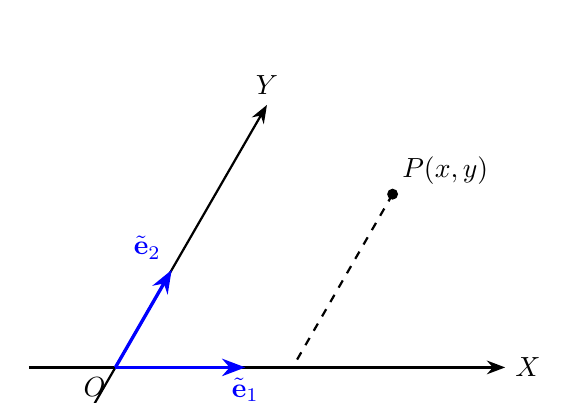
\begin{tikzpicture}[>=Stealth, scale=1.1]
  \draw[->, thick] (-1,0) -- (4.5,0) node[right] {$X$};
  \draw[->, thick] (240:0.6) -- (60:3.5) node[above] {$Y$};
  \node[below left] at (0,0) {$O$};
  \draw[->, very thick, blue] (0,0) -- (1.5,0) node[below] {$\tilde{\mathbf{e}}_1$};
  \draw[->, very thick, blue] (0,0) -- (60:1.3) node[above left] {$\tilde{\mathbf{e}}_2$};
  
  \coordinate (P) at (3.2, 2.0);
  \pgfmathsetmacro{\Py}{2.0}
  \pgfmathsetmacro{\Px}{3.2}
  \pgfmathsetmacro{\yv}{\Py / sin(60)}
  \pgfmathsetmacro{\xv}{\Px - \yv * cos(60)}
  \coordinate (P1) at (\xv, 0);
  \draw[dashed, thick] (P) -- (P1);
  \fill (P) circle (1.8pt) node[above right] {$P(x,y)$};
\end{tikzpicture}
\caption{$X$ 軸與點 $P(x,y)$}
\label{fig:4-3}
\end{figure}

\begin{definition}
一般地，給了一個方程式
\[ f(x, y) = 0 \]
設 $\Gamma_f = \{(x, y) \mid f(x, y) = 0\}$。我們說 $\Gamma_f$ 是方程式 $f(x, y) = 0$ 的軌跡，或說方程式 $f(x, y) = 0$ 描寫或代表 $\Gamma_f$，或說 $\Gamma_f$ 可以表成 $f(x, y) = 0$，也說 $f(x, y) = 0$ 與 $\Gamma_f$ 兩者是相應的，即 $\Gamma_f$ 是滿足 $f(x, y) = 0$ 之代數曲線。
\end{definition}

我們也注意到任何平行於 $X$ 軸的直線，可以表成
\[ y = c \]
而任何平行於 $Y$ 軸的直線則可表成
\[ x = c' \]
其中 $c$ 與 $c'$ 為實常數。

\begin{figure}[H]
\centering
\begin{subfigure}[b]{0.48\textwidth}
\centering
\begin{tikzpicture}[>=Stealth, scale=0.75]
  % General coordinates
  \draw[->, thick] (-2,0) -- (4,0) node[right] {$X$};
  \draw[->, thick] (240:1.5) -- (60:4.5) node[above] {$Y$};
  \node[below left] at (0,0) {$O$};
  
  \draw[->, very thick, blue] (0,0) -- (1,0) node[below] {$\tilde{\mathbf{e}}_1$};
  \draw[->, very thick, blue] (0,0) -- (60:2) node[above left] {$\tilde{\mathbf{e}}_2$};
  
  % y = c lines (parallel to X axis)
  % c = -1, 1/2, 3/2
  \pgfmathsetmacro{\sint}{sin(60)}
  \draw[thick] (-2, -1*\sint*2) -- (4, -1*\sint*2) node[right] {$y = -1$};
  \draw[thick] (-2, 0.5*\sint*2) -- (4, 0.5*\sint*2) node[right] {$y = \frac{1}{2}$};
  \draw[thick] (-2, 1.5*\sint*2) -- (4, 1.5*\sint*2) node[right] {$y = \frac{3}{2}$};
  
  % x = c' lines (parallel to Y axis)
  % c' = -1, 1.5, 2
  \draw[thick] ($(-1, -1.5) + (240:0.5)$) -- ($(-1, 3.5) + (60:0.5)$) node[above] {$x = -1$};
  \draw[thick] ($(1.5, -1.5) + (240:0.5)$) -- ($(1.5, 3.5) + (60:0.5)$) node[above] {$x = 1.5$};
  \draw[thick] ($(2, -1.5) + (240:0.5)$) -- ($(2, 3.5) + (60:0.5)$) node[above] {$x = 2$};
  
  \node[right, align=left] at (2.2, 2.5) {\footnotesize 其中 — 為單位長\\ \footnotesize $|\tilde{\mathbf{e}}_1| = 2$\\ \footnotesize $|\tilde{\mathbf{e}}_2| = 4$};
\end{tikzpicture}
\caption{一般座標系中的平行線族}
\label{fig:4-4-a}
\end{subfigure}
\hfill
\begin{subfigure}[b]{0.48\textwidth}
\centering
\begin{tikzpicture}[>=Stealth, scale=0.75]
  % Orthogonal coordinates
  \draw[->, thick] (-2.5,0) -- (4,0) node[right] {$X$};
  \draw[->, thick] (0,-2.5) -- (0,4) node[above] {$Y$};
  \node[below left] at (0,0) {$O$};
  
  \draw[->, very thick, blue] (0,0) -- (1,0) node[below] {$\mathbf{e}_1$};
  \draw[->, very thick, blue] (0,0) -- (0,1) node[left] {$\mathbf{e}_2$};
  
  % Horizontal lines
  \draw[thick] (-2.5, -1) -- (4, -1) node[right] {$y = -1$};
  \draw[thick] (-2.5, 0.5) -- (4, 0.5) node[right] {$y = \frac{1}{2}$};
  \draw[thick] (-2.5, 1.5) -- (4, 1.5) node[right] {$y = \frac{3}{2}$};
  
  % Vertical lines
  \draw[thick] (-1, -2.5) -- (-1, 4) node[above] {$x = -1$};
  \draw[thick] (1.5, -2.5) -- (1.5, 4) node[above] {$x = 1.5$};
  \draw[thick] (2, -2.5) -- (2, 4) node[above] {$x = 2$};
  
  \node[right, align=left] at (1.8, 2.5) {\footnotesize 其中 — 為單位長\\ \footnotesize $|\mathbf{e}_1| = |\mathbf{e}_2| = 1$};
\end{tikzpicture}
\caption{正交座標系中的平行線族}
\label{fig:4-4-b}
\end{subfigure}
\caption{平行於座標軸之直線族}
\label{fig:4-4}
\end{figure}

（圖 \ref{fig:4-4-a}）中諸橫線分別為當 $c = -2/2, 0, 1/2, 3/2$ 時，
\[ y = c \]
之軌跡，諸縱線則分別為當 $c' = -1, 0, 1.5, 2$ 時，
\[ x = c' \]
之軌跡，其中 $|\tilde{\mathbf{e}}_1| = 1, |\tilde{\mathbf{e}}_2| = 2$\footnote{\phantomsection\label{note:b3-ch4-p136-fig4-4-a-scale}【校訂註】原書圖 4-4-a 註記印作「$|\tilde{\mathbf{e}}_1| = 2, |\tilde{\mathbf{e}}_2| = 4$」，下文行文說明作「$|\tilde{\mathbf{e}}_1| = 1, |\tilde{\mathbf{e}}_2| = 2$」，兩者相差二倍刻度比例。正文忠實保留原文對比。}。圖 \ref{fig:4-4-b} 則為取正交座標時之特殊情形。

稍進一步我們要考慮較一般的方程式
\begin{equation}
-2x + y = 3
\label{eq:b3-4-1}
\end{equation}
我們用描點法在座標圖上點出這方程式的軌跡。方法是這樣：\eqref{eq:b3-4-1} 式中既然有 $x$，則把一些值，比如 $-5, -1, 0, 1.5, 4, \dots$ 等值代入 \eqref{eq:b3-4-1}，求得相應之 $y$，按序為 $-7, 1, 3, 6, 11$。亦即：$(-5, -7), (-1, 1), (0, 3), (1.5, 6), (4, 11), \dots$ 等點皆在方程式 \eqref{eq:b3-4-1} 的軌跡上，把這些點在座標圖上描出來，約略可以猜想這軌跡也許是一條直線（如圖 \ref{fig:4-5}）。

\begin{figure}[H]
\centering
\begin{subfigure}[b]{0.48\textwidth}
\centering
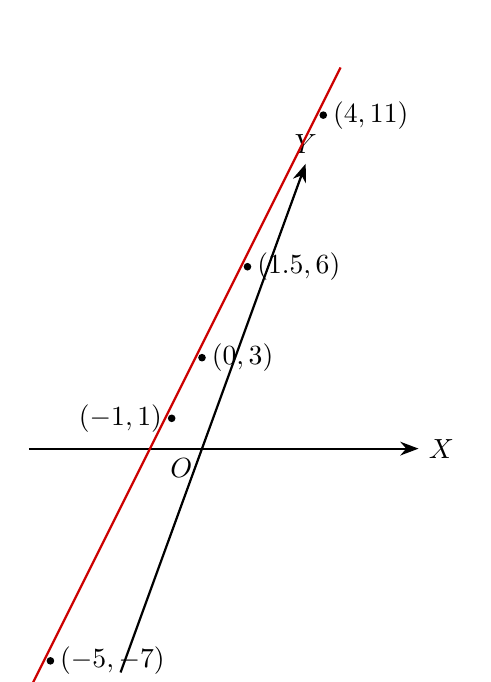
\begin{tikzpicture}[>=Stealth, scale=0.55]
  % General coordinates
  \draw[->, thick] (-4,0) -- (5,0) node[right] {$X$};
  \draw[->, thick] (250:5.5) -- (70:7) node[above] {$Y$};
  \node[below left] at (0,0) {$O$};
  
  \coordinate (P1) at (-3.5, -4.9);
  \coordinate (P2) at (-0.7, 0.7);
  \coordinate (P3) at (0, 2.1);
  \coordinate (P4) at (1.05, 4.2);
  \coordinate (P5) at (2.8, 7.7);
  
  \draw[thick, red!80!black] (-4, -5.6) -- (3.2, 8.8);
  \fill (P1) circle (2.5pt) node[right] {$(-5, -7)$};
  \fill (P2) circle (2.5pt) node[left] {$(-1, 1)$};
  \fill (P3) circle (2.5pt) node[right] {$(0, 3)$};
  \fill (P4) circle (2.5pt) node[right] {$(1.5, 6)$};
  \fill (P5) circle (2.5pt) node[right] {$(4, 11)$};
\end{tikzpicture}
\caption{一般座標系中直線描點}
\label{fig:4-5-a}
\end{subfigure}
\hfill
\begin{subfigure}[b]{0.48\textwidth}
\centering
\begin{tikzpicture}[>=Stealth, scale=0.55]
  % Orthogonal coordinates
  \draw[->, thick] (-4,0) -- (5,0) node[right] {$X$};
  \draw[->, thick] (0,-5.5) -- (0,7.5) node[above] {$Y$};
  \node[below left] at (0,0) {$O$};
  
  % -2x + y = 3 => y = 2x + 3
  % Points scaled by 0.6
  \coordinate (P1) at (-5*0.6, -7*0.6);
  \coordinate (P2) at (-1*0.6, 1*0.6);
  \coordinate (P3) at (0, 3*0.6);
  \coordinate (P4) at (1.5*0.6, 6*0.6);
  \coordinate (P5) at (4*0.6, 11*0.6);
  
  \draw[thick, red!80!black] (-3.5*0.6, -4*0.6) -- (2.5*0.6, 8*0.6);
  \fill (P1) circle (2.5pt) node[right] {$(-5, -7)$};
  \fill (P2) circle (2.5pt) node[left] {$(-1, 1)$};
  \fill (P3) circle (2.5pt) node[right] {$(0, 3)$};
  \fill (P4) circle (2.5pt) node[right] {$(1.5, 6)$};
  \fill (P5) circle (2.5pt) node[right] {$(4, 11)$};
\end{tikzpicture}
\caption{正交座標系中直線描點}
\label{fig:4-5-b}
\end{subfigure}
\caption{方程式 $-2x+y=3$ 之描點軌跡}
\label{fig:4-5}
\end{figure}

\subsubsection*{作業 3}
試在正交座標圖上描出下列諸式的軌跡
\begin{enumerate}[label=(\roman*), leftmargin=2em]
  \item $x + y = 3$
  \item $5x - 6y + 2 = 0$
  \item $2x - y = 2$
\end{enumerate}

要是 \eqref{eq:b3-4-1} 式中給予不同的係數，我們不斷描圖，每次都會發覺它所代表的是一直線。我們將在本節節尾敘述，並於 § 4-3 證明
\begin{equation}
ax + by + c = 0
\label{eq:b3-4-2}
\end{equation}
「是直線的一般方程式表示」。

現在，我們注意到 \eqref{eq:b3-4-2} 式若不是 $x$ 與 $y$ 的一次方程便可能會有其他種軌跡出現，也有可能軌跡本身根本就是一個空集合。

\begin{example}[論例 1]
在這裏，我們採用正交座標系。
\begin{enumerate}[label=(\roman*), leftmargin=2em]
  \item $f(x, y) = x^2 + y^2 = 1$ 代表一個以 1 為半徑的圓，道理是根據畢氏定理，$x^2 + y^2$ 其實是 $P(x, y)$ 到原點 $O(0, 0)$ 的距離的平方。當這距離的平方固定為 1 時，距離便固定了，這樣 $P(x, y)$ 描出一個以 $O(0, 0)$ 為心，半徑為 1 的圓（見圖 \ref{fig:4-6}）。
  \item $f(x, y) = x^2 + y^2 = 0$ 的軌跡，只含有原點 $O(0, 0)$ 一個點。
  \item $f(x, y) = x^2 + y^2 = -1$ 的軌跡是一個空集合，因為找不到兩個實數 $x$ 與 $y$ 其平方和為負數。
\end{enumerate}
\end{example}

\begin{figure}[H]
\centering
\begin{subfigure}[b]{0.45\textwidth}
\centering
\begin{tikzpicture}[>=Stealth, scale=1.3]
  \draw[->, thick] (-1.5,0) -- (1.8,0) node[right] {$X$};
  \draw[->, thick] (0,-1.5) -- (0,1.8) node[above] {$Y$};
  \node[below left] at (0,0) {$O$};
  \draw[thick] (0,0) circle (1);
  \coordinate (P) at (60:1);
  \draw[thick] (0,0) -- (P) node[midway, above left] {$1$};
  \draw[dashed, thick] (P) -- (P |- 0,0) node[midway, right] {$y$};
  \draw[thick] (0,0) -- (P |- 0,0) node[midway, below] {$x$};
  \fill (P) circle (1.5pt) node[above right] {$P(x,y)$};
  \node[right] at (0.4, 0.5) {\footnotesize 其中 — 為單位長};
\end{tikzpicture}
\caption{單位圓 $x^2+y^2=1$}
\label{fig:4-6}
\end{subfigure}
\hfill
\begin{subfigure}[b]{0.48\textwidth}
\centering
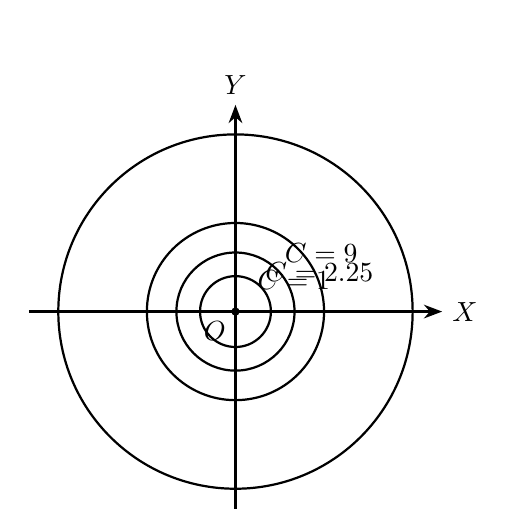
\begin{tikzpicture}[>=Stealth, scale=0.75]
  \draw[->, thick] (-3.5,0) -- (3.5,0) node[right] {$X$};
  \draw[->, thick] (0,-3.5) -- (0,3.5) node[above] {$Y$};
  \node[below left] at (0,0) {$O$};
  \draw[thick] (0,0) circle (0.6);
  \draw[thick] (0,0) circle (1.0) node[above right=6pt] {$C=1$};
  \draw[thick] (0,0) circle (1.5) node[above right=10pt] {$C=2.25$};
  \draw[thick] (0,0) circle (3.0) node[above right=20pt] {$C=9$};
  \fill (0,0) circle (2pt);
\end{tikzpicture}
\caption{同心圓族 $x^2+y^2=C$}
\label{fig:4-7}
\end{subfigure}
\caption{二次方程軌跡}
\end{figure}

（其實上面三個例子，可看成 $C$ 也在變動的一個方程式
\begin{equation}
x^2 + y^2 = C
\label{eq:b3-4-3}
\end{equation}
所表示的線族。當 $C$ 從正值變小，變 0，再變成負值的過程中，我們得到各個不同的圓的軌跡，它的半徑逐漸縮小；縮到一個點後，就躍變為空集合）（見圖 \ref{fig:4-7}）。

\subsubsection*{丙、直線的一般方程式表示}

對於一般座標系，我們有

\begin{theorem}
\label{thm:b3-4-1}
\begin{enumerate}[label=(\Roman*), leftmargin=2em]
  \item 取定一個一般的座標系 $(O; \tilde{\mathbf{e}}_1, \tilde{\mathbf{e}}_2)$，一次方程式
  （假定 $a$ 與 $b$ 不全為 0）
  \begin{equation}
  ax + by + c = 0
  \label{eq:b3-4-4}
  \end{equation}
  的軌跡一定是直線。
  \item 反過來，給了一條直線，必存在適當的實數 $a, b, c$，使得 \eqref{eq:b3-4-4} 式的軌跡正好是這條給定的直線。
  \item 兩個一次方程式：
  \[ a_1 x + b_1 y + c_1 = 0 \quad\text{及}\quad a_2 x + b_2 y + c_2 = 0 \]
  代表同一直線的充要條件則是存在一實數 $k \neq 0$ 使得
  \[ a_1 = k a_2, \quad b_1 = k b_2, \quad c_1 = k c_2. \]
  即：所有對應係數成比例。
\end{enumerate}
\end{theorem}

我們不急著要證明這個定理，要把它們放到 § 4-3 才講。

本節乙段反覆指示給我們一個對照：代數中一個方程式 $f(x, y) = 0$ 相當於幾何中該方程的軌跡 $\Gamma_f$。本段之定理 \ref{thm:b3-4-1}，更告訴我們：代數上的二元一次方程式恰好相當於平面上的直線，在以後諸節裏，我們要看到這些直線的幾何性質，如傾斜度、平行與垂直、共點等觀念怎樣轉化為所對應的二元一次方程式的表現上來。

一般時候，若有兩個方程式
\[ f(x, y) = 0 \quad\text{與}\quad g(x, y) = 0 \]
設 $\Gamma_f, \Gamma_g$ 分別是它們軌跡，即
\[ \Gamma_f = \{(x, y) \mid f(x, y) = 0\}, \quad \Gamma_g = \{(x, y) \mid g(x, y) = 0\} \]
則交集 $\Gamma_f \cap \Gamma_g$ 成為同時滿足 $f(x, y) = 0$ 與 $g(x, y) = 0$ 的點 $(x, y)$ 之集合，亦即：交集 $\Gamma_f \cap \Gamma_g$ 中的點 $(x, y)$ 正好是聯立方程式
\[ \begin{cases} f(x, y) = 0 \\ g(x, y) = 0 \end{cases} \]
的解。這解嚴格說是一個集合（必要時稱它為解集合）它可能代表一個點，可能兩個點，也可能是空集合，或無限多點。

\begin{example}[例 3]
\begin{enumerate}[label=(\roman*), leftmargin=2em]
  \item 聯立方程式 $\begin{cases} x = c' \\ y = c \end{cases}$ 的解相當於兩直線 $x = c'$ 與 $y = c$ 的交點 $(c', c)$。
  \item 直線 $x - y = 1$ 與 $x + y = 3$ 之交點的求法為：
  解聯立方程式 $\begin{cases} x - y = 1 \\ x + y = 3 \end{cases}$，得 $\begin{cases} x = 2 \\ y = 1 \end{cases}$，即交點為 $(2, 1)$。
  \item 設所取座標系為正交座標系，則直線 $L_1 : x + 2y = 3$ 與圓 $C : x^2 + y^2 = 1$ 無交點。
  因求解聯立方程式 $\begin{cases} x + 2y = 3 \\ x^2 + y^2 = 1 \end{cases}$ 時，先得 $x = 3 - 2y$，代入 $x^2 + y^2 = 1$ 中得：$9 - 12y + 4y^2 + y^2 = 1$，即 $5y^2 - 12y + 8 = 0$。其判別式 $144 - 160 = -16 < 0$，故無解〔指無實數解〕。
  \item 設所取座標系為正交座標系，要求直線 $L_2 : x + 2y = 1$ 與圓 $C : x^2 + y^2 = 1$ 的交點，即欲解聯立方程式：
  \[ \begin{cases} x + 2y = 1 \\ x^2 + y^2 = 1 \end{cases} \]
  此時從第一式以 $x = 1 - 2y$ 代入第二式，得 $(1 - 2y)^2 + y^2 = 1$，$y = 0$ 或 $\frac{4}{5}$；$x = 1$ 或 $-\frac{3}{5}$。故 $(1, 0)$ 與 $(-\frac{3}{5}, \frac{4}{5})$ 為所求的兩個交點。
  \item $2x + y = 1$ 與 $4x + 2y - 2 = 0$ 兩方程式軌跡之交集仍為直線 $2x + y = 1$，故為無限多解。
\end{enumerate}
\end{example}

\begin{figure}[H]
\centering
\begin{subfigure}[b]{0.45\textwidth}
\centering
\begin{tikzpicture}[>=Stealth, scale=0.8]
  \draw[->, thick] (-1.5,0) -- (3.5,0) node[right] {$X$};
  \draw[->, thick] (240:1) -- (60:3.5) node[above] {$Y$};
  \node[below left] at (0,0) {$O$};
  \draw[->, very thick, blue] (0,0) -- (1,0) node[below] {$\tilde{\mathbf{e}}_1$};
  \draw[->, very thick, blue] (0,0) -- (60:1) node[above left] {$\tilde{\mathbf{e}}_2$};
  
  \coordinate (P) at (2, 1.8);
  \draw[thick] (-1, 1.8) -- (3.5, 1.8) node[right] {$y = c$};
  \draw[thick] ($(2, -1) + (240:0.3)$) -- ($(2, 2.5) + (60:0.3)$) node[above] {$x = c'$};
  \fill (2.6, 1.8) circle (2pt) node[below right] {$(c', c)$};
\end{tikzpicture}
\caption{兩直線交點}
\label{fig:4-8}
\end{subfigure}
\hfill
\begin{subfigure}[b]{0.45\textwidth}
\centering
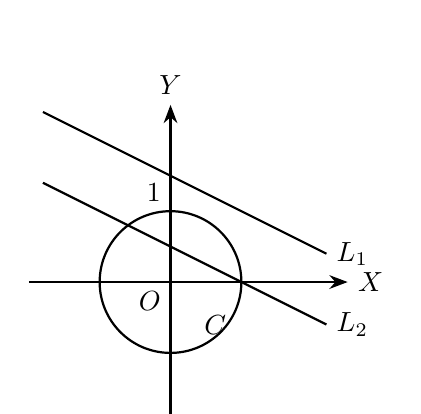
\begin{tikzpicture}[>=Stealth, scale=0.9]
  \draw[->, thick] (-2,0) -- (2.5,0) node[right] {$X$};
  \draw[->, thick] (0,-2) -- (0,2.5) node[above] {$Y$};
  \node[below left] at (0,0) {$O$};
  \draw[thick] (0,0) circle (1) node[below right=12pt] {$C$};
  \node[above left] at (0,1) {$1$};
  
  % L1: x + 2y = 3 -> y = -0.5x + 1.5
  \draw[thick] (-1.8, 2.4) -- (2.2, 0.4) node[right] {$L_1$};
  % L2: x + 2y = 1 -> y = -0.5x + 0.5
  \draw[thick] (-1.8, 1.4) -- (2.2, -0.6) node[right] {$L_2$};
\end{tikzpicture}
\caption{直線與圓的相交情形}
\label{fig:4-9}
\end{subfigure}
\caption{聯立方程式之幾何軌跡}
\end{figure}

\begin{example}[例 4]
設根據一正交座標系有 $A(0, 0), B(2, 1)$ 兩點，而 $P$ 為一動點，使得 $\overline{PA} = \overline{PB}$。試求 $P$ 點的軌跡所相應的方程式。
\end{example}

\begin{proof}[解]
因 $\overline{PA} = \sqrt{x^2+y^2}, \overline{PB} = \sqrt{(x-2)^2+(y-1)^2}$，其中 $P$ 之座標為 $P(x, y)$。故有
\[ \overline{PA} = \overline{PB} \iff \overline{PA}^2 = \overline{PB}^2 \]
即
\[ x^2 + y^2 = (x-2)^2 + (y-1)^2 \]
整理得 $4x + 2y = 5$，此即為 $P$ 點軌跡所相應的方程式。

故由定理 \ref{thm:b3-4-1} 知，$P$ 的軌跡為一直線，即線段 $AB$ 的垂直平分線。
\end{proof}

\subsubsection*{作業 4}
試求 $P$ 點的軌跡，並描點圖示之。
\begin{enumerate}[label=\roman*), leftmargin=2em]
  \item 同上例之 $A, B$ 點，使 $\overline{PA} = 2\overline{PB}$。
  \item 設 $A(-1, 0), B(1, 0)$ 使 $\overline{PA} + \overline{PB} = 3$。
  \item $P$ 與 $(2, 0)$ 之距離恒等於其與 $y$ 軸之距離。
\end{enumerate}
試問在各小題中，$P$ 點的軌跡是一直線嗎？

\subsubsection*{習題 4-1}

\begin{enumerate}[label=\arabic*., leftmargin=2em]
  \item 設相關於正交座標系 $(O; \mathbf{e}_1, \mathbf{e}_2)$，兩向量 $\tilde{\mathbf{e}}_1, \tilde{\mathbf{e}}_2$ 之座標為
  \[ \tilde{\mathbf{e}}_1 = (0, 2), \quad \tilde{\mathbf{e}}_2 = (1, 2) \]
  問 $(O; \tilde{\mathbf{e}}_1, \tilde{\mathbf{e}}_2)$ 是否構成一座標系？試繪圖表示根據座標系 $(O; \tilde{\mathbf{e}}_1, \tilde{\mathbf{e}}_2)$ 作成的座標為 $(1, 1), (2, 2), (2, 3)$ 之點。
  
  \item 設相關於正交座標系 $(O; \mathbf{e}_1, \mathbf{e}_2)$，兩向量 $\tilde{\mathbf{e}}_1, \tilde{\mathbf{e}}_2$ 之座標為
  \[ \tilde{\mathbf{e}}_1 = (1, 1), \quad \tilde{\mathbf{e}}_2 = (-1, 1) \]
  試繪圖表示根據 $(O; \tilde{\mathbf{e}}_1, \tilde{\mathbf{e}}_2)$ 做成的座標為 $(3, 1), (-1, 1), (1, 2)$ 之點。並問這些點相關於原座標系 $(O; \mathbf{e}_1, \mathbf{e}_2)$ 之座標為何？
  
  \item 分別用題 1 與題 2 中的座標系 $(O; \tilde{\mathbf{e}}_1, \tilde{\mathbf{e}}_2)$，繪圖表出下式軌跡
  \begin{enumerate}[label=\roman*), leftmargin=2em]
    \item $x + y = 1$
    \item $x = -3$
    \item $x - 3y + 5 = 0$
    \item $y = 2$
  \end{enumerate}
  
  \item 對正交座標系，試求一直線方程式，使其平行於 $Y$ 軸，且在點 $(2, 5)$ 左邊 6 單位距離。
  
  \item 試求與點 $(0, 0)$ 距離恒為 10 的軌跡方程式。
  
  \item 曲線 $y^2 = 4x$ 與直線 $2x + 8y + 2 = 0$ 是否相交？
  
  \item 在下面兩圖中，分別約略估計向量 $\mathbf{a}$ 相關於所給座標系 $(O; \tilde{\mathbf{e}}_1, \tilde{\mathbf{e}}_2)$ 的座標（即：向量座標成分）
  
  \begin{center}
  \begin{tikzpicture}[>=Stealth, scale=0.9]
    % (1)
    \begin{scope}[shift={(0,0)}]
      \node at (0, 2.5) {(1)};
      \coordinate (O) at (0,0);
      \coordinate (E1) at (1.8,-0.2);
      \coordinate (E2) at (0.3,-1.5);
      \coordinate (A) at (-0.8, 1.8);
      \draw[->, very thick] (O) -- (E1) node[above right] {$\tilde{\mathbf{e}}_1$};
      \draw[->, very thick] (O) -- (E2) node[below right] {$\tilde{\mathbf{e}}_2$};
      \draw[->, very thick, red!80!black] (O) -- (A) node[above left] {$\mathbf{a}$};
      \node[below left] at (O) {$O$};
    \end{scope}
    
    % (2)
    \begin{scope}[shift={(5,0)}]
      \node at (0, 2.5) {(2)};
      \coordinate (O) at (0,0);
      \coordinate (E1) at (2.0, 0.8);
      \coordinate (E2) at (-0.8, 0.5);
      \coordinate (A) at (0.4, -1.8);
      \draw[->, very thick] (O) -- (E1) node[above right] {$\tilde{\mathbf{e}}_1$};
      \draw[->, very thick] (O) -- (E2) node[above left] {$\tilde{\mathbf{e}}_2$};
      \draw[->, very thick, red!80!black] (O) -- (A) node[below right] {$\mathbf{a}$};
      \node[below left] at (O) {$O$};
    \end{scope}
  \end{tikzpicture}
  \end{center}
  
  例如 在左圖中約有
  \[ \mathbf{a} = 0.4\tilde{\mathbf{e}}_1 + 1.8\tilde{\mathbf{e}}_2 \]
  故 $\mathbf{a}$ 相關於 $(O; \tilde{\mathbf{e}}_1, \tilde{\mathbf{e}}_2)$ 之座標為 $(0.4, 1.8)$。
  
  \begin{center}
  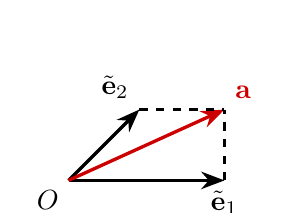
\begin{tikzpicture}[>=Stealth, scale=0.9]
    \coordinate (O) at (0,0);
    \coordinate (E1) at (2.2, 0);
    \coordinate (E2) at (1.0, 1.0);
    \coordinate (A) at (2.2, 1.0);
    \draw[->, very thick] (O) -- (E1) node[below] {$\tilde{\mathbf{e}}_1$};
    \draw[->, very thick] (O) -- (E2) node[above left] {$\tilde{\mathbf{e}}_2$};
    \draw[->, very thick, red!80!black] (O) -- (A) node[above right] {$\mathbf{a}$};
    \draw[dashed, thick] (E1) -- (A);
    \draw[dashed, thick] (E2) -- (A);
    \node[below left] at (O) {$O$};
  \end{tikzpicture}
  \end{center}
\end{enumerate}

\subsection{直線的參數式及座標兩點式}
\label{sec:4-2}

本節取定一個一般座標系 $(O; \tilde{\mathbf{e}}_1, \tilde{\mathbf{e}}_2)$，所出現的點或向量的座標都是根據這一座標系。

平面上相異兩點 $A(x_1, y_1), B(x_2, y_2)$ 可決定出一條直線 $L$，$L$ 稱為過 $A, B$ 的直線。我們來看看 $L$ 的代數表示：

\subsubsection*{甲、參數式}

\paragraph*{(I) 直線的向量參數表示：}
設 $\mathbf{a} = \vec{OA}, \mathbf{b} = \vec{OB}$，則平面上一點 $P(x, y)$ 會落在 $A, B$ 所決定的直線 $L$ 上的充分必要條件是 $\vec{AP}$ 所代表的向量為 $\vec{AB}$ 所代表的相應的實倍數。亦即
\[ \vec{AP} = t\vec{AB}; \quad t \in \mathbb{R} \]
今取 $\mathbf{c} = \vec{OP}$，則上述條件因
\begin{align*}
\mathbf{c} &= \vec{OP} = \vec{OA} + \vec{AP} \\
&= \vec{OA} + t(\vec{OB} - \vec{OA}) \\
&= \mathbf{a} + t(\mathbf{b} - \mathbf{a})
\end{align*}
而化成
\begin{equation}
\mathbf{c} = (1 - t)\mathbf{a} + t\mathbf{b}
\label{eq:b3-4-5}
\end{equation}
其中 $t$ 稱為式中之參數。
或 $\mathbf{c} = \alpha\mathbf{a} + \beta\mathbf{b}$，其中 $\alpha, \beta$ 為滿足 $\alpha + \beta = 1$ 之兩實數。這便是直線的向量參數表示式。

\begin{figure}[H]
\centering
\begin{tikzpicture}[>=Stealth, scale=1.1]
  \coordinate (O) at (0,0);
  \coordinate (A) at (3,0.5);
  \coordinate (B) at (1,2.0);
  
  % Line L through A and B
  \coordinate (Lstart) at ($(A)!-0.6!(B)$);
  \coordinate (Lend) at ($(A)!1.6!(B)$);
  \draw[thick] (Lstart) -- (Lend) node[below right] {$L$};
  
  \draw[->, thick] (O) -- (A) node[midway, below] {$\mathbf{a}$};
  \draw[->, thick] (O) -- (B) node[midway, left] {$\mathbf{b}$};
  
  \coordinate (P) at ($(A)!0.5!(B)$);
  \draw[->, thick] (O) -- (P) node[above left] {$\mathbf{c}$};
  \draw[->, very thick, red!80!black] (A) -- (P) node[midway, below left] {$t(\mathbf{b}-\mathbf{a})$};
  
  \fill (O) circle (1.8pt) node[below left] {$O$};
  \fill (A) circle (1.8pt) node[right] {$A$};
  \fill (B) circle (1.8pt) node[above left] {$B$};
  \fill (P) circle (1.8pt) node[above right] {$P$};
  
  % Region markers
  \node[above right, rotate=-37] at ($(A)!-0.3!(B)$) {$t < 0$};
  \node[above right, rotate=-37] at ($(A)!0.5!(B) + (0, 0.4)$) {$1 \ge t \ge 0$};
  \node[above right, rotate=-37] at ($(A)!1.3!(B)$) {$t > 1$};
\end{tikzpicture}
\caption{直線的向量參數表示}
\label{fig:4-10}
\end{figure}

注意 當 $t = 0$ 時，$\mathbf{c} = \mathbf{a}$，而當 $t = 1$ 時，$\mathbf{c} = \mathbf{b}$。

現在分別考慮 \eqref{eq:b3-4-5} 式兩端的座標成分，可得

\paragraph*{(II) 直線之座標參數表示：}
過相異兩點 $A(x_1, y_1)$ 與 $B(x_2, y_2)$ 的直線 $L$ 上的點 $P(x, y)$，恰好是那些座標可以表示成下列 \eqref{eq:b3-4-6} 式的點
\begin{equation}
\begin{cases}
x = x_1 + t(x_2 - x_1) \\
y = y_1 + t(y_2 - y_1)
\end{cases}
\label{eq:b3-4-6}
\end{equation}
或
\begin{equation}
\begin{cases}
x = (1 - t)x_1 + tx_2 \\
y = (1 - t)y_1 + ty_2
\end{cases}
\label{eq:b3-4-7}
\end{equation}

\begin{example}[例 5]
設通過 $A(0, 2), B(2, 1)$ 的直線為 $L$，對 $L$ 上任一點 $P(x, y)$，
\[ x = (1 - t)\cdot 0 + t\cdot 2 = 2t, \quad y = (1 - t)\cdot 2 + t\cdot 1 = 2 - t. \]
\end{example}

\begin{figure}[H]
\centering
\begin{tikzpicture}[>=Stealth, scale=1.1]
  \draw[->, thick] (-1,0) -- (4,0) node[right] {$X$};
  \draw[->, thick] (250:0.8) -- (70:3.5) node[above] {$Y$};
  \node[below left] at (0,0) {$O$};
  
  \draw[->, very thick, blue] (0,0) -- (1,0) node[below] {$\tilde{\mathbf{e}}_1$};
  \draw[->, very thick, blue] (0,0) -- (70:1) node[above left] {$\tilde{\mathbf{e}}_2$};
  
  % Points A(0, 2) in basis => 2 * e2_dir
  \coordinate (A) at ($(0,0) + (70:2.0)$);
  % B(2, 1) in basis => 2 * (1, 0) + 1 * (70:1)
  \coordinate (B) at ($(2,0) + (70:1.0)$);
  
  \draw[thick, red!80!black] ($(A)!-0.4!(B)$) -- ($(A)!1.5!(B)$);
  \coordinate (P) at ($(A)!0.6!(B)$);
  
  \draw[->, thick] (0,0) -- (A);
  \draw[->, thick] (0,0) -- (B);
  \draw[->, thick] (0,0) -- (P);
  
  \fill (A) circle (1.8pt) node[above right] {$A(0,2)$};
  \fill (B) circle (1.8pt) node[right] {$B(2,1)$};
  \fill (P) circle (1.8pt) node[above right] {$P(2t, 2-t)$};
\end{tikzpicture}
\caption{直線參數表示實例}
\label{fig:4-11}
\end{figure}

即 $L$ 的座標參數式為
\[ \begin{cases} x = 2t \\ y = 2 - t \end{cases} \]
亦即 $P$ 點座標為 $(2t, 2 - t)$。

用向量來表示也是一樣：
\[ \mathbf{a} = \vec{OA} = (0, 2), \quad \mathbf{b} = \vec{OB} = (2, 1) \]
則 $\mathbf{c} = \vec{OP} = (1 - t)\mathbf{a} + t\mathbf{b} = (2t, 2 - t)$。

\subsubsection*{作業 5}
設 $\mathbf{a} = \vec{OA}, \mathbf{b} = \vec{OB}$ 其座標如下，求過 $A, B$ 兩點之直線 $L$ 之參數式：
\begin{enumerate}[label=(\roman*), leftmargin=2em]
  \item $\mathbf{a} = (6, 2), \mathbf{b} = (3, 1)$
  \item $\mathbf{a} = (5, 3), \mathbf{b} = (3, 5)$
  \item $\mathbf{a} = (3, -1), \mathbf{b} = (2, -6)$
  \item $\mathbf{a} = (2, 1), \mathbf{b} = (0, 9)$
\end{enumerate}

\begin{example}[例 6]
同例 5 當 $t = \frac{1}{2}$ 時，$\vec{OP} = (1, \frac{3}{2})$，此時 $P$ 為 $AB$ 之中點，$P = P(1, \frac{3}{2})$。
\end{example}

\begin{example}[例 7]
同前，若 $P$ 點內分 $\overline{AB}$ 成 $1 : 2$，即 $\overline{AP} : \overline{PB} = 1 : 2$，則 $P$ 之座標如何？
\end{example}

\begin{proof}[解]
因 $\vec{AP} = \frac{1}{3}\vec{AB}$，故有 $t = \frac{1}{3}$，則 $\vec{OP} = (\frac{2}{3}, \frac{5}{3})$ 或 $P = P(\frac{2}{3}, \frac{5}{3})$。
\end{proof}

\begin{example}[論例 2]
一般來說給了兩點 $A(x_1, y_1), B(x_2, y_2)$，而 $P$ 點內分 $\overline{AB}$ 為 $a : b$，則 $P$ 之座標如何？
\end{example}

\begin{proof}[解]
因 $\vec{AP} = \frac{a}{a+b}\vec{AB}$，故有 $t = \frac{a}{a+b}$，則 $P$ 點之座標為
\[ \left( \frac{b x_1 + a x_2}{a + b}, \frac{b y_1 + a y_2}{a + b} \right). \qedhere \]
\end{proof}

\subsubsection*{作業 6}
\begin{enumerate}[label=(\roman*), leftmargin=2em]
  \item 設 $A = (-3, 5), B = (2, 1)$，試求通過 $A, B$ 兩點的直線的參數表示。
  \item 若 $P$ 點內分 $\overline{AB}$ 成 $1 : 3$（即 $\overline{AP} : \overline{PB} = 1 : 3$），試求 $P$ 點的座標。
  \item 若 $Q$ 點外分 $\overline{AB}$ 成 $1 : 3$（即 $\overline{AQ} : \overline{QB} = 1 : 3$），則 $Q$ 點的座標如何？
\end{enumerate}

\subsubsection*{乙、直線的各種代數表示式}

\paragraph*{(I) 直線的兩點式}
將 \eqref{eq:b3-4-6} 式整理得
\[ x - x_1 = t(x_2 - x_1) \quad\text{或}\quad t(y_2 - y_1) = y - y_1 \]
兩式相乘，兩端消去 $t$，得
\begin{equation}
(x - x_1)(y_2 - y_1) - (y - y_1)(x_2 - x_1) = 0
\label{eq:b3-4-8}
\end{equation}
〔注意 消去 $t$ 時，要求 $t \neq 0$。但 $t = 0$ 表示 $P$ 與 $A$ 點重合，即 $x = x_1, y = y_1$，故 \eqref{eq:b3-4-8} 式仍然成立。〕

另一方面，滿足 \eqref{eq:b3-4-8} 式的點亦必在直線 $L$ 上，道理是：
\begin{enumerate}[label=(\alph*), leftmargin=2em]
  \item 假如 $x_2 - x_1$ 與 $y_2 - y_1$ 皆不為 0，則 \eqref{eq:b3-4-8} 式可以化成
  \[ \frac{x - x_1}{x_2 - x_1} = \frac{y - y_1}{y_2 - y_1} \]
  設這個比例為 $t$，則有
  \[ \begin{cases} x = x_1 + t(x_2 - x_1) \\ y = y_1 + t(y_2 - y_1) \end{cases} \]
  由 \eqref{eq:b3-4-6} 式可知，滿足 \eqref{eq:b3-4-8} 式的點 $P(x, y)$ 必在 $L$ 上。
  
  \item 假如 $x_2 - x_1$ 及 $y_2 - y_1$ 中有一為 0，不妨假定是
  \[ y_2 - y_1 = 0 \]
  則 $x_2 - x_1 \neq 0$〔因 $A(x_1, y_1)$ 與 $B(x_2, y_2)$ 兩點相異，不能 $y_1 = y_2$，又 $x_1 = x_2$。〕
  
  這時，點 $A$ 與點 $B$ 的座標有相同的 $y$ 成分，其決定出來的直線 $L$ 應平行於 $X$ 軸，表為方程式，則
  \[ L : y = y_1 \]
  但 \eqref{eq:b3-4-8} 式也正是這樣的式子，因 $y_2 - y_1 = 0$，使 \eqref{eq:b3-4-8} 式變成
  \[ -(y - y_1)(x_2 - x_1) = 0 \]
  而 $x_2 - x_1 \neq 0$，又引出 $y - y_1 = 0$ 即 $y = y_1$。亦即滿足 \eqref{eq:b3-4-8} 式的點，皆在 $L$ 上。
\end{enumerate}

總結一下，\eqref{eq:b3-4-8} 式的軌跡恰好就是由相異兩點 $A(x_1, y_1)$ 與 $B(x_2, y_2)$ 決定出來的直線 $L$，這方程式就稱為直線的兩點式。

\begin{figure}[H]
\centering
\begin{subfigure}[b]{0.48\textwidth}
\centering
\begin{tikzpicture}[>=Stealth, scale=0.8]
  \draw[->, thick] (-1,0) -- (4.5,0) node[right] {};
  \draw[->, thick] (250:1.5) -- (70:3.5) node[above] {};
  \node[below left] at (0,0) {$O$};
  \draw[->, very thick, blue] (0,0) -- (1.5,0) node[below] {$\tilde{\mathbf{e}}_1$};
  \draw[->, very thick, blue] (0,0) -- (70:1) node[above left] {$\tilde{\mathbf{e}}_2$};
  
  \coordinate (A) at (3.5, 0.4);
  \coordinate (B) at (1.8, 1.8);
  \draw[thick, red!80!black] ($(A)!-0.4!(B)$) -- ($(A)!1.5!(B)$);
  \fill (A) circle (2pt) node[right] {$A(x_1, y_1)$};
  \fill (B) circle (2pt) node[above right] {$B(x_2, y_2)$};
\end{tikzpicture}
\caption{一般座標系兩點直線}
\label{fig:4-12-a}
\end{subfigure}
\hfill
\begin{subfigure}[b]{0.48\textwidth}
\centering
\begin{tikzpicture}[>=Stealth, scale=0.8]
  \draw[->, thick] (-1,0) -- (4.5,0) node[right] {$X$};
  \draw[->, thick] (0,-1) -- (0,3.5) node[above] {$Y$};
  \node[below left] at (0,0) {$O$};
  \draw[->, very thick, blue] (0,0) -- (1,0) node[below] {$\mathbf{e}_1$};
  \draw[->, very thick, blue] (0,0) -- (0,1) node[left] {$\mathbf{e}_2$};
  
  \coordinate (A) at (2.0, 0);
  \coordinate (B) at (0.5, 2.0);
  \draw[thick, red!80!black] ($(A)!-0.4!(B)$) -- ($(A)!1.4!(B)$);
  \fill (A) circle (2pt) node[below right] {$A(x_1, y_1)$};
  \fill (B) circle (2pt) node[above right] {$B(x_2, y_2)$};
\end{tikzpicture}
\caption{正交座標系兩點直線}
\label{fig:4-12-b}
\end{subfigure}
\caption{直線兩點式}
\label{fig:4-12}
\end{figure}

\begin{figure}[H]
\centering
\begin{subfigure}[b]{0.48\textwidth}
\centering
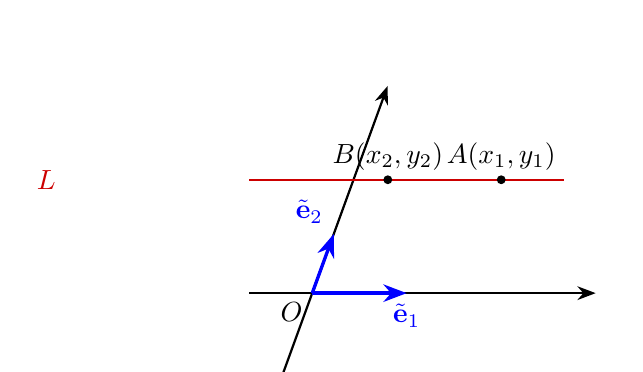
\begin{tikzpicture}[>=Stealth, scale=0.8]
  \draw[->, thick] (-1,0) -- (4.5,0) node[right] {};
  \draw[->, thick] (250:1.5) -- (70:3.5) node[above] {};
  \node[below left] at (0,0) {$O$};
  \draw[->, very thick, blue] (0,0) -- (1.5,0) node[below] {$\tilde{\mathbf{e}}_1$};
  \draw[->, very thick, blue] (0,0) -- (70:1) node[above left] {$\tilde{\mathbf{e}}_2$};
  
  \draw[thick, red!80!black] (-1, 1.8) -- (4, 1.8) node[left=180pt] {$L$};
  \coordinate (A) at (3.0, 1.8);
  \coordinate (B) at (1.2, 1.8);
  \fill (A) circle (2pt) node[above] {$A(x_1, y_1)$};
  \fill (B) circle (2pt) node[above] {$B(x_2, y_2)$};
\end{tikzpicture}
\caption{一般座標系平行 $X$ 軸直線}
\label{fig:4-13-a}
\end{subfigure}
\hfill
\begin{subfigure}[b]{0.48\textwidth}
\centering
\begin{tikzpicture}[>=Stealth, scale=0.8]
  \draw[->, thick] (-1,0) -- (4.5,0) node[right] {$X$};
  \draw[->, thick] (0,-1) -- (0,3.5) node[above] {$Y$};
  \node[below left] at (0,0) {$O$};
  
  \draw[thick, red!80!black] (-1, 1.8) -- (4, 1.8) node[left=150pt] {$L$};
  \coordinate (A) at (3.0, 1.8);
  \coordinate (B) at (1.2, 1.8);
  \fill (A) circle (2pt) node[above] {$A(x_1, y_1)$};
  \fill (B) circle (2pt) node[above] {$B(x_2, y_2)$};
\end{tikzpicture}
\caption{正交座標系平行 $X$ 軸直線}
\label{fig:4-13-b}
\end{subfigure}
\caption{$y_2 - y_1 = 0$ 之退化情形}
\label{fig:4-13}
\end{figure}

\begin{example}[例 8]
求過點 $(5, 2)$ 及 $(-6, 1)$ 之直線。
\end{example}

\begin{proof}[解]
由 \eqref{eq:b3-4-8} 式，
\[ (x - 5)(1 - 2) - (y - 2)(-6 - 5) = 0 \]
整理得：$x - 11y + 17 = 0$。
\end{proof}

\subsubsection*{作業 7}
試求過 $A, B$ 點之直線方程式。
\begin{enumerate}[label=(\roman*), leftmargin=2em]
  \item $A(-2, 6), B(3, -5)$
  \item $A(5, 7), B(5, -3)$
  \item $A(0, 5), B(3, 0)$
  \item $A(8, 2), B(7, 2)$
\end{enumerate}

\begin{example}[論例 3]
平面上三點 $A(x_1, y_1), B(x_2, y_2), C(x_3, y_3)$ 共線的充要條件為：
\[ \begin{vmatrix} x_1 & y_1 & 1 \\ x_2 & y_2 & 1 \\ x_3 & y_3 & 1 \end{vmatrix} = 0 \]
\end{example}

\begin{proof}[證明]
由行列式基本運算可得
\[ \begin{vmatrix} x_1 & y_1 & 1 \\ x_2 & y_2 & 1 \\ x_3 & y_3 & 1 \end{vmatrix} = \begin{vmatrix} x_1 & y_1 & 1 \\ x_2 - x_1 & y_2 - y_1 & 0 \\ x_3 - x_1 & y_3 - y_1 & 0 \end{vmatrix} = (x_2 - x_1)(y_3 - y_1) - (y_2 - y_1)(x_3 - x_1) \]
另一方面，由兩點式知，過 $A(x_1, y_1)$ 與 $B(x_2, y_2)$ 兩點的直線 $L$ 可表成
\[ L : (x - x_1)(y_2 - y_1) - (y - y_1)(x_2 - x_1) = 0 \quad\dots\dots (8) \]
換句話說，一點 $C(x_3, y_3)$ 會與 $A, B$ 共線的充要條件為 $(x_3, y_3)$ 滿足 \eqref{eq:b3-4-8} 式，亦即
\[ (x_3 - x_1)(y_2 - y_1) - (y_3 - y_1)(x_2 - x_1) = 0 \]
此即上述行列式等於零之意。

以上為藉代數運算所得的結果。亦可從行列式的幾何意義來說明此一幾何事實。因行列式
\[ \begin{vmatrix} x_1 & y_1 & 1 \\ x_2 & y_2 & 1 \\ x_3 & y_3 & 1 \end{vmatrix} \]
之絕對值可視為由三向量
\begin{align*}
\mathbf{a}_1 &= \vec{OA'} = (x_1, y_1, 1) \\
\mathbf{a}_2 &= \vec{OB'} = (x_2, y_2, 1) \\
\mathbf{a}_3 &= \vec{OC'} = (x_3, y_3, 1)
\end{align*}
所張出的平行六面體的體積。
\end{proof}

\begin{figure}[H]
\centering
\begin{tikzpicture}[>=Stealth, scale=0.95]
  % Bottom plane z = 0
  \coordinate (O) at (0,0);
  \draw[thick] (-2,-1) -- (4,-1) -- (5.5,1.5) -- (-0.5,1.5) -- cycle;
  \draw[->, thick] (O) -- (4.2,0) node[right] {$Y$};
  \draw[->, thick] (O) -- (230:2) node[below left] {$X$};
  \draw[->, thick] (O) -- (0,4.2) node[above] {$Z$};
  \node[below left] at (O) {$O$};
  
  % Top plane z = 1 (height h = 2.5)
  \pgfmathsetmacro{\h}{2.5}
  \draw[thick] (-2,-1+\h) -- (4,-1+\h) -- (5.5,1.5+\h) -- (-0.5,1.5+\h) -- cycle;
  
  % Height dimension
  \draw[|<->|, thick] (4.5,-1) -- (4.5,-1+\h) node[midway, fill=white, inner sep=1pt] {$1$};
  
  % Points A, B, C on bottom
  \coordinate (A) at (-0.8, -0.4);
  \coordinate (B) at (2.2, 0.2);
  \coordinate (C) at (1.5, 0.8);
  \fill (A) circle (1.8pt) node[below left] {$A$};
  \fill (B) circle (1.8pt) node[below right] {$B$};
  \fill (C) circle (1.8pt) node[above right] {$C$};
  \draw[dashed, thick] (A) -- (B) -- (C) -- cycle;
  
  % Points A', B', C' on top
  \coordinate (Ap) at ($(A)+(0,\h)$);
  \coordinate (Bp) at ($(B)+(0,\h)$);
  \coordinate (Cp) at ($(C)+(0,\h)$);
  \fill (Ap) circle (1.8pt) node[above left] {$A'$};
  \fill (Bp) circle (1.8pt) node[above right] {$B'$};
  \fill (Cp) circle (1.8pt) node[above] {$C'$};
  \draw[thick] (Ap) -- (Bp) -- (Cp) -- cycle;
  
  % Vectors from O to A', B', C'
  \draw[->, very thick, red!80!black] (O) -- (Ap) node[midway, left] {$\mathbf{a}_1$};
  \draw[->, very thick, red!80!black] (O) -- (Bp) node[midway, right] {$\mathbf{a}_2$};
  \draw[->, very thick, red!80!black] (O) -- (Cp) node[midway, above left] {$\mathbf{a}_3$};
  
  % Projection dashed lines
  \draw[dashed] (A) -- (Ap);
  \draw[dashed] (B) -- (Bp);
  \draw[dashed] (C) -- (Cp);
\end{tikzpicture}
\caption{三點共線與平行六面體體積}
\label{fig:4-14}
\end{figure}

而這平行六面體體積 $= 0$
\begin{align*}
&\iff \mathbf{a}_1, \mathbf{a}_2, \mathbf{a}_3 \text{ 共面} \\
&\iff A', B', C' \text{ 共線} \\
&\iff A, B, C \text{ 共線}
\end{align*}
故
\[ \begin{vmatrix} x_1 & y_1 & 1 \\ x_2 & y_2 & 1 \\ x_3 & y_3 & 1 \end{vmatrix} = 0 \iff A, B, C \text{ 共線} \]

\subsubsection*{作業 8}
試由第三章 § 3-7 中所討論三角形面積與其三頂點座標關係導出三點共線的充要條件。

\subsubsection*{作業 9}
試檢驗下列各組的點是否共線。
\begin{enumerate}[label=(\roman*), leftmargin=2em]
  \item $(3, 4), (8, 5), (13, 6)$
  \item $(7, 1), (-7, 2), (4, -5)$
  \item $(2, -1), (5, 3), (-7, 4)$
  \item $(-3, 0), (4, 1), (11, 2)$
\end{enumerate}

\paragraph*{(II) 直線的截距式}
假定一直線 $L$ 不平行於 $X$ 軸或 $Y$ 軸，則必交 $X$ 軸與 $Y$ 軸，設交點分別為 $A(c, 0), B(0, d)$，$c$ 稱為 $L$ 的 $X$ 截距，$d$ 稱為 $L$ 的 $Y$ 截距，則由兩點式 \eqref{eq:b3-4-8}，直線 $L$ 可表示成
\[ (x - c)(d - 0) - (y - 0)(0 - c) = 0 \]
即
\[ dx + cy = cd \]
若 $A$ 與 $B$ 皆非原點，則 $c \neq 0, d \neq 0$，可表成：
\begin{equation}
\frac{x}{c} + \frac{y}{d} = 1
\label{eq:b3-4-9}
\end{equation}
\eqref{eq:b3-4-9} 式稱為直線的截距式。

\begin{figure}[H]
\centering
\begin{subfigure}[b]{0.48\textwidth}
\centering
\begin{tikzpicture}[>=Stealth, scale=0.8]
  \draw[->, thick] (-1,0) -- (4,0) node[right] {};
  \draw[->, thick] (250:1.2) -- (70:3.5) node[above] {};
  \node[below left] at (0,0) {$O$};
  \draw[->, very thick, blue] (0,0) -- (1.5,0) node[below] {$\mathbf{e}_1$};
  \draw[->, very thick, blue] (0,0) -- (70:1) node[above left] {$\mathbf{e}_2$};
  
  \coordinate (A) at (2.5,0);
  \coordinate (B) at ($(0,0)+(70:2.5)$);
  \draw[thick, red!80!black] ($(A)!-0.3!(B)$) -- ($(A)!1.3!(B)$);
  \fill (A) circle (2pt) node[above right] {$A(c,0)$};
  \fill (B) circle (2pt) node[right] {$B(0,d)$};
\end{tikzpicture}
\caption{一般座標系截距式}
\label{fig:4-15-a}
\end{subfigure}
\hfill
\begin{subfigure}[b]{0.48\textwidth}
\centering
\begin{tikzpicture}[>=Stealth, scale=0.8]
  \draw[->, thick] (-1,0) -- (4.5,0) node[right] {$X$};
  \draw[->, thick] (0,-1) -- (0,3.5) node[above] {$Y$};
  \node[below left] at (0,0) {$O$};
  
  \coordinate (A) at (3.2,0);
  \coordinate (B) at (0,2.0);
  \draw[thick, red!80!black] ($(A)!-0.3!(B)$) -- ($(A)!1.3!(B)$);
  \fill (A) circle (2pt) node[above right] {$A(c,0)$};
  \fill (B) circle (2pt) node[above right] {$B(0,d)$};
\end{tikzpicture}
\caption{正交座標系截距式}
\label{fig:4-15-b}
\end{subfigure}
\caption{直線截距式}
\label{fig:4-15}
\end{figure}

\begin{example}[例 9]
一直線與 $X$ 軸之交點為 $(-\frac{7}{2}, 0)$ 與 $Y$ 軸之交點為 $(0, \frac{7}{5})$；故其截距式為
\[ \frac{x}{-\frac{7}{2}} + \frac{y}{\frac{7}{5}} = 1 \]
整理後，得 $2x - 5y + 7 = 0$。
\end{example}

\subsubsection*{作業 10}
試寫出下列各直線之截距式。
\begin{enumerate}[label=(\roman*), leftmargin=2em]
  \item $3x + 2y + 6 = 0$
  \item $2x + 3y + 4 = 0$
  \item $3y + 2 = 0$
\end{enumerate}

\subsubsection*{丙、直線的斜截式}

在一般座標系中，我們先討論直線上 $Y$ 成分對 $X$ 成分的變化率。

\begin{definition}
對一條不平行於 $Y$ 軸的直線 $L$，我們取其中相異兩點 $A(x_1, y_1)$ 與 $B(x_2, y_2)$，定義 $L$ 上 $Y$ 成分相對於 $X$ 成分的變化率 $m$ 為
\[ m = \frac{y_2 - y_1}{x_2 - x_1} \]
\end{definition}

\begin{figure}[H]
\centering
\begin{subfigure}[b]{0.48\textwidth}
\centering
\begin{tikzpicture}[>=Stealth, scale=0.8]
  \draw[->, thick] (-1,0) -- (4.5,0) node[right] {};
  \draw[->, thick] (250:1.5) -- (70:3.5) node[above] {};
  \node[below left] at (0,0) {$O$};
  \draw[->, very thick, blue] (0,0) -- (1.5,0) node[below] {$\tilde{\mathbf{e}}_1$};
  \draw[->, very thick, blue] (0,0) -- (70:1) node[above left] {$\tilde{\mathbf{e}}_2$};
  
  \coordinate (A) at (0.8, 1.2);
  \coordinate (B) at (3.2, 2.5);
  \draw[thick, red!80!black] ($(A)!-0.4!(B)$) -- ($(A)!1.4!(B)$);
  \fill (A) circle (2pt) node[above left] {$A(x_1, y_1)$};
  \fill (B) circle (2pt) node[above left] {$B(x_2, y_2)$};
  
  % Differences
  \coordinate (C) at ($(A) + (2.0, 0)$);
  \draw[dashed, thick] (A) -- (C) node[midway, below] {$x_2 - x_1$};
  \draw[dashed, thick] (C) -- (B) node[midway, right] {$y_2 - y_1$};
\end{tikzpicture}
\caption{一般座標系成分變化率}
\label{fig:4-16-a}
\end{subfigure}
\hfill
\begin{subfigure}[b]{0.48\textwidth}
\centering
\begin{tikzpicture}[>=Stealth, scale=0.8]
  \draw[->, thick] (-1,0) -- (4.5,0) node[right] {};
  \draw[->, thick] (0,-1) -- (0,3.5) node[above] {};
  \node[below left] at (0,0) {$O$};
  
  \coordinate (A) at (0.8, 0.5);
  \coordinate (B) at (3.5, 2.0);
  \draw[thick, red!80!black] ($(A)!-0.4!(B)$) -- ($(A)!1.4!(B)$);
  \fill (A) circle (2pt) node[above left] {$A(x_1, y_1)$};
  \fill (B) circle (2pt) node[above left] {$B(x_2, y_2)$};
  
  \coordinate (C) at (3.5, 0.5);
  \draw[dashed, thick] (A) -- (C) node[midway, below] {$x_2 - x_1$};
  \draw[dashed, thick] (C) -- (B) node[midway, right] {$y_2 - y_1$};
\end{tikzpicture}
\caption{正交座標系斜率}
\label{fig:4-16-b}
\end{subfigure}
\caption{直線上變化率與斜率}
\label{fig:4-16}
\end{figure}

當 $L$ 平行於 $Y$ 軸時，記 $m$ 為 $\infty$。

從兩點式，我們可以看出這樣的定義，實不因取不同之 $A, B$ 點而異，道理是：
若 $A'(x_1', y_1')$ 與 $B'(x_2', y_2')$ 為 $L$ 上另外相異兩點，$A', B'$ 中必有一點不等於 $A$ 點，不妨假設 $A' \neq A$。
由兩點式知
\[ \frac{y_1' - y_1}{x_1' - x_1} = \frac{y_2 - y_1}{x_2 - x_1} \quad\text{〔$A'(x_1', y_1')$ 在 $AB$ 線的兩點式上〕} \]
又
\[ \frac{y_2' - y_1'}{x_2' - x_1'} = \frac{y_1 - y_1'}{x_1 - x_1'} = \frac{y_1' - y_1}{x_1' - x_1} \quad\text{〔因 $B'(x_2', y_2')$ 在 $AA'$ 線的兩點式上〕} \]
故
\[ \frac{y_2' - y_1'}{x_2' - x_1'} = \frac{y_2 - y_1}{x_2 - x_1}. \]

當座標系採為正交座標系時，$m$ 便稱為直線 $L$ 的斜率。

今假定一不平行於 $Y$ 軸的直線 $L$，截 $Y$ 軸於 $A(0, b)$ 點，即 $b$ 為 $L$ 在 $Y$ 軸上的截距，或稱 $Y$ 截距。若又知 $L$ 的斜率 $m$，欲求 $L$ 的方程式。

設 $L$ 上一般點為 $P(x, y)$，則由斜率 $m$ 的定義：
\[ m = \frac{y - b}{x - 0} \]
得
\begin{equation}
y = mx + b
\label{eq:b3-4-10}
\end{equation}
\eqref{eq:b3-4-10} 式稱為直線的斜截式。

\begin{figure}[H]
\centering
\begin{tikzpicture}[>=Stealth, scale=0.9]
  \draw[->, thick] (-1,0) -- (4.5,0) node[right] {$X$};
  \draw[->, thick] (0,-1) -- (0,3.5) node[above] {$Y$};
  \node[below left] at (0,0) {$O$};
  
  \coordinate (A) at (0,1.2);
  \coordinate (P) at (3.0, 2.7);
  \draw[thick, red!80!black] (-0.8, 0.8) -- (4.0, 3.2) node[above] {$L$ 斜率為 $m$};
  \fill (A) circle (2pt) node[above left] {$A(0,b)$};
  \fill (P) circle (2pt) node[above] {$P(x,y)$};
  
  \draw[dashed, thick] (A) -- (3.0, 1.2) node[midway, below] {$x$};
  \draw[dashed, thick] (3.0, 1.2) -- (P) node[midway, right] {$y - b$};
\end{tikzpicture}
\caption{直線斜截式}
\label{fig:4-17}
\end{figure}

今有一直線 $L$，若整理後呈 $y = \alpha x + \beta$ 之形式，則 $\alpha$ 為 $L$ 之斜率，$\beta$ 為 $L$ 之 $Y$ 截距，這樣，從方程式便很容易畫出 $L$ 的圖形。

\begin{example}[例 10]
求正交座標系中直線 $L : 3x + 2y + 6 = 0$ 之斜率與 $Y$ 截距，並藉此畫出 $L$ 之圖形。
\end{example}

\begin{proof}[解]
化為 $2y = -3x - 6$，亦即
\[ y = -\frac{3}{2}x - 3 \]
故 $L$ 之斜率為 $-\frac{3}{2}$，$Y$ 截距為 $-3$。
繪圖如圖 \ref{fig:4-18}。
\end{proof}

\begin{figure}[H]
\centering
\begin{tikzpicture}[>=Stealth, scale=0.8]
  \draw[->, thick] (-3,0) -- (3,0) node[right] {$X$};
  \draw[->, thick] (0,-4) -- (0,2) node[above] {$Y$};
  \node[above right] at (0,0) {$O$};
  
  % y = -1.5x - 3
  % x = 0 -> y = -3
  % y = 0 -> x = -2
  \coordinate (A) at (0,-3);
  \coordinate (B) at (-2,0);
  \draw[thick, red!80!black] (-2.5, 0.75) -- (0.8, -4.2) node[right] {$L$};
  \fill (A) circle (2pt) node[left] {$-3$};
  \fill (B) circle (2pt) node[below] {$-2$};
\end{tikzpicture}
\caption{直線 $3x+2y+6=0$}
\label{fig:4-18}
\end{figure}

\subsubsection*{作業 11}
試求下列諸方程所代表之直線的斜率及 $Y$ 截距，並藉此畫出該直線。
\begin{enumerate}[label=(\roman*), leftmargin=2em]
  \item $2x + 5y + 8 = 0$
  \item $x - 3y + 2 = 0$
  \item $3x - 8y + 2 = 0$
  \item $2x + y - 6 = 0$
\end{enumerate}

\subsubsection*{丁、直線的點斜式}

在正交座標系中可求通過點 $A(x_0, y_0)$，而斜率為 $m$ 的不平行於 $Y$ 軸的直線方程式。

設 $P(x, y)$ 為直線上任意點，當 $P \neq A$，即 $x \neq x_0$ 時，則由斜率的定義知
\[ m = \frac{y - y_0}{x - x_0} \]
亦即
\begin{equation}
y - y_0 = m(x - x_0)
\label{eq:b3-4-11}
\end{equation}

\begin{figure}[H]
\centering
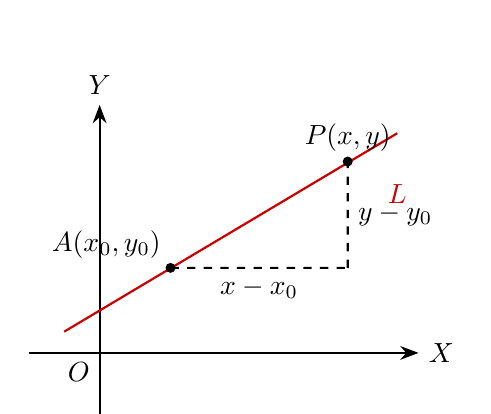
\begin{tikzpicture}[>=Stealth, scale=0.9]
  \draw[->, thick] (-1,0) -- (4.5,0) node[right] {$X$};
  \draw[->, thick] (0,-1) -- (0,3.5) node[above] {$Y$};
  \node[below left] at (0,0) {$O$};
  
  \coordinate (A) at (1.0, 1.2);
  \coordinate (P) at (3.5, 2.7);
  \draw[thick, red!80!black] (-0.5, 0.3) -- (4.2, 3.1) node[below=15pt] {$L$};
  \fill (A) circle (2pt) node[above left] {$A(x_0, y_0)$};
  \fill (P) circle (2pt) node[above] {$P(x,y)$};
  
  \draw[dashed, thick] (A) -- (3.5, 1.2) node[midway, below] {$x - x_0$};
  \draw[dashed, thick] (3.5, 1.2) -- (P) node[midway, right] {$y - y_0$};
\end{tikzpicture}
\caption{直線點斜式}
\label{fig:4-19}
\end{figure}

當 $P = A$ 時 $x = x_0$，同時 $y = y_0$，故 \eqref{eq:b3-4-11} 式自行滿足，因此 \eqref{eq:b3-4-11} 式是 $L$ 的方程式，稱 \eqref{eq:b3-4-11} 式為直線的點斜式。其實這樣的式子並不須記憶，只須了解：“左端 $L$ 上 $y$ 成分的變化 $y - y_0$ 為 $L$ 上 $x$ 成分的相應變化 $x - x_0$ 之 $m$ 倍”正是斜率 $m$ 的意義。

\begin{example}[例 11]
過點 $(2, -6)$，斜率為 $-2$ 之直線方程式為
\[ y - (-6) = -2(x - 2). \qedhere \]
\end{example}

\begin{example}[例 12]
若一直線通過點 $(-2, 2)$，且與兩座標軸所成之三角形的面積為 1，試求其方程式。
\end{example}

\begin{proof}[解]
該直線方程式因通過 $(-2, 2)$ 點，應可寫成
\[ y - 2 = m(x + 2) \]
其中 $m$ 將由該直線與兩軸圍成面積為 1 的三角形這一條件決定。

令 $y = 0$ 得直線在 $X$ 軸截距為
\[ x = -\frac{2(m+1)}{m} \]
令 $x = 0$ 得直線在 $Y$ 軸截距為
\[ y = 2(m + 1) \]
由假設知
\[ \frac{1}{2} \cdot \left| -\frac{2(m+1)}{m} \right| \cdot |2(m+1)| = 1 \]
整理得
\[ 2m^2 + 5m + 2 = 0 \]
$m = -2$ 或 $-\frac{1}{2}$。故直線方程式為
\[ 2x + y + 2 = 0 \quad\text{或}\quad x + 2y - 2 = 0. \qedhere \]
\end{proof}

\begin{figure}[H]
\centering
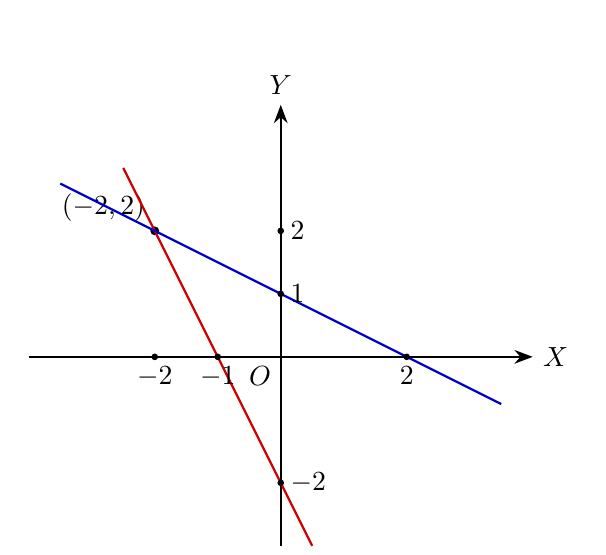
\begin{tikzpicture}[>=Stealth, scale=0.8]
  \draw[->, thick] (-4,0) -- (4,0) node[right] {$X$};
  \draw[->, thick] (0,-3) -- (0,4) node[above] {$Y$};
  \node[below left] at (0,0) {$O$};
  
  \coordinate (P) at (-2,2);
  \fill (P) circle (2pt) node[above left] {$(-2, 2)$};
  
  % Line 1: m = -2, 2x + y + 2 = 0 -> y = -2x - 2
  % Intercepts: (-1, 0), (0, -2)
  \draw[thick, red!80!black] (-2.5, 3) -- (0.5, -3) node[below] {};
  % Line 2: m = -1/2, x + 2y - 2 = 0 -> y = -0.5x + 1
  % Intercepts: (2, 0), (0, 1)
  \draw[thick, blue!80!black] (-3.5, 2.75) -- (3.5, -0.75) node[below] {};
  
  \fill (-1,0) circle (1.5pt) node[below] {$-1$};
  \fill (0,-2) circle (1.5pt) node[right] {$-2$};
  \fill (2,0) circle (1.5pt) node[below] {$2$};
  \fill (0,1) circle (1.5pt) node[right] {$1$};
  \fill (-2,0) circle (1.5pt) node[below] {$-2$};
  \fill (0,2) circle (1.5pt) node[right] {$2$};
\end{tikzpicture}
\caption{通過 $(-2,2)$ 且圍成面積為 1 的兩條直線}
\label{fig:4-20}
\end{figure}

\subsubsection*{作業 12}
\begin{enumerate}[label=(\roman*), leftmargin=2em]
  \item 試求
  \begin{enumerate}[label=(\alph*), leftmargin=2em]
    \item 過點 $(-1, 7)$，斜率為 $-\frac{1}{2}$。
    \item 過點 $(-2, 7)$，斜率為 3。
  \end{enumerate}
  之直線方程式，並繪圖示之。
  \item 若根據一正交座標系 $(O; \mathbf{e}_1, \mathbf{e}_2)$，取 $\tilde{\mathbf{e}}_1 = (1, 1), \tilde{\mathbf{e}}_2 = (0, 1)$。試求例 11 中之直線相關於 $(O; \tilde{\mathbf{e}}_1, \tilde{\mathbf{e}}_2)$ 座標之 $Y$ 對 $X$ 之變化率。
  \item 一直線過 $4x - y + 18 = 0$ 與 $6x + 7y - 42 = 0$ 之交點，而在第一象限所成之三角形面積為 72，求此直線方程式。
\end{enumerate}

\subsubsection*{習題 4-2}

\begin{enumerate}[label=\arabic*., leftmargin=2em]
  \item 給向量 $\mathbf{a} = \vec{OA}$ 及 $\mathbf{b} = \vec{OB}$，試寫出過 $A, B$ 點的直線參數式。
  \begin{enumerate}[label=(\roman*), leftmargin=2em]
    \item $A = (2, 5), B = (1, 3)$
    \item $A = (3, -1), B = (1, 2)$
    \item $A = (-1, 1), B = (2, 0)$
  \end{enumerate}
  
  \item 在正交座標系中，求適合下列各條件之直線。
  \begin{enumerate}[label=(\roman*), leftmargin=2em]
    \item 過 $(3, 5), (-3, 2)$。
    \item $X$ 截距為 2，$Y$ 截距為 5。
    \item 過 $(0, 0)$ 點，斜率為 2。
    \item $Y$ 截距為 3，斜率為 $-\frac{1}{2}$。
    \item 斜率為 3，$Y$ 截距為 6。
    \item 斜率為 $-\frac{1}{2}$，過 $(2, 3)$。
    \item 過 $(1, 7)$ 和 $(5, 6)$。
    \item 過 $(-1, 1)$，$X$ 截距為 $-2$。
  \end{enumerate}
  
  \item 設三角形三頂點為 $A(0, 0), B(0, 2), C(1, 3)$，試求
  \begin{enumerate}[label=(\roman*), leftmargin=2em]
    \item 三角形的面積
    \item 各邊方程式
    \item 三中線方程式
  \end{enumerate}
  
  \item 設一四邊形之四頂點為 $(5, 3), (8, 3), (4, 4), (7, 4)$，試求其對角線之交點。
  
  \item 設三角形三頂點之座標為 $(x_1, y_1), (x_2, y_2), (x_3, y_3)$，則其重心之座標為
  \[ \left( \frac{x_1 + x_2 + x_3}{3}, \frac{y_1 + y_2 + y_3}{3} \right) \]
  從這裏可以看出重心座標為頂點座標的平均。
  
  \item 在正交座標系中求下列各直線之斜率，$X$ 截距，$Y$ 截距，並繪其圖形。
  \begin{enumerate}[label=(\roman*), leftmargin=2em]
    \item $x + 2y = 4$
    \item $x + 2y = 2$
    \item $x + y = 0$
    \item $3x + 4y + 8 = 0$
  \end{enumerate}
  
  \item 在正交座標系中，設直線 $L$ 的傾斜角為 $\alpha$（意義如圖 \ref{fig:4-21} 所示）試說明它的斜率就是 $\tan\alpha$。
  
  \begin{figure}[H]
  \centering
  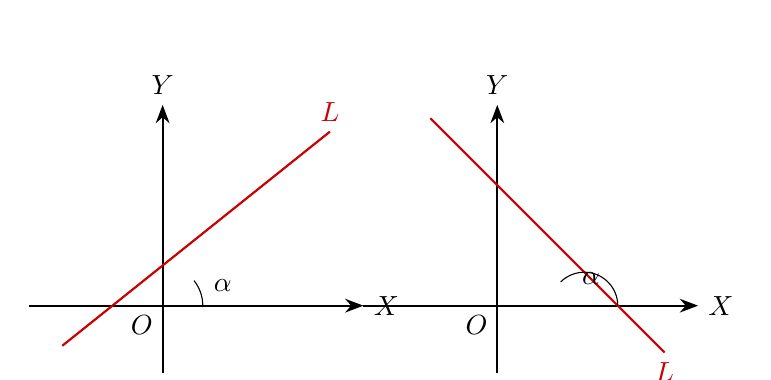
\begin{tikzpicture}[>=Stealth, scale=0.85]
    % Left: acute alpha
    \begin{scope}[shift={(0,0)}]
      \draw[->, thick] (-2,0) -- (3,0) node[right] {$X$};
      \draw[->, thick] (0,-1) -- (0,3) node[above] {$Y$};
      \node[below left] at (0,0) {$O$};
      \draw[thick, red!80!black] (-1.5, -0.6) -- (2.5, 2.6) node[above] {$L$};
      \draw (0.6,0) arc (0:38.6:0.6);
      \node at (0.9, 0.3) {$\alpha$};
    \end{scope}
    
    % Right: obtuse alpha
    \begin{scope}[shift={(5,0)}]
      \draw[->, thick] (-2,0) -- (3,0) node[right] {$X$};
      \draw[->, thick] (0,-1) -- (0,3) node[above] {$Y$};
      \node[below left] at (0,0) {$O$};
      \draw[thick, red!80!black] (-1, 2.8) -- (2.5, -0.7) node[below] {$L$};
      \draw (1.8,0) arc (0:135:0.5);
      \node at (1.4, 0.4) {$\alpha$};
    \end{scope}
  \end{tikzpicture}
  \caption{直線傾斜角 $\alpha$}
  \label{fig:4-21}
  \end{figure}
  
  \item 設 $P = (1, 2, 4), Q = (-3, -1, 0)$，且線段 $PQ$ 上有點 $M$ 到 $P$ 為到 $Q$ 距離的 5 倍，亦即
  \begin{equation}
  \overline{MP} : \overline{MQ} = 5 : 1
  \tag{A}
  \end{equation}
  \begin{enumerate}[label=(\alph*), leftmargin=2em]
    \item 求 $M$ 點之座標
  \end{enumerate}
  如果讓 $M$ 可移到 $PQ$ 延長線上
  \begin{enumerate}[label=(\alph*), leftmargin=2em, resume]
    \item 是否另外還有滿足 (A) 式的點 $M$？（若有則求出它的座標）
  \end{enumerate}
\end{enumerate}

\subsection{* 直線的一般方程}
\label{sec:4-3}

現在利用參數式及兩點式來看 § 4-1 中定理 \ref{thm:b3-4-1} 怎麼會成立的，本節亦可酌情略去。為清楚方便起見，再把定理重抄一次。

\begin{theorem*}[定理 1 重述]
\begin{enumerate}[label=(\Roman*), leftmargin=2em]
  \item 取定一個一般的座標系 $(O; \tilde{\mathbf{e}}_1, \tilde{\mathbf{e}}_2)$，一次方程式
  （假定 $a$ 與 $b$ 不全為 0），
  \begin{equation}
  ax + by + c = 0
  \tag{4}
  \end{equation}
  的軌跡一定是直線。
  \item 反過來，給了一條直線必可找到適當的 $a, b, c$，使得 (4) 式的軌跡正好是這條給定的直線。
  \item 兩個一次方程式：
  \[ a_1 x + b_1 y + c_1 = 0 \quad\text{及}\quad a_2 x + b_2 y + c_2 = 0 \]
  代表同一直線的充要條件則是存在一實數 $k \neq 0$ 使得
  \[ a_1 = k a_2, \quad b_1 = k b_2, \quad c_1 = k c_2 \]
  即：所有對應係數成比例。
\end{enumerate}
\end{theorem*}

\begin{proof}[證明]
\begin{enumerate}[label=(\Roman*), leftmargin=2em]
  \item 已給一個一次方程式
  \[ ax + by + c = 0 \quad\text{（假設 $a$ 與 $b$ 不全為 0）} \]
  欲證明其軌跡恰好為一條直線。
  
  因 $a$ 與 $b$ 不全為 0，不妨假設 $b \neq 0$。（如果是 $b = 0$ 而 $a \neq 0$，則只要把以下討論中的 $a$ 與 $b$，$x$ 與 $y$ 互換即可。）
  
  此時隨便取出兩相異實數 $x_1$ 與 $x_2$，則可解得對應之 $y_1, y_2$。
  亦即：
  \begin{equation}
  y_1 = -\frac{a x_1 + c}{b}, \quad y_2 = -\frac{a x_2 + c}{b}
  \label{eq:b3-4-12}
  \end{equation}
  而兩點 $A(x_1, y_1), B(x_2, y_2)$ 應為滿足 $ax + by + c = 0$ 之兩個相異點，此因 \eqref{eq:b3-4-12} 式給出了
  \begin{equation}
  \begin{cases}
  a x_1 + b y_1 + c = 0 \\
  a x_2 + b y_2 + c = 0
  \end{cases}
  \label{eq:b3-4-13}
  \end{equation}
  
  \begin{figure}[H]
  \centering
  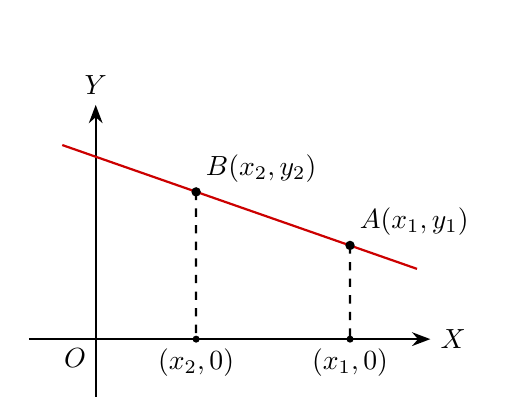
\begin{tikzpicture}[>=Stealth, scale=0.85]
    \draw[->, thick] (-1,0) -- (5,0) node[right] {$X$};
    \draw[->, thick] (0,-1) -- (0,3.5) node[above] {$Y$};
    \node[below left] at (0,0) {$O$};
    
    \coordinate (B) at (1.5, 2.2);
    \coordinate (A) at (3.8, 1.4);
    \draw[thick, red!80!black] (-0.5, 2.9) -- (4.8, 1.05);
    \fill (A) circle (2pt) node[above right] {$A(x_1, y_1)$};
    \fill (B) circle (2pt) node[above right] {$B(x_2, y_2)$};
    
    \draw[dashed, thick] (A) -- (3.8, 0);
    \draw[dashed, thick] (B) -- (1.5, 0);
    \fill (3.8, 0) circle (1.5pt) node[below] {$(x_1, 0)$};
    \fill (1.5, 0) circle (1.5pt) node[below] {$(x_2, 0)$};
  \end{tikzpicture}
  \caption{一次方程式直線軌跡}
  \label{fig:4-22}
  \end{figure}
  
  設 $L$ 為由 $A$ 與 $B$ 決定出來的直線，由直線座標參數式 \eqref{eq:b3-4-6}，
  \[ \begin{cases} x = x_1 + t(x_2 - x_1) \\ y = y_1 + t(y_2 - y_1) \end{cases} \]
  馬上可以推知點 $P(x, y)$ 滿足一次式 $ax + by + c = 0$。
  
  反過來 $ax + by + c = 0$ 上的點，也一定要在 $L$ 上。道理是這樣：
  若 $P(x, y)$ 滿足 $ax + by + c = 0$，則由 \eqref{eq:b3-4-13} 式可得
  \begin{align*}
  -a(x - x_1) &= b(y - y_1) \\
  -b(y_2 - y_1) &= a(x_2 - x_1)
  \end{align*}
  故當 $a \neq 0$ 時，上兩式相乘，移項得
  \[ (x - x_1)(y_2 - y_1) - (y - y_1)(x_2 - x_1) = 0 \]
  由兩點式中的討論知 $P(x, y)$ 就在 $L$ 上。
  
  如果 $a = 0$，則 $y = -\frac{c}{b}$，而由 \eqref{eq:b3-4-13} 式 $y_1, y_2$ 亦皆等於 $-\frac{c}{b}$，$L$ 為 $y$ 座標等於 $-\frac{c}{b}$ 而平行於 $X$ 軸的直線，故 $P(x, -\frac{c}{b})$ 即在 $L$ 上，見圖 \ref{fig:4-23}。
  
  \begin{figure}[H]
  \centering
  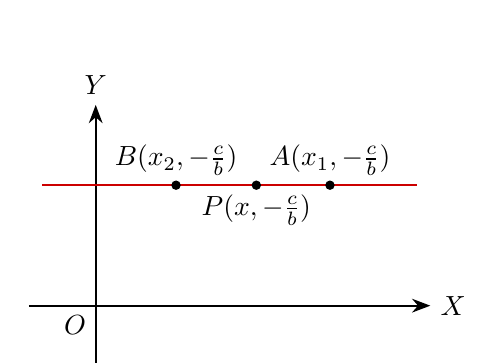
\begin{tikzpicture}[>=Stealth, scale=0.85]
    \draw[->, thick] (-1,0) -- (5,0) node[right] {$X$};
    \draw[->, thick] (0,-1) -- (0,3) node[above] {$Y$};
    \node[below left] at (0,0) {$O$};
    
    \draw[thick, red!80!black] (-0.8, 1.8) -- (4.8, 1.8);
    \coordinate (B) at (1.2, 1.8);
    \coordinate (A) at (3.5, 1.8);
    \coordinate (P) at (2.4, 1.8);
    \fill (A) circle (2pt) node[above] {$A(x_1, -\frac{c}{b})$};
    \fill (B) circle (2pt) node[above] {$B(x_2, -\frac{c}{b})$};
    \fill (P) circle (2pt) node[below] {$P(x, -\frac{c}{b})$};
  \end{tikzpicture}
  \caption{$a=0$ 時平行於 $X$ 軸之直線}
  \label{fig:4-23}
  \end{figure}
  
  \item 欲證明任給一條直線，必可表為某一一次方程式 $ax + by + c = 0$ 的軌跡。
  
  其實兩點式的討論中已證明出這件事，因給了一條直線，可挑出相異兩點 $A(x_1, y_1), B(x_2, y_2)$，由前所述知此直線正好是
  \[ (x - x_1)(y_2 - y_1) - (y - y_1)(x_2 - x_1) = 0 \]
  的軌跡。
  
  將此兩點式展開後集項，得
  \[ (y_2 - y_1)x - (x_2 - x_1)y + (x_2 y_1 - x_1 y_2) = 0 \]
  只將式中三個係數分別取為 $a, b, c$，便為所求。
  
  \item 若 $a_1 x + b_1 y + c_1 = 0$ 與 $a_2 x + b_2 y + c_2 = 0$ 代表同一直線，若存在 $k \neq 0$ 使 $a_1 = k a_2, b_1 = k b_2, c_1 = k c_2$，則
  \[ a_1 x + b_1 y + c_1 = k(a_2 x + b_2 y + c_2) = 0 \]
  相當於 $a_2 x + b_2 y + c_2 = 0$，故兩方程式之軌跡一模一樣。
  
  反過來，若兩式代表同一直線，則
  \[ \begin{cases} a_1 x + b_1 y + c_1 = 0 \\ a_2 x + b_2 y + c_2 = 0 \end{cases} \]
  有無窮多解。
  第一冊「一次方程組理論」告訴我們，此時必然
  \[ a_1 c_2 - a_2 c_1 = 0 \quad\text{且}\quad b_1 c_2 - b_2 c_1 = 0 \]
  亦即
  \[ a_1 : a_2 = b_1 : b_2 = c_1 : c_2. \qedhere \]
\end{enumerate}
\end{proof}

\subsubsection*{習題 4-3}

在正交座標系中，若直線 $L$ 的方程式為 $ax + by + c = 0$，試寫出 1、2、3 各式，並討論各式成立時關於 $a, b, c$ 的條件；
\begin{enumerate}[label=\arabic*., leftmargin=2em]
  \item $L$ 的 $X$ 截距，$Y$ 截距，及 $L$ 的截距式。
  \item $L$ 的斜率及 $L$ 的斜截式。
  \item $L$ 上點 $P(x, y)$ 所相應向量 $\vec{OP}$ 的參數式。
  \item 若 $L$ 過 $A(x_1, y_1), B(x_2, y_2)$ 兩點，試以 $x_1, y_1, x_2, y_2$ 表示係數之比 $a : b : c$。
\end{enumerate}

\subsection{法線式及其應用}
\label{sec:4-4}

這一整節我們局限於採用正交座標系。

\subsubsection*{甲、法線式}

與一條直線垂直的一個有向線段經過平移以後還是與該直線垂直。因此所有與這直線垂直的向量方向要麼相同，要麼指向正好相反。

給了一條直線 $L$，可作 $L$ 的一個單位法向量 $\mathbf{u}$ 使得
\[ \mathbf{u} = (\cos\omega, \sin\omega) \quad\text{〔參見 § 3-5〕} \]
而 $0 \le \omega < \pi$。這時 $\omega$ 稱為 $L$ 的法向角。

\begin{figure}[H]
\centering
\begin{subfigure}[b]{0.48\textwidth}
\centering
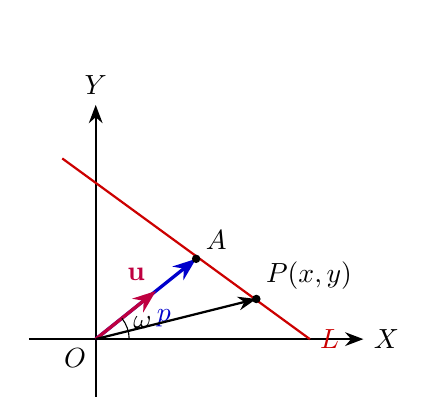
\begin{tikzpicture}[>=Stealth, scale=0.85]
  \draw[->, thick] (-1,0) -- (4,0) node[right] {$X$};
  \draw[->, thick] (0,-1) -- (0,3.5) node[above] {$Y$};
  \node[below left] at (0,0) {$O$};
  
  \coordinate (A) at (1.5, 1.2);
  \draw[thick, red!80!black] (-0.5, 2.7) -- (3.2, 0) node[right] {$L$};
  \draw[->, very thick, blue!80!black] (0,0) -- (A) node[midway, below right] {$p$};
  \fill (A) circle (1.8pt) node[above right] {$A$};
  
  \coordinate (U) at (0.9, 0.72);
  \draw[->, very thick, purple] (0,0) -- (U) node[above left] {$\mathbf{u}$};
  \draw (0.5,0) arc (0:38.6:0.5);
  \node at (0.7, 0.25) {$\omega$};
  
  \coordinate (P) at (2.4, 0.6);
  \draw[->, thick] (0,0) -- (P);
  \fill (P) circle (1.8pt) node[above right] {$P(x,y)$};
\end{tikzpicture}
\caption{$p > 0$（$\mathbf{u}$ 與 $\vec{OA}$ 同向）}
\label{fig:4-24-a}
\end{subfigure}
\hfill
\begin{subfigure}[b]{0.48\textwidth}
\centering
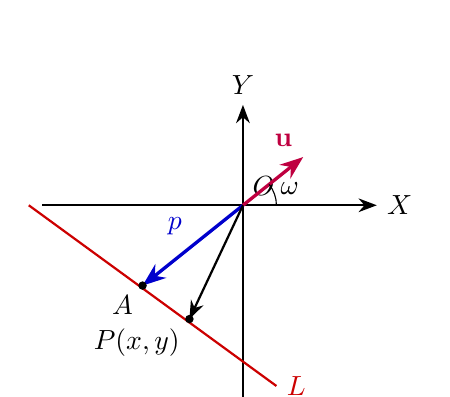
\begin{tikzpicture}[>=Stealth, scale=0.85]
  \draw[->, thick] (-3,0) -- (2,0) node[right] {$X$};
  \draw[->, thick] (0,-3) -- (0,1.5) node[above] {$Y$};
  \node[above right] at (0,0) {$O$};
  
  \coordinate (A) at (-1.5, -1.2);
  \draw[thick, red!80!black] (-3.2, 0) -- (0.5, -2.7) node[right] {$L$};
  \draw[->, very thick, blue!80!black] (0,0) -- (A) node[midway, above left] {$p$};
  \fill (A) circle (1.8pt) node[below left] {$A$};
  
  \coordinate (U) at (0.9, 0.72);
  \draw[->, very thick, purple] (0,0) -- (U) node[above left] {$\mathbf{u}$};
  \draw (0.5,0) arc (0:38.6:0.5);
  \node at (0.7, 0.25) {$\omega$};
  
  \coordinate (P) at (-0.8, -1.7);
  \draw[->, thick] (0,0) -- (P);
  \fill (P) circle (1.8pt) node[below left] {$P(x,y)$};
\end{tikzpicture}
\caption{$p < 0$（$\mathbf{u}$ 與 $\vec{OA}$ 異向）}
\label{fig:4-24-b}
\end{subfigure}
\caption{直線法向角與帶號距離}
\label{fig:4-24}
\end{figure}

設 $p$ 為這樣的一個實數：其絕對值為自原點到 $L$ 的距離。當 $L$ 經過點 $O$ 時，$p = 0$，當 $L$ 不經過 $O$ 時，由 $O$ 向 $L$ 引一垂線 $\vec{OA}$，其中 $A$ 為垂足，而定義：
\begin{align*}
p &> 0；\quad\text{若 $\mathbf{u}$ 與 $\vec{OA}$ 同向（如圖 \ref{fig:4-24-a}）} \\
p &< 0；\quad\text{若 $\mathbf{u}$ 與 $\vec{OA}$ 異向（如圖 \ref{fig:4-24-b}）}
\end{align*}
以下我們要來看看，若已知 $\omega$ 角及 $p$，如何表出直線 $L$ 的方程式。反過來，如果已知一個一次方程式為：
\[ ax + by + c = 0 \]
可否求得其法線式。

設 $P(x, y)$ 為直線上任意點，由內積的幾何意義知
\[ \vec{OP}\cdot\mathbf{u} = \vec{OP} \text{ 在 } \mathbf{u} \text{ 方向的投影量} = p \]
但 $\vec{OP} = (x, y), \mathbf{u} = (\cos\omega, \sin\omega)$，故由內積定義知
\begin{equation}
(\cos\omega)x + (\sin\omega)y = p
\label{eq:b3-4-14}
\end{equation}
這式稱為 $L$ 的法線式〔每寫下這法線式時，應清楚知道它的幾何意義：左端是 $\vec{OP}$ 在 $\mathbf{u}$ 方向的投影量，右端則是 $O$ 到直線 $L$ 的帶號（可正可負）的距離〕。

反過來，給定一個一次方程式
\begin{equation}
ax + by + c = 0
\label{eq:b3-4-15}
\end{equation}
它代表的軌跡，由定理 \ref{thm:b3-4-1} 已知為一直線，故由上述討論知可表成法線式
\begin{equation}
(\cos\omega)x + (\sin\omega)y - p = 0
\label{eq:b3-4-16}
\end{equation}
由於這兩式 \eqref{eq:b3-4-15}, \eqref{eq:b3-4-16} 代表同一直線，其對應係數應成比例，故存在一適當 $k \neq 0$，使
\[ a = k\cos\omega, \quad b = k\sin\omega, \quad c = -kp \]
但
\[ a^2 + b^2 = k^2(\cos^2\omega + \sin^2\omega) = k^2 \]
故求得
\begin{equation}
k = \pm\sqrt{a^2 + b^2}
\label{eq:b3-4-17}
\end{equation}
而
\[ \cos\omega = \frac{a}{\pm\sqrt{a^2 + b^2}}, \quad \sin\omega = \frac{b}{\pm\sqrt{a^2 + b^2}}, \quad p = \frac{-c}{\pm\sqrt{a^2 + b^2}} \]
其中 $\pm$ 的調整是基於 $0 \le \omega < \pi$ 這已固定的選擇而定。換句話說，由於 $\sin\omega \ge 0$，故分母的符號應與 $b$ 的符號一致（若 $b = 0$，則分母符號與 $a$ 一致）。

\begin{example}[例 13]
設 $L : 3x + 4y - 10 = 0$，則其夾角限制在 $0$ 與 $\pi$ 之間的單位法向量 $\mathbf{u}$ 之座標為
\[ \mathbf{u} = \left(\frac{3}{\sqrt{3^2+4^2}}, \frac{4}{\sqrt{3^2+4^2}}\right) = \left(\frac{3}{5}, \frac{4}{5}\right) \]
故 $\cos\omega = \frac{3}{5}, \sin\omega = \frac{4}{5}$（即 $\omega$ 約為 $53^\circ 8'$），$p = \frac{10}{5} = 2$。
\end{example}

\begin{figure}[H]
\centering
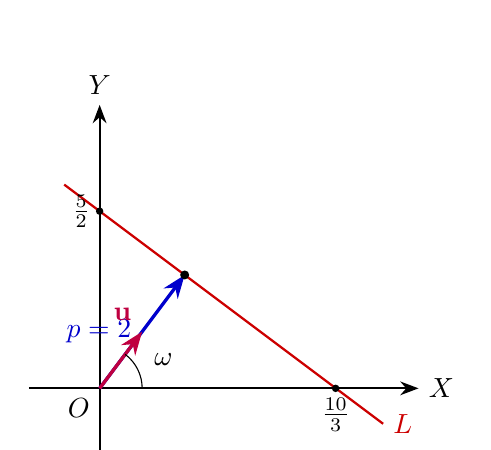
\begin{tikzpicture}[>=Stealth, scale=0.9]
  \draw[->, thick] (-1,0) -- (4.5,0) node[right] {$X$};
  \draw[->, thick] (0,-1) -- (0,4) node[above] {$Y$};
  \node[below left] at (0,0) {$O$};
  
  % 3x + 4y - 10 = 0 => x=10/3=3.33, y=2.5
  \coordinate (A) at (1.2, 1.6);
  \draw[thick, red!80!black] (-0.5, 2.875) -- (4.0, -0.5) node[right] {$L$};
  \draw[->, very thick, blue!80!black] (0,0) -- (A) node[midway, left] {$p=2$};
  \fill (A) circle (1.8pt);
  
  \coordinate (U) at (0.6, 0.8);
  \draw[->, very thick, purple] (0,0) -- (U) node[above left] {$\mathbf{u}$};
  \draw (0.6,0) arc (0:53.13:0.6);
  \node at (0.9, 0.4) {$\omega$};
  
  \fill (3.33,0) circle (1.5pt) node[below] {$\frac{10}{3}$};
  \fill (0,2.5) circle (1.5pt) node[left] {$\frac{5}{2}$};
\end{tikzpicture}
\caption{直線 $3x+4y-10=0$ 之法線式}
\label{fig:4-25}
\end{figure}

\begin{example}[例 14]
直線 $5x + 2 = 0$ 之法線式為
\[ 1\cdot x + 0\cdot y = -\frac{2}{5} \]
得 $\cos\omega = 1, \sin\omega = 0$，而 $p = -\frac{2}{5}$。此時 $\omega = 0$。
\end{example}

\subsubsection*{作業 13}
試寫出下列各式之法線式，並定出 $\omega$ 及 $p$。
\begin{enumerate}[label=(\roman*), leftmargin=2em]
  \item $2x + 5y + 3 = 0$
  \item $4x + 2y - 1 = 0$
  \item $x + y + 1 = 0$
  \item $10x + 5 = 0$
\end{enumerate}

\subsubsection*{乙、直線方向及直線交角}

給定一直線 $L : ax + by + c = 0$，設 $\omega$ 為 $L$ 的法向角，而 $\mathbf{u} = (\cos\omega, \sin\omega)$。今規定 $L$ 之方向為：
將 $\mathbf{u}$ 依順時針方向（負向）轉 $\frac{\pi}{2}$ 後的方向。
由圖易知自 $X$ 軸轉到 $L$ 之角的角度為 $\theta = \omega - \frac{\pi}{2}$（可正可負）。

\begin{figure}[H]
\centering
\begin{subfigure}[b]{0.48\textwidth}
\centering
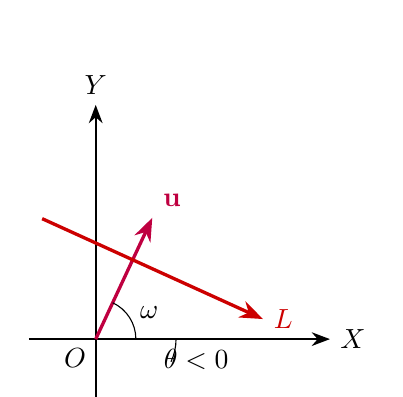
\begin{tikzpicture}[>=Stealth, scale=0.85]
  \draw[->, thick] (-1,0) -- (3.5,0) node[right] {$X$};
  \draw[->, thick] (0,-1) -- (0,3.5) node[above] {$Y$};
  \node[below left] at (0,0) {$O$};
  
  \draw[->, very thick, purple] (0,0) -- (65:2) node[above right] {$\mathbf{u}$};
  \draw (0.6,0) arc (0:65:0.6);
  \node at (0.8,0.4) {$\omega$};
  
  % L perpendicular to u, directed along omega - 90 = -25 deg
  \draw[->, very thick, red!80!black] (-0.8, 1.8) -- (2.5, 0.3) node[right] {$L$};
  \draw (1.2,0) arc (0:-25:0.8);
  \node at (1.5, -0.3) {$\theta < 0$};
\end{tikzpicture}
\caption{$\omega > \frac{\pi}{2}$ 時，$\theta < 0$}
\label{fig:4-26-1}
\end{subfigure}
\hfill
\begin{subfigure}[b]{0.48\textwidth}
\centering
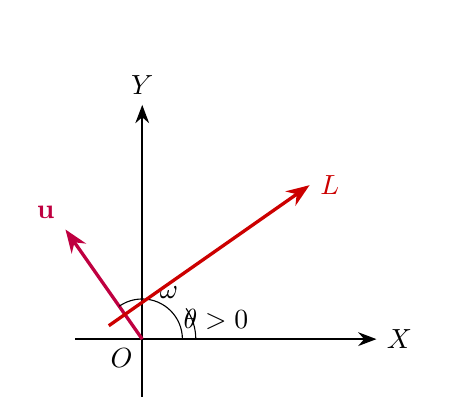
\begin{tikzpicture}[>=Stealth, scale=0.85]
  \draw[->, thick] (-1,0) -- (3.5,0) node[right] {$X$};
  \draw[->, thick] (0,-1) -- (0,3.5) node[above] {$Y$};
  \node[below left] at (0,0) {$O$};
  
  \draw[->, very thick, purple] (0,0) -- (125:2) node[above left] {$\mathbf{u}$};
  \draw (0.6,0) arc (0:125:0.6);
  \node at (0.4,0.7) {$\omega$};
  
  % L directed along omega - 90 = 35 deg
  \draw[->, very thick, red!80!black] (-0.5, 0.2) -- (2.5, 2.3) node[right] {$L$};
  \draw (0.8,0) arc (0:35:0.8);
  \node at (1.1, 0.3) {$\theta > 0$};
\end{tikzpicture}
\caption{$\omega < \frac{\pi}{2}$ 時，$\theta > 0$}
\label{fig:4-26-2}
\end{subfigure}
\caption{有向直線的方向規定}
\label{fig:4-26}
\end{figure}

這樣帶有方向的直線稱為有向直線，在座標面上容易看出我們以上所規定的直線的方向便是直線上點之橫座標漸增的方向。

對於一條直線 $L$ 的方程式 $ax + by + c = 0$，我們可以調整其間係數，使得
\[ b \ge 0 \quad\text{且若 $b = 0$ 時，$a \ge 0$} \]
〔必要時，可在 $ax + by + c = 0$ 的兩端各乘以 $-1$ 而改變 $b$ 或 $a$ 的性質符號〕。

經過這樣的調整以後，上述根據法向角 $\omega$ 選定的單位法向量 $\mathbf{u}$ 便與向量 $(a, b)$ 同方向。此時，
\[ \mathbf{u} = \frac{(a, b)}{\sqrt{a^2 + b^2}} \]

\subsubsection*{作業 14}
設有一直線，其 $X$ 截距為 2，且斜率為 $-1$，試寫出它的方程式，並繪圖表示這直線依照上述規定的方向。

今設兩直線 $L_1$ 及 $L_2$ 的法向角分別為 $\omega_1$ 及 $\omega_2$，而取單位法向量
\[ \mathbf{u}_1 = (\cos\omega_1, \sin\omega_1), \quad \mathbf{u}_2 = (\cos\omega_2, \sin\omega_2) \]
我們根據上述，調整
\begin{align*}
L_1 &: a_1 x + b_1 y + c_1 = 0 \\
L_2 &: a_2 x + b_2 y + c_2 = 0
\end{align*}
中的係數 $a_1, b_1, c_1$ 與 $a_2, b_2, c_2$，使得 $\mathbf{u}_1$ 與 $\mathbf{u}_2$ 分別與向量 $(a_1, b_1), (a_2, b_2)$ 同向，而得
\[ \mathbf{u}_1 = \frac{(a_1, b_1)}{\sqrt{a_1^2 + b_1^2}}, \quad \mathbf{u}_2 = \frac{(a_2, b_2)}{\sqrt{a_2^2 + b_2^2}} \]
依上述規定 $L_1, L_2$ 各有了方向後的有向直線必要時分別記成 $\vec{L}_1, \vec{L}_2$。欲求 $\vec{L}_1$ 繞到 $\vec{L}_2$ 的轉角角度 $\theta$，〔限制在 $-\frac{\pi}{2}$ 與 $\frac{\pi}{2}$ 之間〕。

設 $\theta_1, \theta_2$ 分別為 $\vec{L}_1, \vec{L}_2$ 的“傾斜角”〔有向直線 $\vec{L}$ 的“傾斜角”指 $OX$ 到 $\vec{L}$ 方向的轉角。角度限制在 $-\frac{\pi}{2}$ 到 $\frac{\pi}{2}$ 之間〕。

\begin{figure}[H]
\centering
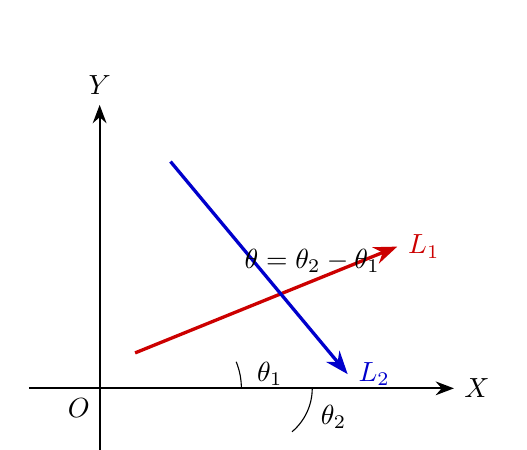
\begin{tikzpicture}[>=Stealth, scale=0.9]
  \draw[->, thick] (-1,0) -- (5,0) node[right] {$X$};
  \draw[->, thick] (0,-1) -- (0,4) node[above] {$Y$};
  \node[below left] at (0,0) {$O$};
  
  % L1 line
  \draw[->, very thick, red!80!black] (0.5, 0.5) -- (4.2, 2.0) node[right] {$L_1$};
  % L2 line
  \draw[->, very thick, blue!80!black] (1.0, 3.2) -- (3.5, 0.2) node[right] {$L_2$};
  
  \draw (2.0,0) arc (0:22:1.0);
  \node at (2.4, 0.2) {$\theta_1$};
  \draw (3.0,0) arc (0:-50:0.8);
  \node at (3.3, -0.4) {$\theta_2$};
  
  \node at (3.0, 1.8) {$\theta = \theta_2 - \theta_1$};
\end{tikzpicture}
\caption{兩直線交角}
\label{fig:4-27}
\end{figure}

則
\[ \theta_1 = \omega_1 - \frac{\pi}{2}, \quad \theta_2 = \omega_2 - \frac{\pi}{2} \]
故
\[ \theta = \theta_2 - \theta_1 = \omega_2 - \omega_1 \]
故
\[ \cos\theta = \cos(\omega_2 - \omega_1) = \mathbf{u}_1\cdot\mathbf{u}_2 = \frac{a_1 a_2 + b_1 b_2}{\sqrt{a_1^2 + b_1^2}\sqrt{a_2^2 + b_2^2}} \]
轉角角度 $\theta$ 便可由三角函數表查得。

由此我們順便得到 $L_1 \parallel L_2$ 及 $L_1 \perp L_2$ 的充要條件。
〔注意 我們規定兩直線重合也看成是平行的一個特殊情形〕

\begin{proposition}
\label{prop:b3-4-1}
兩直線 $L_1 : a_1 x + b_1 y + c_1 = 0, L_2 : a_2 x + b_2 y + c_2 = 0$ 平行的充要條件是
\begin{equation}
a_1 : b_1 = a_2 : b_2
\label{eq:b3-4-19}
\end{equation}
（即當兩線之斜率有定義時，兩斜率 $m_1 = m_2$，注意 $m_i = -\frac{a_i}{b_i}$），亦即
\[ a_1 b_2 - a_2 b_1 = 0 \]
而 $L_1$ 與 $L_2$ 直交的充要條件則為
\begin{equation}
a_1 a_2 + b_1 b_2 = 0 \quad\text{〔即 $m_1 \cdot m_2 = -1$〕}
\label{eq:b3-4-20}
\end{equation}
\end{proposition}

\begin{proof}[證明]
$L_1 \parallel L_2$ 的充要條件是 $\theta = 0$ 或 $\cos\theta = 1$，亦即
\[ \frac{a_1 a_2 + b_1 b_2}{\sqrt{a_1^2 + b_1^2}\sqrt{a_2^2 + b_2^2}} = 1 \]
〔注意這便是柯西-舒瓦茲不等式退化為等式的情形〕，即 $(a_1 b_2 - a_2 b_1)^2 = 0$，即 $a_1 b_2 - a_2 b_1 = 0$。得證。

另一命題：$L_1 \perp L_2$ 的充要條件是 $\theta = \frac{\pi}{2}$ 或 $\cos\theta = 0$，亦即 $a_1 a_2 + b_1 b_2 = 0$。
\end{proof}

\paragraph*{注意}
比較直截地了解這直線平行或垂直的充要條件的方法是去注意下面一件事：向量 $(a, b)$ 為直線 $L : ax + by + c = 0$ 的“法向量”〔即垂直於 $L$ 的一個向量〕。又，$L_1$ 與 $L_2$ 平行或垂直的充要條件是其相應法向量為平行或垂直，即：
\[ L_1 \parallel L_2 \iff (a_1, b_1) \parallel (a_2, b_2) \iff a_1 : b_1 = a_2 : b_2 \]
而
\[ L_1 \perp L_2 \iff (a_1, b_1)\cdot(a_2, b_2) = 0 \iff a_1 a_2 + b_1 b_2 = 0. \]

\begin{example}[例 15]
求一通過 $(1, 2)$ 點且與直線 $2x + y = 1$
\begin{enumerate}[label=(\roman*), leftmargin=2em]
  \item 平行，或
  \item 直交
\end{enumerate}
的直線方程式。
\end{example}

\begin{proof}[解]
\begin{enumerate}[label=(\roman*), leftmargin=2em]
  \item 設所求為 $ax + by + c = 0$（$a, b$ 不全為零），則根據命題 \ref{prop:b3-4-1}，
  \[ \frac{a}{2} = \frac{b}{1} \implies a - 2b = 0 \quad\dots\dots (21) \]
  但因通過點 $(1, 2)$，以之代入 $ax + by + c = 0$ 中，可得
  \[ a + 2b + c = 0 \quad\dots\dots (22) \]
  解 (21) 及 (22) 得 $a = 2b, 4b + c = 0 \implies c = -4b$。故得 $2bx + by - 4b = 0 \implies 2x + y - 4 = 0$（因 $b \neq 0$）。
  
  \item 設所求為 $ax + by + c = 0$，則由垂直條件
  \[ 2a + b = 0 \quad\dots\dots (23) \]
  又通過點 $(1, 2)$，
  \[ a + 2b + c = 0 \quad\dots\dots (24) \]
  解 (23) 及 (24)，$b = -2a, c = 3a$。故所求方程式為 $ax - 2ay + 3a = 0 \implies x - 2y + 3 = 0$（因 $a \neq 0$）。
\end{enumerate}
\end{proof}

\begin{figure}[H]
\centering
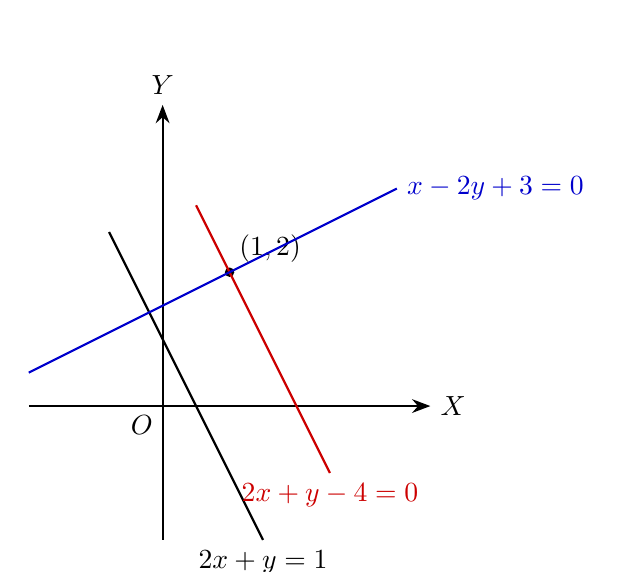
\begin{tikzpicture}[>=Stealth, scale=0.85]
  \draw[->, thick] (-2,0) -- (4,0) node[right] {$X$};
  \draw[->, thick] (0,-2) -- (0,4.5) node[above] {$Y$};
  \node[below left] at (0,0) {$O$};
  
  \coordinate (P) at (1,2);
  \fill (P) circle (2pt) node[above right] {$(1, 2)$};
  
  % Original line: 2x + y = 1 -> y = -2x + 1
  \draw[thick] (-0.8, 2.6) -- (1.5, -2) node[below] {$2x+y=1$};
  % Parallel line: 2x + y - 4 = 0 -> y = -2x + 4
  \draw[thick, red!80!black] (0.5, 3) -- (2.5, -1) node[below] {$2x+y-4=0$};
  % Perpendicular line: x - 2y + 3 = 0 -> y = 0.5x + 1.5
  \draw[thick, blue!80!black] (-2, 0.5) -- (3.5, 3.25) node[right] {$x-2y+3=0$};
\end{tikzpicture}
\caption{過 $(1,2)$ 與給定直線平行及垂直之直線}
\label{fig:4-28}
\end{figure}

\subsubsection*{作業 15}
\begin{enumerate}[label=(\roman*), leftmargin=2em]
  \item 求過點 $(2, 4)$，而與直線 $2x + y - 1 = 0$ 成 $45^\circ$ 角之直線方程式。
  \item 如圖 \ref{fig:4-29-1} 在單位圓上，求切線方程式。
  \item 如圖 \ref{fig:4-29-2} 求正立方體兩對角線的交角 $\theta$。
  〔提示：在矩形 $ABCD$ 的平面上取座標系 $(B; \mathbf{e}_1, \mathbf{e}_2)$，其中 $\mathbf{e}_1, \mathbf{e}_2$ 為與 $\vec{BA}, \vec{BC}$ 同方向的兩單位向量〕請以本節直線交角方法求之，又另以向量幾何方法求之。（後法提示：考慮 $\vec{BD}$ 與 $\vec{AC}$ 的內積）。
  \item 碳原子 C 常與四個氫原子結合如圖，中間的連線稱為它的價鍵，試求任兩價鍵間的夾角。（查表求出角度）。
\end{enumerate}

\begin{figure}[H]
\centering
\begin{subfigure}[b]{0.45\textwidth}
\centering
\begin{tikzpicture}[>=Stealth, scale=1.1]
  \draw[->, thick] (-1.5,0) -- (1.8,0) node[right] {$X$};
  \draw[->, thick] (0,-1.5) -- (0,1.8) node[above] {$Y$};
  \node[below left] at (0,0) {$O$};
  \draw[thick] (0,0) circle (1);
  \coordinate (P) at (40:1);
  \draw[thick] (0,0) -- (P);
  \fill (P) circle (1.5pt) node[above right] {$P(x_0, y_0)$};
  % Tangent line
  \draw[thick, red!80!black] ($(P) + (-50:1.3)$) -- ($(P) + (130:1.3)$);
\end{tikzpicture}
\caption{單位圓切線}
\label{fig:4-29-1}
\end{subfigure}
\hfill
\begin{subfigure}[b]{0.45\textwidth}
\centering
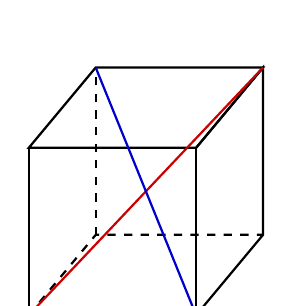
\begin{tikzpicture}[>=Stealth, scale=0.85]
  % Cube
  \coordinate (O) at (0,0);
  \coordinate (A) at (2.5,0);
  \coordinate (B) at (3.5,1.2);
  \coordinate (C) at (1.0,1.2);
  \coordinate (D) at (0,2.5);
  \coordinate (E) at (2.5,2.5);
  \coordinate (F) at (3.5,3.7);
  \coordinate (G) at (1.0,3.7);
  
  \draw[thick] (O) -- (A) -- (E) -- (D) -- cycle;
  \draw[thick] (A) -- (B) -- (F) -- (E);
  \draw[thick] (D) -- (E) -- (F) -- (G) -- cycle;
  \draw[dashed, thick] (O) -- (C) -- (B);
  \draw[dashed, thick] (C) -- (G);
  
  % Diagonals
  \draw[thick, red!80!black] (O) -- (F);
  \draw[thick, blue!80!black] (A) -- (G);
\end{tikzpicture}
\caption{正立方體對角線}
\label{fig:4-29-2}
\end{subfigure}
\caption{直線交角作業幾何圖示}
\end{figure}

\subsubsection*{丙、二元一次二式聯立方程求解的幾何解釋}

我們回頭利用座標幾何的轉化，將代數上第一冊所學的二元一次（二式）聯立方程的求解問題與幾何上兩直線之是否相交或平行的問題作一個對照。

設
\begin{equation}
\begin{cases}
a_1 x + b_1 y + c_1 = 0 \\
a_2 x + b_2 y + c_2 = 0
\end{cases}
\label{eq:b3-4-25}
\end{equation}
為一已給的聯立方程。設兩式之軌跡按序為兩直線 $L_1$ 與 $L_2$。§ 4-1 丙段中已討論過：$L_1 \cap L_2$ 其實就是 \eqref{eq:b3-4-25} 之解（或稱解集合）我們按照 $L_1, L_2$ 之幾何相關情狀來分析其相應代數條件：

\begin{figure}[H]
\centering
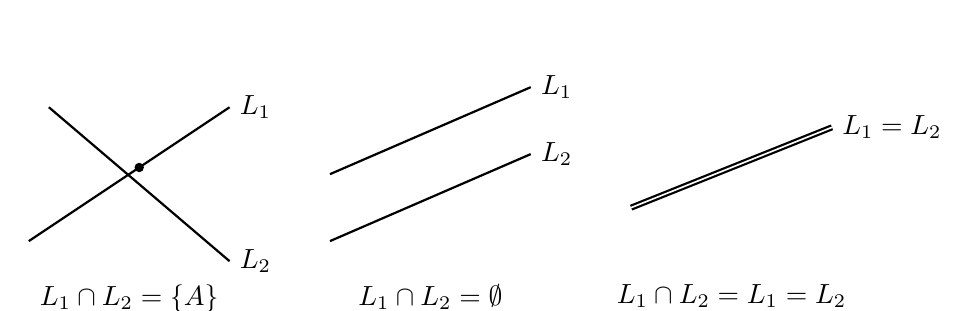
\begin{tikzpicture}[>=Stealth, scale=0.85]
  % (I) Intersecting
  \begin{scope}[shift={(0,0)}]
    \draw[thick] (-1.5,-0.5) -- (1.5,1.5) node[right] {$L_1$};
    \draw[thick] (-1.2,1.5) -- (1.5,-0.8) node[right] {$L_2$};
    \fill (0.15,0.6) circle (2pt);
    \node[below] at (0,-1) {$L_1 \cap L_2 = \{A\}$};
  \end{scope}
  
  % (II) Parallel distinct
  \begin{scope}[shift={(4.5,0)}]
    \draw[thick] (-1.5,0.5) -- (1.5,1.8) node[right] {$L_1$};
    \draw[thick] (-1.5,-0.5) -- (1.5,0.8) node[right] {$L_2$};
    \node[below] at (0,-1) {$L_1 \cap L_2 = \emptyset$};
  \end{scope}
  
  % (III) Coincident
  \begin{scope}[shift={(9,0)}]
    \draw[thick, double] (-1.5,0) -- (1.5,1.2) node[right] {$L_1 = L_2$};
    \node[below] at (0,-1) {$L_1 \cap L_2 = L_1 = L_2$};
  \end{scope}
\end{tikzpicture}
\caption{兩直線相交、平行與重合}
\label{fig:4-30}
\end{figure}

\begin{enumerate}[label=(\Roman*), leftmargin=2em]
  \item $L_1$ 與 $L_2$ 相交於一點 $\iff L_1$ 與 $L_2$ 不平行 $\iff a_1 b_2 - a_2 b_1 \neq 0$。
  \item $L_1$ 與 $L_2$ 平行 $\iff a_1 b_2 - a_2 b_1 = 0$。在平行的假設下，分兩種場合討論：
  \begin{enumerate}[label=(\roman*), leftmargin=2em]
    \item $L_1$ 與 $L_2$ 不重合：即 \eqref{eq:b3-4-25} 式無解，亦即 $L_1 \cap L_2 = \emptyset$，其代數條件如下：
    \[ a_1 : a_2 = b_1 : b_2 \neq c_1 : c_2 \quad\text{（即所謂矛盾方程組）} \]
    \item $L_1$ 與 $L_2$ 重合：即 \eqref{eq:b3-4-25} 式有無窮多解，亦即 $L_1 \cap L_2 = L_1 = L_2$，其代數條件如下：
    \[ a_1 : a_2 = b_1 : b_2 = c_1 : c_2 \quad\text{（即所謂同義方程組）} \]
  \end{enumerate}
\end{enumerate}

\subsubsection*{作業 16}
就 (I), (II)(i) 與 (II)(ii) 三類各舉一相應的聯立方程的例子，各畫出其所代表的直線，並驗證相應的代數條件。

\subsubsection*{丁、點與直線間距}

給定平面上一點 $Q(x_0, y_0)$，及一直線
\[ L : ax + by + c = 0 \]
欲求 $Q$ 點到 $L$ 之距離（即垂直距離），此距離記為 $d(Q, L)$。如法線式中所述，取
\[ \mathbf{u} = (\cos\omega, \sin\omega), \quad 0 \le \omega < \pi \]
為一個 $L$ 之單位法向量，取 $P(x, y)$ 為 $L$ 上任一點，則由圖 \ref{fig:4-31}，

\begin{figure}[H]
\centering
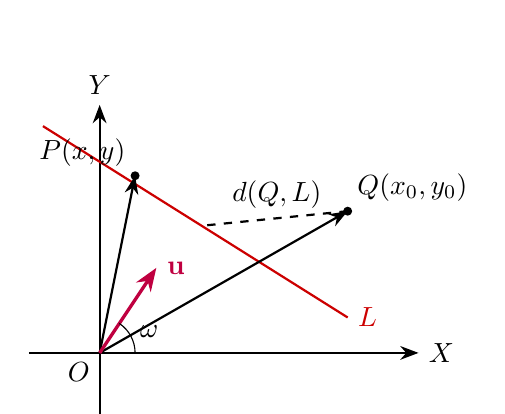
\begin{tikzpicture}[>=Stealth, scale=0.9]
  \draw[->, thick] (-1,0) -- (4.5,0) node[right] {$X$};
  \draw[->, thick] (0,-1) -- (0,3.5) node[above] {$Y$};
  \node[below left] at (0,0) {$O$};
  
  \coordinate (P) at (0.5, 2.5);
  \coordinate (Q) at (3.5, 2.0);
  \draw[thick, red!80!black] (-0.8, 3.2) -- (3.5, 0.5) node[right] {$L$};
  
  \draw[->, thick] (0,0) -- (P);
  \draw[->, thick] (0,0) -- (Q);
  \draw[dashed, thick] (Q) -- (1.5, 1.8) node[midway, above] {$d(Q,L)$};
  
  \coordinate (U) at (0.8, 1.2);
  \draw[->, very thick, purple] (0,0) -- (U) node[right] {$\mathbf{u}$};
  \draw (0.5,0) arc (0:56.3:0.5);
  \node at (0.7,0.3) {$\omega$};
  
  \fill (P) circle (1.8pt) node[above left] {$P(x,y)$};
  \fill (Q) circle (1.8pt) node[above right] {$Q(x_0,y_0)$};
\end{tikzpicture}
\caption{點到直線之垂直距離}
\label{fig:4-31}
\end{figure}

〔注意 投影量之正負依其與 $\mathbf{u}$ 同異向而定。〕
\begin{align*}
d(Q, L) &= |\vec{OQ}\cdot\mathbf{u} - \vec{OP}\cdot\mathbf{u}| \\
&= |(\cos\omega)x_0 + (\sin\omega)y_0 - p| \quad\text{〔其中 $\omega, p$ 定義已在上述 $L$ 之法線式的推導中敘明〕} \\
&= \frac{|a x_0 + b y_0 + c|}{\sqrt{a^2 + b^2}} \quad\text{〔由 (17) 式〕} \tag{26}
\end{align*}

\begin{example}[例 16]
求 $(3, 2)$ 點到直線 $2x + y = 1$ 之距離。
\end{example}

\begin{proof}[解]
所求距離 $= \frac{|2\cdot 3 + 1\cdot 2 - 1|}{\sqrt{2^2 + 1}} = \frac{7}{\sqrt{5}}$。
\end{proof}

\subsubsection*{戊、應用——等溫線；線性規劃}

設 $f(x, y) = ax + by + c$ 表平面上 $(x, y)$ 點處的溫度，\footnote{〔註〕$f(x, y)$ 為二變數 $x$ 與 $y$ 的函數，此處只討論一次函數，第四冊將介紹二次函數。}則
\[ f(x, y) = 0 \quad\text{（即 $ax + by + c = 0$）} \]
表示溫度為零度的一條等溫線 $L$。這條等溫線，可以確定地把平面隔開成溫度在零上與零下的兩個部份。道理如下：

隨便取定 $L$ 上一點 $P$，及單位法向量 $\mathbf{u}$。
設 $Q(x, y)$ 為平面上任意點，且設
\begin{align*}
g(x, y) &= \vec{OQ} \text{ 在 } \mathbf{u} \text{ 方向的投影量} - \vec{OP} \text{ 在 } \mathbf{u} \text{ 方向的投影量} \\
&= (\cos\omega)x + (\sin\omega)y - p \quad\text{〔如 (26) 式的導引〕}
\end{align*}
此值 $> 0, = 0, < 0$ 把平面由函數值 $f(x, y)$ 等於 0 的 $L$ 線隔成兩側。仔細一點討論：
\begin{enumerate}[label=(\roman*), leftmargin=2em]
  \item 當 $Q(x, y)$ 碰巧在 $L$ 上時，$g(x, y) = 0$。
  \item 當 $Q(x, y)$ 在與 $\mathbf{u}$ 的指向相反的 $L$ 的一側時，（即 $L$ 的下方，但當 $L \parallel Y$ 軸時，則為 $L$ 的左方），則有 $g(x, y) < 0$。
  \item 當 $Q(x, y)$ 在與 $\mathbf{u}$ 的指向相同的 $L$ 的一側時，則有 $g(x, y) > 0$。
\end{enumerate}

\begin{figure}[H]
\centering
\begin{tikzpicture}[>=Stealth, scale=0.85]
  \draw[->, thick] (-1,0) -- (4,0) node[right] {$X$};
  \draw[->, thick] (0,-2) -- (0,3) node[above] {$Y$};
  \node[below left] at (0,0) {$O$};
  
  \draw[thick, red!80!black] (-0.8, -1.8) -- (2.5, 3.2) node[above] {$L$};
  \coordinate (P) at (1.2, 1.2);
  \coordinate (Q) at (3.0, 1.5);
  \draw[->, very thick, purple] (P) -- ($(P) + (-0.8, 0.5)$) node[above] {$\mathbf{u}$};
  \fill (P) circle (1.8pt) node[left] {$P$};
  \fill (Q) circle (1.8pt) node[above right] {$Q(x,y)$};
  
  \node at (2.5, 2.5) {$g(x,y) > 0$};
  \node at (2.0, -1.0) {$g(x,y) < 0$};
\end{tikzpicture}
\caption{直線兩側符號分界}
\label{fig:4-32}
\end{figure}

但 $f(x, y) = 0$ 與 $g(x, y) = 0$〔後者為 $L$ 的法線式〕同樣表示 $L$，故其相應係數成比例，即存在 $k \neq 0$ 使得
\[ f(x, y) = k g(x, y) \]
故 $f > 0, f < 0$ 亦分居於 $L$ 的兩側。

要確定在 $L$ 的那一側溫度為零上，只須檢驗 $k$ 的符號。但 $\sin\omega \ge 0$，〔因有 $0 \le \omega < \pi$ 的限制〕故有：
若 $b \neq 0$，則 $b > 0 \iff k > 0$。
即當 $b > 0$ 時，$f$ 之正負按序由 $g$ 之正負決定。但 $b = 0$ 時，$\sin\omega = 0$，故 $\omega = 0, a = k\cos\omega = k$。即當 $a > 0$ 時，$k > 0$。故 $f$ 之正負按序由 $g$ 之正負決定。

\paragraph*{結論} 設 $f(x, y) \equiv ax + by + c$ 表溫度函數，則零度等溫線 $L : ax + by + c = 0$ 把平面分成零上、零下兩側：
\begin{enumerate}[label=(\roman*), leftmargin=2em]
  \item 當 $b > 0$ 時，$L$ 的上側為零上，下側為零下。
  \item 當 $b < 0$ 時，$L$ 的上側為零下，下側為零上。
  \item 當 $b = 0$ 時，零上部份居於 $L$ 之右或左按序根據 $a$ 之正或負而定。
\end{enumerate}

\begin{example}[論例 4]
繪圖判斷直線 $2x + y = 1$ 的那一側，其上的點 $(x, y)$ 滿足 $2x + y > 1$？
\end{example}

\begin{proof}[方法 1]
考慮 $f(x, y) = 2x + y - 1$，因 $y$ 之係數 $b = 1 > 0$，故上側滿足 $2x + y > 1$。
\end{proof}

\begin{proof}[方法 2]
隨便找一點 $(x_0, y_0)$ 代入 $f(x, y) = 2x + y - 1$。
若 $f(x_0, y_0) < 0$，則所求為與 $(x_0, y_0)$ 異側；
若 $f(x_0, y_0) > 0$，則所求為 $(x_0, y_0)$ 之同側。
比如取 $(x_0, y_0) = (0, 0)$，則 $f(0, 0) = -1 < 0$，故 $2x + y > 1$ 之區域在 $L$ 之上側（如圖 \ref{fig:4-33}）。
\end{proof}

\begin{figure}[H]
\centering
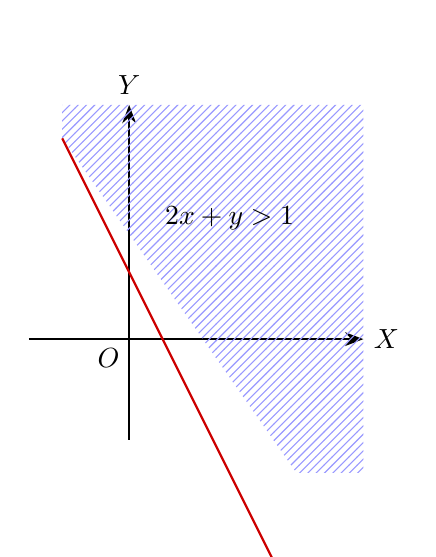
\begin{tikzpicture}[>=Stealth, scale=0.85]
  \draw[->, thick] (-1.5,0) -- (3.5,0) node[right] {$X$};
  \draw[->, thick] (0,-1.5) -- (0,3.5) node[above] {$Y$};
  \node[below left] at (0,0) {$O$};
  
  % Line: 2x + y = 1 -> y = -2x + 1
  \fill[pattern=north east lines, pattern color=blue!40] (-1, 3) -- (2.5, -2) -- (3.5, -2) -- (3.5, 3.5) -- (-1, 3.5) -- cycle;
  \draw[thick, red!80!black] (-1, 3) -- (2.2, -3.4);
  \node at (1.5, 1.8) {$2x+y>1$};
\end{tikzpicture}
\caption{半平面區域 $2x+y>1$}
\label{fig:4-33}
\end{figure}

\subsubsection*{作業 17}
繪圖判別下列直線 $f_k(x, y) = 0$ 兩側 $f_k(x, y)$ 值之正負，$k = 1, 2, 3$。
\begin{enumerate}[label=(\roman*), leftmargin=2em]
  \item $f_1(x, y) = 7x - 2y + 15 = 0$
  \item $f_2(x, y) = -3x + 6y - 1 = 0$
  \item $f_3(x, y) = -x + 2y + 1 = 0$
\end{enumerate}
這三直線把平面劃分成幾塊區域？繪圖表明每塊區域上 $f_1, f_2, f_3$ 三函數之正負。

\begin{example}[論例 5]\phantomsection\label{note:b3-ch4-p177-l1-l2-subscripts}
設 $L_1, L_2$ 為兩條相交直線：
\begin{align*}
L_1 &: f_1(x, y) = a_1 x + b_1 y + c_1 = 0\footnote{【校訂註】原書頁 177 題幹常數項均印作「$+c$」，解文中代入明確為「$+c_1$」與「$+c_2$」。正文校訂補齊下標。} \\
L_2 &: f_2(x, y) = a_2 x + b_2 y + c_2 = 0
\end{align*}
試求交角分角線方程式。
\end{example}

\begin{figure}[H]
\centering
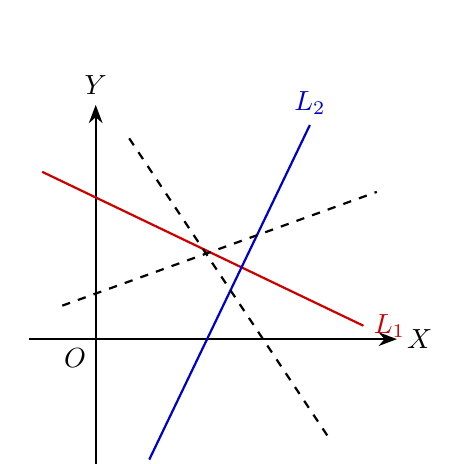
\begin{tikzpicture}[>=Stealth, scale=0.85]
  \draw[->, thick] (-1,0) -- (4.5,0) node[right] {$X$};
  \draw[->, thick] (0,-2) -- (0,3.5) node[above] {$Y$};
  \node[below left] at (0,0) {$O$};
  
  % L1, L2
  \draw[thick, red!80!black] (-0.8, 2.5) -- (4.0, 0.2) node[right] {$L_1$};
  \draw[thick, blue!80!black] (0.8, -1.8) -- (3.2, 3.2) node[above] {$L_2$};
  
  % Bisectors
  \draw[dashed, thick] (-0.5, 0.5) -- (4.2, 2.2);
  \draw[dashed, thick] (0.5, 3.0) -- (3.5, -1.5);
\end{tikzpicture}
\caption{兩直線之交角分角線}
\label{fig:4-34}
\end{figure}

\begin{proof}[解]
一點 $Q(x, y)$ 在分角線上的充要條件是
\[ d(Q, L_1) = d(Q, L_2) \]
亦即〔由 (26) 式〕
\[ \frac{|a_1 x + b_1 y + c_1|}{\sqrt{a_1^2 + b_1^2}} = \frac{|a_2 x + b_2 y + c_2|}{\sqrt{a_2^2 + b_2^2}} \]
即兩條分角線方程式分別為
\begin{equation}
\left.
\begin{aligned}
\frac{1}{\sqrt{a_1^2 + b_1^2}}(a_1 x + b_1 y + c_1) + \frac{1}{\sqrt{a_2^2 + b_2^2}}(a_2 x + b_2 y + c_2) = 0 \\
\text{與}\quad \frac{1}{\sqrt{a_1^2 + b_1^2}}(a_1 x + b_1 y + c_1) - \frac{1}{\sqrt{a_2^2 + b_2^2}}(a_2 x + b_2 y + c_2) = 0
\end{aligned}
\right\}
\label{eq:b3-4-27}
\end{equation}
\end{proof}

\subsubsection*{作業 18}
\begin{enumerate}[label=(\roman*), leftmargin=2em]
  \item 一圓切 $Y$ 軸及直線 $2x + 7y + 7 = 0$，試求其中心的軌跡方程式。
  〔提示：此中心到 $Y$ 軸與到直線 $2x + 7y - 7 = 0$ 之距離相等，利用這條件來設立方程式。〕
  \item 一動點與直線 $3x + 4y - 2 = 0$ 之距離二倍於與直線 $4x + 3y - 5 = 0$ 之距離，求其軌跡。
\end{enumerate}

如將 \eqref{eq:b3-4-27} 式重寫，可得兩條分角線方程式為：
\begin{equation}
\left(\frac{a_1}{R_1} \pm \frac{a_2}{R_2}\right)x + \left(\frac{b_1}{R_1} \pm \frac{b_2}{R_2}\right)y + \left(\frac{c_1}{R_1} \pm \frac{c_2}{R_2}\right) = 0
\label{eq:b3-4-28}
\end{equation}
其中 $R_1 = \sqrt{a_1^2 + b_1^2}, R_2 = \sqrt{a_2^2 + b_2^2}$。對 $\pm$ 號如何選定，我們作一鑑別法：

由於 $L_1$ 把平面分成 $f_1 > 0$ 及 $f_1 < 0$ 的兩側，同樣 $L_2$ 把平面分成 $f_2 > 0$ 及 $f_2 < 0$ 的兩側，因此 $L_1$ 與 $L_2$ 把平面分成四區：I、II、III、IV（見圖 \ref{fig:4-35}）。

其中在對頂的 I、III 兩區上，$f_1$ 與 $f_2$ 同號，而在另一組對頂的兩區 II、IV 上，$f_1$ 與 $f_2$ 異號。稱 I、III 兩區為 $f_1$ 與 $f_2$ 的同號區域，II、IV 兩區為 $f_1$ 與 $f_2$ 的異號區域，兩條分角線則分處於 I、III 與 II、IV。

\begin{figure}[H]
\centering
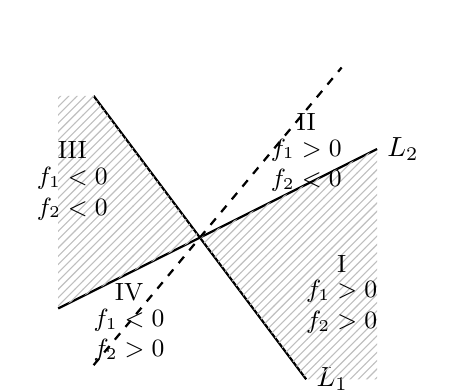
\begin{tikzpicture}[>=Stealth, scale=0.9]
  \coordinate (O) at (0,0);
  \draw[thick] (-2,-1) -- (2.5,1.25) node[right] {$L_2$};
  \draw[thick] (-1.5,2.0) -- (1.5,-2.0) node[right] {$L_1$};
  
  % Hatched regions I and III
  \fill[pattern=north east lines, pattern color=gray!50] (0,0) -- (2.5,1.25) -- (2.5,-2.0) -- (1.5,-2.0) -- cycle;
  \fill[pattern=north east lines, pattern color=gray!50] (0,0) -- (-2,-1) -- (-2,2.0) -- (-1.5,2.0) -- cycle;
  
  \node at (2.0,-0.8) {\small \shortstack{I\\$f_1>0$\\$f_2>0$}};
  \node at (1.5,1.2) {\small \shortstack{II\\$f_1>0$\\$f_2<0$}};
  \node at (-1.8,0.8) {\small \shortstack{III\\$f_1<0$\\$f_2<0$}};
  \node at (-1.0,-1.2) {\small \shortstack{IV\\$f_1<0$\\$f_2>0$}};
  
  % Dashed bisector line
  \draw[dashed, thick] (-1.5,-1.8) -- (2.0,2.4);
\end{tikzpicture}
\caption{分角線同號與異號區域}
\label{fig:4-35}
\end{figure}

\begin{proposition}
\label{prop:b3-4-2}
設 $L_1, L_2$ 兩條相交的直線的方程式分別為
\[ L_1 : f_1(x, y) = a_1 x + b_1 y + c_1 = 0, \quad L_2 : f_2(x, y) = a_2 x + b_2 y + c_2 = 0 \]
通過其交點，有兩條 $L_1$ 與 $L_2$ 的分角線分處於 $f_1$ 與 $f_2$ 之同號及異號區域，其處於同號區域之分角線方程式為：
\[ \left(\frac{a_1}{R_1} - \frac{a_2}{R_2}\right)x + \left(\frac{b_1}{R_1} - \frac{b_2}{R_2}\right)y + \left(\frac{c_1}{R_1} - \frac{c_2}{R_2}\right) = 0 \]
而處於異號區域者，方程式為：
\[ \left(\frac{a_1}{R_1} + \frac{a_2}{R_2}\right)x + \left(\frac{b_1}{R_1} + \frac{b_2}{R_2}\right)y + \left(\frac{c_1}{R_1} + \frac{c_2}{R_2}\right) = 0 \]
其中 $R_1 = \sqrt{a_1^2 + b_1^2}, R_2 = \sqrt{a_2^2 + b_2^2}$。
\end{proposition}

\begin{proof}[證明]
上面已證知分角線方程式為 \eqref{eq:b3-4-28}，今只須檢驗其正負號的判別。
在同號區域中，下二式：
\[ \frac{1}{R_1}(a_1 x + b_1 y + c_1) \quad\text{與}\quad \frac{1}{R_2}(a_2 x + b_2 y + c_2) \]
要同時大於 0 或同時小於 0，故必得兩者相減為 0，因此只有減號式是同號區域中的分角線。同理可得異號區域中為加號式。
\end{proof}

\paragraph*{註：}特殊地，當 $L_1 : f_1 = y = 0$，即 $X$ 軸；$L_2 : f_2 = x = 0$，即 $Y$ 軸時，其所分成的四區，正是平常笛卡兒座標平面上的四個象限，此時，$f_1$ 表 $y$ 座標，$f_2$ 表 $x$ 座標。

\subsubsection*{作業 19}
試求通過兩直線 $L_1 : 3x - 4y + 1 = 0$ 及 $L_2 : 4x + 3y - 1 = 0$ 交點之兩條分角線方程式，並根據 $L_1$ 與 $L_2$ 截出的四區域上面的點 $(x, y)$ 所取值 $3x - 4y + 1$ 與 $4x + 3y - 1$ 的符號，繪圖判別這兩條分角線的位置。

\begin{example}[例 17]
圖示滿足 $x + 2y - 2 < 0$ 且 $2x + y - 2 < 0$ 之 $(x, y)$ 點的範圍。
\end{example}

\begin{proof}[解]
先作 $x + 2y - 2 = 0$ 及 $2x + y - 2 = 0$ 二直線，因原點 $(0, 0)$ 滿足 $x + 2y - 2 < 0$ 及 $2x + y - 2 < 0$，故所求之區域為圖形所示斜線部份。
\end{proof}

\begin{figure}[H]
\centering
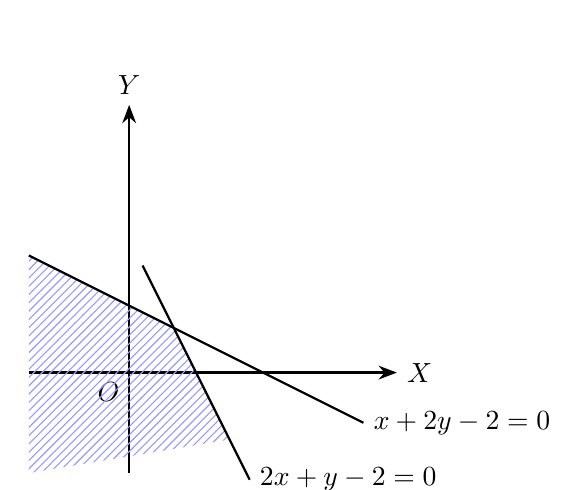
\begin{tikzpicture}[>=Stealth, scale=0.85]
  \draw[->, thick] (-1.5,0) -- (4,0) node[right] {$X$};
  \draw[->, thick] (0,-1.5) -- (0,4) node[above] {$Y$};
  \node[below left] at (0,0) {$O$};
  
  % Lines: x + 2y = 2 -> y = -0.5x + 1
  %        2x + y = 2 -> y = -2x + 2
  \coordinate (I) at (0.67, 0.67);
  \fill[pattern=north east lines, pattern color=blue!40] (-1.5, 1.75) -- (I) -- (1.5, -1) -- (-1.5, -1.5) -- cycle;
  \draw[thick] (-1.5, 1.75) -- (3.5, -0.75) node[right] {$x+2y-2=0$};
  \draw[thick] (0.2, 1.6) -- (1.8, -1.6) node[right] {$2x+y-2=0$};
\end{tikzpicture}
\caption{二元一次不等式組解區域}
\label{fig:4-36}
\end{figure}

\begin{example}[論例 6]
（線性規劃的理論基礎）
在 $x \ge 0, y \ge 0, x + 2y - 2 \le 0, 2x + y - 2 \le 0$ 之條件下，試求 $x + y$ 的最大值。
\end{example}

\begin{proof}[解]
$x \ge 0, y \ge 0, x + 2y - 2 \le 0, 2x + y - 2 \le 0$ 之區域 $D$ 如圖 \ref{fig:4-37} 所示。

則原命題即等於在區域 $D$ 內找一點 $(x, y)$，使 $x + y$ 之值為最大。令 $x + y = k$，當 $k$ 變動時，這代表一組斜率為 $-1$ 的直線，其在 $Y$ 軸上的截距為 $k$，故求 $x + y$ 的最大值即等於求 $k$ 的最大值。由圖 \ref{fig:4-37} 知當 $x = \frac{2}{3}, y = \frac{2}{3}$ 時，$x + y = \frac{4}{3}$ 為最大值。
\end{proof}

\begin{figure}[H]
\centering
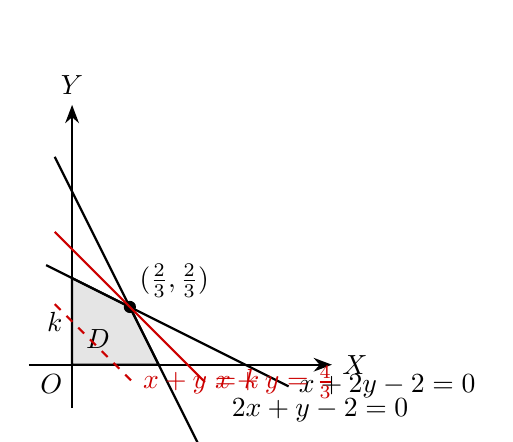
\begin{tikzpicture}[>=Stealth, scale=1.1]
  \draw[->, thick] (-0.5,0) -- (3.0,0) node[right] {$X$};
  \draw[->, thick] (0,-0.5) -- (0,3.0) node[above] {$Y$};
  \node[below left] at (0,0) {$O$};
  
  % Region D: (0,0), (1,0), (2/3, 2/3), (0,1)
  \coordinate (O) at (0,0);
  \coordinate (A) at (1,0);
  \coordinate (B) at (0.667, 0.667);
  \coordinate (C) at (0,1);
  \fill[gray!20] (O) -- (A) -- (B) -- (C) -- cycle;
  \draw[thick] (O) -- (A) -- (B) -- (C) -- cycle;
  \node at (0.3, 0.3) {$D$};
  
  % Boundary lines
  \draw[thick] (-0.3, 1.15) -- (2.5, -0.25) node[right] {$x+2y-2=0$};
  \draw[thick] (-0.2, 2.4) -- (1.5, -1.0) node[above right=10pt] {$2x+y-2=0$};
  
  \fill (B) circle (2pt) node[above right] {$(\frac{2}{3}, \frac{2}{3})$};
  
  % Objective lines
  \draw[dashed, thick, red!80!black] (-0.2, 0.7) -- (0.7, -0.2) node[right] {$x+y=k$};
  \draw[thick, red!80!black] (-0.2, 1.533) -- (1.533, -0.2) node[right] {$x+y=\frac{4}{3}$};
  \node[left] at (0, 0.5) {$k$};
\end{tikzpicture}
\caption{線性規劃目標函數最佳解}
\label{fig:4-37}
\end{figure}

\subsubsection*{作業 20}
在論例 6 之條件下，求
\begin{enumerate}[label=(\roman*), leftmargin=2em]
  \item $5x + y$ 之最大與最小值。
  \item $x + 5y$ 之最大與最小值。
  \item $x^2 + y^2$ 的最大與最小值。
  \item $xy$ 的最大與最小值。〔提示：$x + y$ 的值一定，則當 $x = y$ 時，有最大值，可比較習題 1-1 第三題。〕
\end{enumerate}

利用以上直線方程的討論，我們來考慮一堆有用的實際應用，這便是“線性規劃”的本題。

\begin{example}[論例 7]
（線性規劃）一農民有田 2 甲根據他的經驗若田地上種水稻，則每甲每期產量為 8000 斤，若種花生則每甲每期產量為 2000 斤，但水稻成本較高每甲每期需 24,000 元，花生只要 8,000 元，且花生每斤可賣 10 元，稻米只賣 6 元，現在他手頭上只能湊足 40,000 元，今假定這農民只種水稻與花生，問這農民對這兩種作物應各種地若干才能得到最大的收益？
\end{example}

\begin{proof}[解]
設水稻種 $x$ 甲，花生種 $y$ 甲，則由假設知
\[ \begin{cases}
x + y \le 2 \\
24000x + 8000y \le 40000 \\
x \ge 0, \quad y \ge 0
\end{cases}
\quad\text{或}\quad
\begin{cases}
x + y \le 2 \\
3x + y \le 5 \\
x \ge 0, \quad y \ge 0
\end{cases} \]
而利潤是
\begin{align*}
P &= (6 \times 8000 - 24000)x + (10 \times 2000 - 8000)y \\
&= 24000x + 12000y
\end{align*}
故原題意即相當於在上不等式的條件下求 $P$ 之最大值（示如圖 \ref{fig:4-38}）。

而 $24000x + 12000y = P$ 表斜率為 $-2$ 之直線，由圖知，當 $x = 1.5, y = 0.5$ 時，$P$ 有最大值 42,000（元），也就是水稻種 1.5 甲，花生種 0.5 甲最好。
\end{proof}

\begin{figure}[H]
\centering
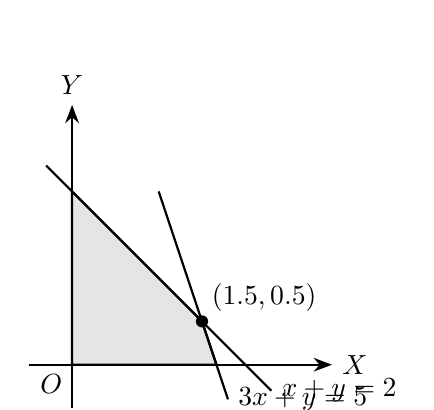
\begin{tikzpicture}[>=Stealth, scale=1.1]
  \draw[->, thick] (-0.5,0) -- (3.0,0) node[right] {$X$};
  \draw[->, thick] (0,-0.5) -- (0,3.0) node[above] {$Y$};
  \node[below left] at (0,0) {$O$};
  
  % Region: x + y <= 2, 3x + y <= 5, x >= 0, y >= 0
  % Vertices: (0,0), (5/3, 0), (1.5, 0.5), (0,2)
  \coordinate (O) at (0,0);
  \coordinate (A) at (1.667,0);
  \coordinate (B) at (1.5, 0.5);
  \coordinate (C) at (0,2);
  
  \fill[gray!20] (O) -- (A) -- (B) -- (C) -- cycle;
  \draw[thick] (O) -- (A) -- (B) -- (C) -- cycle;
  
  \draw[thick] (-0.3, 2.3) -- (2.3, -0.3) node[right] {$x+y=2$};
  \draw[thick] (1.0, 2.0) -- (1.8, -0.4) node[right] {$3x+y=5$};
  
  \fill (B) circle (2pt) node[above right] {$(1.5, 0.5)$};
\end{tikzpicture}
\caption{農作物種植利潤最大化}
\label{fig:4-38}
\end{figure}

\subsubsection*{作業 21}
\begin{enumerate}[label=(\roman*), leftmargin=2em]
  \item 假設這農民資本無限，他又應如何下種？
  \item 如果收成時市價花生上漲為每斤 12 元，稻穀下跌為每斤 5.8 元，那麼他在播種時的決定，是不是仍然是最好？
  \item 如果他另外已從農會再貸款 8000 元作為下種的資本，那麼他應該如何下種？
\end{enumerate}

\subsubsection*{習題 4-4}

\begin{enumerate}[label=\arabic*., leftmargin=2em]
  \item 求下列各直線方程式，並作其圖形。
  \begin{enumerate}[label=(\roman*), leftmargin=2em]
    \item 通過 $(1, 2)$ 而與直線 $3x - y = 6$ 平行
    \item 通過 $(-2, -3)$ 而與直線 $x + 5y - 3 = 0$ 平行
    \item 通過 $(3, -2)$ 而與直線 $2x + 3y + 4 = 0$ 垂直
    \item 通過 $(1, 5)$ 而與直線 $5x - 4y + 1 = 0$ 垂直
    \item 通過 $(2, -1)$ 而與直線 $x - y + 1 = 0$ 夾角為 $60^\circ$
  \end{enumerate}
  
  \item 求下列各對直線的夾角 $\theta$（$-\frac{\pi}{2} \le \theta \le \frac{\pi}{2}$）
  \begin{enumerate}[label=(\roman*), leftmargin=2em]
    \item $L_1 : 3x - 4y + 2 = 0, \quad L_2 : 4x + 3y - 5 = 0$
    \item $L_1 : x + 2y - 1 = 0, \quad L_2 : 2x - y + 3 = 0$
    \item $L_1 : 2x + 3y - 1 = 0, \quad L_2 : 3x - 2y + 4 = 0$
    \item $L_1 : 4x - 7y + 3 = 0, \quad L_2 : x + 2 = 0$
  \end{enumerate}
  
  \item 求下列各直線之法線式，其中 $\mathbf{u}$ 與 $\omega$ 的意義參見本節甲段，而 $\vec{OP}$ 為原點到此直線的垂線，$P$ 為垂足
  \begin{enumerate}[label=(\roman*), leftmargin=2em]
    \item $\omega = \frac{\pi}{4}, \quad \vec{OP} = 2\mathbf{u}$
    \item $\omega = \frac{2\pi}{3}, \quad \vec{OP} = -5\mathbf{u}$
    \item $\omega = \frac{5\pi}{6}, \quad \vec{OP} = \sqrt{2}\mathbf{u}$
  \end{enumerate}
  
  \item 設連接兩點 $P_1(1, 3), P_2(7, 2)$ 之線段被直線 $x - 4y + 4 = 0$ 分為兩段，求此二線段長之比。
  
  \item 化下列各直線為法線式，並求它與原點的距離及法向角。
  \begin{enumerate}[label=(\roman*), leftmargin=2em]
    \item $x + y - 1 = 0$
    \item $3x - 4y = 5$
    \item $4x - 5y = 6$
    \item $5x + 12y = 13$
  \end{enumerate}
  
  \item 求下列諸點與所給直線的距離。
  \begin{enumerate}[label=(\roman*), leftmargin=2em]
    \item $(2, 1)$ 至 $4x - 3y + 5 = 0$
    \item $(5, -3)$ 至 $x + y - 3 = 0$
    \item $(-1, -9)$ 至 $2x - 3y + 5 = 0$
    \item $(-1, 0)$ 至 $x + 2 = 0$
    \item $(7, -3)$ 至 $2y + 1 = 0$
  \end{enumerate}
  
  \item 試在 $X$ 軸上求二點，使它們到直線 $3x + 4y - 12 = 0$ 的距離為 6。
  
  \item 試求兩平行線 $3x - 4y + 5 = 0$ 與 $3x - 4y - 15 = 0$ 間之距離。
  
  \item 求通過兩直線 $3x - 4y + 1 = 0$ 及 $4x + 3y - 1 = 0$ 交點之兩條分角線方程式。
  
  \item 繪圖求滿足下列各組不等式之區域：
  \begin{enumerate}[label=(\roman*), leftmargin=2em]
    \item $2x - y - 4 > 0$
    \item $3x + y - 11 < 0$
    \item $2x - y - 4 > 0$ 且 $3x + y - 11 < 0$
    \item $2x + 3y - 6 \le 0, \quad x + y - 1 \ge 0, \quad y \ge 0$
  \end{enumerate}
  
  \item 判斷下列各點是否在所給直線之同側。
  \begin{enumerate}[label=(\roman*), leftmargin=2em]
    \item 原點與 $(3, -2)$，直線 $x - y + 1 = 0$
    \item $(1, 1), (-2, -3)$，直線 $3x - 2y - 1 = 0$
    \item $(0, 3), (-4, 0)$，直線 $2x - y + 4 = 0$
  \end{enumerate}
  
  \item 試由習題 4-2 第 7 題導出：
  \begin{align*}
  L_1 \parallel L_2 &\iff \alpha_1 = \alpha_2 \iff m_1 = m_2 \\
  L_1 \perp L_2 &\iff \alpha_1 = \alpha_2 \pm \frac{\pi}{2} \iff m_1 \cdot m_2 = -1
  \end{align*}
  
  \begin{figure}[H]
  \centering
  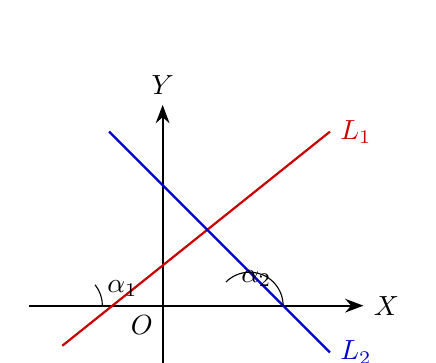
\begin{tikzpicture}[>=Stealth, scale=0.85]
    \draw[->, thick] (-2,0) -- (3,0) node[right] {$X$};
    \draw[->, thick] (0,-1) -- (0,3) node[above] {$Y$};
    \node[below left] at (0,0) {$O$};
    \draw[thick, red!80!black] (-1.5, -0.6) -- (2.5, 2.6) node[right] {$L_1$};
    \draw[thick, blue!80!black] (-0.8, 2.6) -- (2.5, -0.7) node[right] {$L_2$};
    \draw (-0.9,0) arc (0:38.6:0.5);
    \node at (-0.6, 0.25) {$\alpha_1$};
    \draw (1.8,0) arc (0:135:0.5);
    \node at (1.4, 0.4) {$\alpha_2$};
  \end{tikzpicture}
  \caption{直線傾斜角與垂直關係}
  \label{fig:4-39}
  \end{figure}
  
  \item 設某公司有兩種機器來生產某產品，第一種機器每臺要 3 萬美鈔及新臺幣 50 萬元的維護費，第二種機器每臺需美鈔 5 萬元及新臺幣 20 萬元的維護費，而第一種機器的年利潤每臺有 9 萬元，第二種的是 6 萬元的，但政府核准的外滙是美金 135 萬元，並且公司的總維護費不想超過 1,800 萬元，問每種機器應該購買幾臺最好？
  
  \item 仔細思考上題，因所買機器一定是整數，而依據代數式子解出來的最大值，如果對應點不是整數點，你該怎麼辦？
\end{enumerate}


\subsection{三線共點條件與二元一次多式聯立方程}
\label{sec:4-5}

\subsubsection*{甲、三線共點的條件}

\begin{theorem}
三直線
\begin{align*}
L_1 &= a_1 x + b_1 y + c_1 = 0 \\
L_2 &= a_2 x + b_2 y + c_2 = 0 \\
L_3 &= a_3 x + b_3 y + c_3 = 0
\end{align*}
若非相互平行（亦卽 $a_1 : a_2 : a_3 \neq b_1 : b_2 : b_3$），則其交會一點的充要條件爲
\begin{equation}
\begin{vmatrix}
a_1 & b_1 & c_1 \\
a_2 & b_2 & c_2 \\
a_3 & b_3 & c_3
\end{vmatrix} = 0
\label{eq:b3-4-29}
\end{equation}
\end{theorem}

\begin{figure}[H]
\centering
\begin{tikzpicture}[>=Stealth, scale=0.85]
  \draw[->, thick] (-1,0) -- (4.2,0) node[right] {$X$};
  \draw[->, thick] (0,-1) -- (0,4) node[above] {$Y$};
  \node[below left] at (0,0) {$O$};
  
  \coordinate (P) at (2, 2);
  \draw[thick, blue!80!black] (-0.3, 3.15) -- (3.5, 1.25) node[right] {$L_1$};
  \draw[thick, red!80!black] (-0.3, 0.85) -- (3.5, 2.75) node[above right] {$L_2$};
  \draw[thick, teal!80!black] (1.8, 3.8) -- (2.2, -0.6) node[right] {$L_3$};
  \fill (P) circle (2pt);
\end{tikzpicture}
\caption{三線共點}
\label{fig:4-40}
\end{figure}

\begin{proof}
這三線共點的問題就相當於要找一個三式聯立方程式：
\begin{equation*}
\begin{cases}
a_1 x + b_1 y + c_1 = 0 \\
a_2 x + b_2 y + c_2 = 0 \\
a_3 x + b_3 y + c_3 = 0
\end{cases}
\end{equation*}
有公解的充要條件。這裏有三個方程，才只有兩個變數 $x$ 與 $y$，要它有公解的「機會」不大，正如一般看來，平面上三條直線劃來劃去碰巧會交於一點的「機會」不大一樣。

既然假定這三線並非相互平行，則必有一對直線不相互平行。「不妨」設此不相互平行的兩直線為 $L_1, L_2$，由 \S 4-4 命題 1 知有
\[
\begin{vmatrix}
a_1 & b_1 \\
a_2 & b_2
\end{vmatrix} = a_1 b_2 - a_2 b_1 \neq 0
\]
故聯立方程式
\[
\begin{cases}
a_1 x + b_1 y + c_1 = 0 \\
a_2 x + b_2 y + c_2 = 0
\end{cases}
\]
必有唯一公解
\[
x = -\frac{\begin{vmatrix} c_1 & b_1 \\ c_2 & b_2 \end{vmatrix}}{\begin{vmatrix} a_1 & b_1 \\ a_2 & b_2 \end{vmatrix}}, \quad
y = -\frac{\begin{vmatrix} a_1 & c_1 \\ a_2 & c_2 \end{vmatrix}}{\begin{vmatrix} a_1 & b_1 \\ a_2 & b_2 \end{vmatrix}},
\]
亦卽
\begin{equation}
x = \frac{b_1 c_2 - b_2 c_1}{a_1 b_2 - a_2 b_1}, \quad y = \frac{c_1 a_2 - c_2 a_1}{a_1 b_2 - a_2 b_1}
\label{eq:b3-4-30}
\end{equation}
因此三線共點的充要條件，便是 $L_3$ 也要通過 $L_1, L_2$ 之唯一交點 \eqref{eq:b3-4-30}。

亦卽將 \eqref{eq:b3-4-30} 代入 $L_3 : a_3 x + b_3 y + c_3 = 0$ 中，所得之恒等式
\begin{equation}
a_3 \begin{vmatrix} b_1 & c_1 \\ b_2 & c_2 \end{vmatrix} - b_3 \begin{vmatrix} a_1 & c_1 \\ a_2 & c_2 \end{vmatrix} + c_3 \begin{vmatrix} a_1 & b_1 \\ a_2 & b_2 \end{vmatrix} = 0
\label{eq:b3-4-31}
\end{equation}
爲三線共點的充要條件，

但由三階行列式的定義，\eqref{eq:b3-4-31} 式剛好就是
\[
\begin{vmatrix}
a_1 & a_2 & a_3 \\
b_1 & b_2 & b_3 \\
c_1 & c_2 & c_3
\end{vmatrix} = 0 \quad \text{故得證。}
\]
\end{proof}

\noindent\textbf{註}~~定理 2 中，當三線平行時，三線會有交點的充要條件是三線疊合一道，亦卽（根據 \S 4-1，定理 1）$a_1 : a_2 : a_3 = b_1 : b_2 : b_3 = c_1 : c_2 : c_3$。

\begin{exercise}[作業 22]
問三直線 $x + y - 5 = 0, 4x + 9y + 7 = 0$ 與 $2x + 7y + 17 = 0$ 是否交會於一點？
\end{exercise}

\subsubsection*{乙、二元一次多式聯立方程}

常常我們推求一些理論尚無法處理的自然或人文的因果關係，控制因，觀察果，靠這樣實驗多次後，期望歸結出可能的因果關係。

例如有一化學作用，其過程及牽涉的分子式太過複雜，無法直接利用理論由作用諸成分的重量計算出產品的重量。於是依賴多次實驗：設做四次實驗，將甲成分 $a$ 克重、乙成分 $b$ 克重一起作用，得某主產品 $c$ 克重，其實驗數據如下：

\begin{table}[H]
\centering
\begin{tabular}{|c|c|c|c|}
\hline
\multirow{2}{*}{實~~驗} & \multicolumn{2}{c|}{因} & 果 \\
\cline{2-4}
 & 甲成分重 $a$ & 乙成分重 $b$ & 主產品重 $c$ \\
\hline
第 1 次 & 2 & 3 & 1 \\
第 2 次 & 1 & 4 & 1 \\
第 3 次 & 3 & 4 & 2 \\
第 4 次 & 3 & 2 & 1 \\
\hline
\end{tabular}
\end{table}

初步，我們希望有一個一次關係式\footnote{注意主產品的重 $c$ 爲各成分之重 $a, b$ 的函數，其實際關係式可能相當複雜，初步所設的一次關係式爲最粗略的估計，第四冊將介紹二次式做估計。}
\[
c = ax + by
\]
並求出來 $x$ 與 $y$，而使每一次實驗數據 $a, b, c$ 均滿足這一關係式。假如這個眞辦得到，我們便可用它來推測未做實驗的結果，更可用來計劃這產品的製造過程。

換句話說，我們初步的希望是：下面聯立方程式中的 $x, y$ 可解：
\begin{equation}
\begin{cases}
2x + 3y = 1 \\
x + 4y = 1 \\
3x + 4y = 2 \\
3x + 2y = 1
\end{cases}
\label{eq:b3-4-32}
\end{equation}
但是一般說來這待定變數（$x$ 與 $y$）只有兩個，而方程式卻有四個，這樣的聯立方程組可有解的「機會」太小了。

把這問題轉化成幾何，便是 \eqref{eq:b3-4-32} 中四個式子所代表的四條直線何時交會於一點的問題，四條直線要交會於一點的「機會」\footnote{這裡所謂「機會」可以這樣了解：作一輪盤及一射針，急劇轉動輪盤，將此針插射其上，每插射兩次，得兩點連結起來一直線，一個實驗射八次，得四直線，多做幾十次實驗，會發覺四直線共點的機會幾近於 0，另一方面，若每實驗僅射四次得兩直線，它們會平行或重疊的機會也幾近於 0，顯示二元一次二式聯立方程絕大部份的時候有唯一解。}太小了。如果僥倖四直線共點，亦卽 \eqref{eq:b3-4-32} 式有解，則我們便已求得所要的關係式。如果無解，則可利用「最小二乘方法」來求它的一個逼近的解。

\begin{figure}[H]
\centering
\begin{tikzpicture}[>=Stealth, scale=0.9]
  \draw[thick] (0,0) ellipse (1.6cm and 0.65cm);
  \draw[double, thick] (0,0) -- (0,-1.3);
  \draw[->, thick] (-1.3, 0.38) arc (160:200:1.6cm and 0.65cm);
  \draw[->, thick] (1.3, -0.38) arc (-20:20:1.6cm and 0.65cm);
  % pointer / needle
  \draw[thick] (1.05, 1.4) -- (0.8, 0.3);
  \draw[thick] (1.0, 1.45) -- (1.15, 1.35) -- (1.25, 1.55) -- (1.1, 1.65) -- cycle;
  % needle stuck in wheel
  \draw[thick] (0.35, 0.45) -- (0.35, 0.1);
  \fill (0.35, 0.1) circle (1.5pt);
\end{tikzpicture}
\caption{轉盤與射針}
\label{fig:4-41}
\end{figure}

\noindent\textbf{注意：}如果所解得的關係式中 $x > y$，則表示甲成分影響產品的效力大。適當地調整實驗中的 $a, b$，可由其實驗結果看出某成分是否只為催化劑還是真正參與化學作用。

將 \eqref{eq:b3-4-32} 式的求解一般化起來，便成爲如下的二元一次多式聯立方程
\begin{equation}
\begin{cases}
a_1 x + b_1 y + c_1 = 0 \\
a_2 x + b_2 y + c_2 = 0 \\
\quad \vdots \\
a_n x + b_n y + c_n = 0
\end{cases} \quad (\text{共有 } n \text{ 式})
\label{eq:b3-4-33}
\end{equation}
要處理這問題，先假設 \eqref{eq:b3-4-33} 中各式所代表的直線不是都相互平行。〔因如都相互平行，則 \eqref{eq:b3-4-33} 式有解的充要條件是各式所代表的直線全部重疊在一起，亦卽各式的係數全部相應成比例，卽：
\[
a_1 : b_1 : c_1 = a_2 : b_2 : c_2 = \cdots = a_n : b_n : c_n
\]
此時 \eqref{eq:b3-4-33} 式的解是 $a_1 x + b_1 y + c_1 = 0$ 所代表的整條直線，是否這樣，很容易檢驗出來。〕

\begin{theorem}
一般的二元一次多式聯立方程
\begin{equation}
\begin{cases}
a_1 x + b_1 y + c_1 = 0 \\
a_2 x + b_2 y + c_2 = 0 \\
\quad \vdots \\
a_n x + b_n y + c_n = 0
\end{cases}
\label{eq:b3-4-34}
\end{equation}
若各式所代表的直線並非完全相互平行，則可取其中相交的兩直線，比如說所取的是
\begin{align*}
L_1 &: a_1 x + b_1 y + c_1 = 0 \\
L_2 &: a_2 x + b_2 y + c_2 = 0
\end{align*}
兩式所代表的直線（$a_1 : b_1 \neq a_2 : b_2$）。此時這聯立方程有唯一解的充要條件是對於所有的 $i = 3, 4, \dots, n$
\begin{equation}
\begin{vmatrix}
a_1 & b_1 & c_1 \\
a_2 & b_2 & c_2 \\
a_i & b_i & c_i
\end{vmatrix} = 0
\label{eq:b3-4-35}
\end{equation}
\end{theorem}

\begin{proof}
從甲段三線共點的條件，可看出本定理只是直接的應用。既然 $L_1, L_2$ 相交於一點 $A$，則整個聯立方程式要有解的充要條件是其他任何式子所代表的直線
\[
L_i : a_i x + b_i y + c_i = 0
\]
都要通過這 $L_1$ 與 $L_2$ 的交點 $A$，換句話說，對任何 $i = 3, 4, \dots, n$，$L_1, L_2, L_i$ 必須共點，亦卽
\[
\begin{vmatrix}
a_1 & b_1 & c_1 \\
a_2 & b_2 & c_2 \\
a_i & b_i & c_i
\end{vmatrix} = 0
\]
\end{proof}

\begin{figure}[H]
\centering
\begin{minipage}[b]{0.46\textwidth}
\centering
\begin{tikzpicture}[>=Stealth, scale=0.85]
  \coordinate (A) at (0, 0);
  \draw[thick] (-2, -0.4) -- (2, 0.4) node[right] {$L_1$};
  \draw[thick] (-1.2, -1.8) -- (1.2, 1.8) node[above] {$L_4$};
  \draw[thick] (-1.8, -1.2) -- (1.8, 1.2) node[below right] {$L_2$};
  \draw[thick] (-1.2, 1.5) -- (1.2, -1.5) node[right] {$L_3$};
  \fill (A) circle (1.5pt) node[below right=2pt] {$A$};
\end{tikzpicture}
\caption{有唯一解 $A$}
\label{fig:4-42}
\end{minipage}
\hfill
\begin{minipage}[b]{0.46\textwidth}
\centering
\begin{tikzpicture}[>=Stealth, scale=0.85]
  \coordinate (A) at (0, 0.5);
  \draw[thick] (-2, -0.5) -- (2, 1.5) node[right] {$L_1$};
  \draw[thick] (-1.5, 1.5) -- (1.5, -0.5) node[below left] {$L_2$};
  \draw[thick] (-0.8, -1.5) -- (1.8, 1.2) node[below right] {$L_4$};
  \draw[thick] (-0.3, 1.8) -- (0.8, -1.8) node[right] {$L_3$};
  \fill (A) circle (1.5pt) node[below=2pt] {$A$};
\end{tikzpicture}
\caption{無解}
\label{fig:4-43}
\end{minipage}
\end{figure}

\subsubsection*{習題 4-5}
\begin{enumerate}
\item 問下列聯立方程是否有解，有則解之；並畫出其相應的幾何圖形（卽各直線的相關位置）。
  \begin{enumerate}[(i)]
    \item $\begin{cases} 2x + 3y = 1 \\ 6x + 9y - 3 = 0 \\ 4x + 6y = 2 \end{cases}$
    \item $\begin{cases} 2x + 3y = 1 \\ 6x + 9y - 3 = 0 \\ 4x + 6y = 1 \end{cases}$
    \item $\begin{cases} 2x + 3y = 1 \\ 6x + 9y - 3 = 0 \\ x + y = 2 \end{cases}$
    \item $\begin{cases} 2x + 3y = 1 \\ 6x + 9y - 3 = 0 \\ x + y = 2 \\ 4x + 6y = 1 \end{cases}$
  \end{enumerate}

\item 下列聯立方程是否有解？
  \begin{enumerate}[(i)]
    \item $\begin{cases} 2x + 3y = 1 \\ x + y = 2 \\ 5x + 6y = 7 \\ x + 2y + 1 = 0 \end{cases}$
    \item $\begin{cases} 2x + 3y = 1 \\ x + y = 2 \\ x + 2y + 1 = 0 \\ 2x - y = 3 \end{cases}$
  \end{enumerate}
\end{enumerate}

\subsection{* 直線系與自由度}
\label{sec:4-6}

\subsubsection*{甲、共點直線系}

平面上所有通過一定點 $A_0(x_0, y_0)$ 的直線全體組成一個集合，稱爲一個共點直線系。但很多時候，我們已知其中相交兩直線 $L_1, L_2$ 的方程式，若可不求出 $L_1$ 與 $L_2$ 交點 $A_0$ 的座標 $x_0, y_0$ 而能寫出這共點直線系的一般方程式，則很能簡化問題的處理。

\begin{figure}[H]
\centering
\begin{tikzpicture}[>=Stealth, scale=0.9]
  \coordinate (A) at (1.5, 2.5);
  \coordinate (B) at (0, 0);
  \coordinate (C) at (3.5, 0);
  \coordinate (M) at (1.75, 0);
  
  \draw[thick] (A) -- (B) -- (C) -- cycle;
  \draw[thick] (A) -- (M);
  \node[above] at (A) {$A$};
  \node[left] at (B) {$B$};
  \node[right] at (C) {$C$};
  \node[below] at (M) {$M$};
\end{tikzpicture}
\caption{三角形中線}
\label{fig:4-44}
\end{figure}

比如說，已知一三角形兩邊 $AB, AC$ 的直線方程，要求第三邊 $BC$ 的中線，我們不須求出 $A$ 的座標，先寫下通過 $A$ 的一般方程式，其中的參數再由中線要通過底邊 $BC$ 的中點 $M$ 這一特徵來決定。

\begin{theorem}
已知相交兩直線
\begin{align*}
L_1 &: a_1 x + b_1 y + c_1 = 0 \\
L_2 &: a_2 x + b_2 y + c_2 = 0
\end{align*}
則直線 $L$ 會通過 $L_1$ 與 $L_2$ 交點的充要條件是 $L$ 可以寫成
\begin{equation}
\alpha(a_1 x + b_1 y + c_1) + \beta(a_2 x + b_2 y + c_2) = 0
\label{eq:b3-4-36}
\end{equation}
其中 $\alpha, \beta$ 爲某兩實數。
\end{theorem}

\begin{proof}
若 $L$ 可寫成 \eqref{eq:b3-4-36} 式\footnote{\phantomsection\label{note:b3-ch4-p193-formula-ref}【校訂註】原書頁 193 證明首行印作「若 $L$ 可寫成(1)式」，依上下文校訂指上一頁式 \eqref{eq:b3-4-36}。}，則必然通過 $L_1, L_2$ 交點 $A_0(x_0, y_0)$。道理是因為 $a_1 x_0 + b_1 y_0 + c_1 = 0$ 且 $a_2 x_0 + b_2 y_0 + c_2 = 0$，
故
\[
\alpha(a_1 x_0 + b_1 y_0 + c_1) + \beta(a_2 x_0 + b_2 y_0 + c_2) = 0
\]
反過來，若一直線
\[
L : ax + by + c = 0 \quad [a \text{ 與 } b \text{ 不全爲 } 0]
\]
通過 $L_1$ 與 $L_2$ 交點，則因 $L_1, L_2$ 相交，$\begin{vmatrix} a_1 & b_1 \\ a_2 & b_2 \end{vmatrix} \neq 0$。

故可以解出下列聯立方程式
\[
\begin{cases}
a_1 \alpha + a_2 \beta = a \\
b_1 \alpha + b_2 \beta = b
\end{cases}
\]
中之 $\alpha$ 與 $\beta$。因此 $L$ 之方程式可寫成：
\begin{equation}
L : \alpha(a_1 x + b_1 y) + \beta(a_2 x + b_2 y) + c = 0
\label{eq:b3-4-37}
\end{equation}
今 $L$ 依假設通過 $A_0(x_0, y_0)$ 點，故 $(x_0, y_0)$ 滿足 \eqref{eq:b3-4-37} 式，得
\[
\alpha(a_1 x_0 + b_1 y_0) + \beta(a_2 x_0 + b_2 y_0) + c = 0
\]
或
\[
\alpha c_1 + \beta c_2 = c
\]
故代回 \eqref{eq:b3-4-37} 式，得：
\[
L : \alpha(a_1 x + b_1 y + c_1) + \beta(a_2 x + b_2 y + c_2) = 0. \qedhere
\]
\end{proof}

上述定理顯示通過 $L_1$ 與 $L_2$ 交點 $A_0$ 之共點直線系爲
\[
\{\alpha(a_1 x + b_1 y + c_1) + \beta(a_2 x + b_2 y + c_2) = 0 \mid \alpha, \beta \in \mathbb{R},\ \alpha, \beta \text{ 不同時爲 } 0\}。
\]
其實對 $\alpha : \beta$ 的比例一樣的所有 $\alpha, \beta$
\begin{equation}
\alpha(a_1 x + b_1 y + c_1) + \beta(a_2 x + b_2 y + c_2) = 0
\label{eq:b3-4-38}
\end{equation}
都代表同一直線，故只要 \eqref{eq:b3-4-38} 式不正好看作代表 $L_2$，則 $\alpha \neq 0$ 可將 \eqref{eq:b3-4-38} 式兩端除以 $\alpha$，得
\[
(a_1 x + b_1 y + c_1) + k(a_2 x + b_2 y + c_2) = 0
\]
其中 $k = \frac{\beta}{\alpha}$。因此參數減少成為只有 $k$ 一個。我們得：

\begin{theorem}
已知相交兩直線
\begin{align*}
L_1 &: a_1 x + b_1 y + c_1 = 0 \\
L_2 &: a_2 x + b_2 y + c_2 = 0
\end{align*}
則直線 $L$ 不是 $L_2$ 本身，又要通過 $L_1$ 與 $L_2$ 交點的充要條件是 $L$ 可以寫成
\[
L : (a_1 x + b_1 y + c_1) + k(a_2 x + b_2 y + c_2) = 0
\]
其中 $k$ 爲某一實數。
\end{theorem}

這定理其實比前面定理在計算時有用，因只牽涉到一個參數，這樣只要再加上一個條件就能決定 $L$ 的確實位置及其方程表示了。

\begin{example}
設
\begin{align*}
L_1 &: 2x - y = 2 \\
L_2 &: x + 3y = 5 \\
L_3 &: y = 0
\end{align*}
三條直線圍成一個三角形 $\triangle ABC$，求 $L_3$ 邊上的中線方程式。
\end{example}

\begin{figure}[H]
\centering
\begin{tikzpicture}[>=Stealth, scale=0.9]
  \coordinate (B) at (1, 0);
  \coordinate (C) at (5, 0);
  \coordinate (A) at (1.57, 1.14);
  \coordinate (M) at (3, 0);
  
  \draw[thick] (0, 0) -- (6, 0);
  \draw[thick] (0.8, -0.4) -- (2.2, 2.4) node[above] {$L_1$};
  \draw[thick] (5.8, -0.27) -- (0.8, 1.4) node[above] {$L_2$};
  \draw[thick, blue!80!black] (1.3, 1.36) -- (3.7, -0.56) node[below] {$L$};
  
  \fill (B) circle (1.5pt) node[below] {$B(1, 0)$};
  \fill (C) circle (1.5pt) node[below] {$C(5, 0)$};
  \fill (M) circle (1.5pt) node[below] {$M$};
  \fill (A) circle (1.5pt) node[right=2pt] {$A$};
\end{tikzpicture}
\caption{求三角形中線}
\label{fig:4-45}
\end{figure}

\begin{proof}[解]
設所求中線爲 $L$，則 $L$ 可寫成
\begin{equation}
L : (2x - y - 2) + k(x + 3y - 5) = 0
\label{eq:b3-4-39}
\end{equation}
其中 $k$ 爲待定實數，應依 $L$ 通過 $BC$ 中點 $M$ 決定。

今 $B$ 爲 $L_1, L_3$ 交點易知爲 $(1, 0)$，\\
$C$ 爲 $L_2, L_3$ 交點易知爲 $(5, 0)$，\\
故 $M = (3, 0)$。

因 $M$ 在 $L$ 上，故代 $(3, 0)$ 入 \eqref{eq:b3-4-39} 式，應滿足 \eqref{eq:b3-4-39} 式，由此決定出 $k$：
\[
(6 - 2) + k(3 - 5) = 0
\]
因此 $k = 2$ 代回 \eqref{eq:b3-4-39} 式，得中線 $L$ 的方程式爲
\[
L : 4x + 5y - 12 = 0. \qedhere
\]
\end{proof}

\begin{exercise}[作業 23]
利用本段方法，寫出
\begin{align*}
L_1 &: 2x - y = 2 \\
L_2 &: x + 3y = 5 \\
L_3 &: x + y + 1 = 0
\end{align*}
三直線所圍成 $\triangle ABC$ 之三個高之方程式，然後利用 \S 4-5 中三線共點之行列式條件證明這三個高共點。
\end{exercise}

\begin{exercise}[**作業 24]
利用本定理 4 的觀念證明行列式中一件要緊事實：
\[
\text{一個行列式 } A : \begin{vmatrix} a_1 & b_1 & c_1 \\ a_2 & b_2 & c_2 \\ a_3 & b_3 & c_3 \end{vmatrix} = 0 \iff \text{經過行列式基本運算，$A$ 能變成一新行列式，其中有一列全爲 0。}
\]
\end{exercise}

\begin{exercise}[**作業 25]
利用 \S 4-5 所論三線共點的行列式條件及作業 24 所述事實，來說明本段共點直線系的主要定理。
\end{exercise}

\noindent\textbf{習題}~~試作附錄二中「聯立方程式求解的幾何解釋」之題組測驗。

\subsubsection*{* 乙、自由度}

我們生活的空間常特稱爲三度空間，這裏所稱的三度是三個自由度的意思。換句話說，一個點在三度空間中運動，它有前後、左右、上下可以伸展（如空中鳥的飛行）。至於限制在一給定平面上運動的物體，只有前後、左右可以伸展（如在平面上溜冰）。而限制在一給定直線上運動的物體，更只有前後可以伸展（如火車在鐵軌上行駛）。我們說平面（作爲其上點的集合來看）的自由度是 2。有時把平面稱爲二度空間。直線（作爲其上點的集合來看）的自由度是 1，有時把直線稱爲一度空間。

先注意一件事：利用座標，空間中的點，可由三個實數來準確地描寫。同樣，平面與直線上的點，也可分別由兩個或一個實數來描寫。

\begin{figure}[H]
\centering
\begin{tikzpicture}[>=Stealth, scale=0.95]
  \draw[->, thick] (0,0) -- (3.5,0) node[right] {$Y$};
  \draw[->, thick] (0,0) -- (0,3) node[above] {$Z$};
  \draw[->, thick] (0,0) -- (-2,-1.5) node[below left] {$X$};
  \node[above left] at (0,0) {$O$};
  
  \coordinate (Px) at (-1.2, -0.9);
  \coordinate (Pxy) at (1.3, -0.9);
  \coordinate (P) at (1.3, 0.9);
  
  \draw[thick, dashed] (0,0) -- (Px) -- (Pxy) -- (P);
  \draw[thick] (0,0) -- (P);
  \fill (P) circle (1.5pt);
  
  \draw[|<->|] (-1.4, -0.7) -- (-0.2, 0.2) node[midway, above left, sloped] {$x$ 單位};
  \draw[|<->|] (-1.2, -1.2) -- (1.3, -1.2) node[midway, below] {$y$ 單位};
  \draw[|<->|] (1.6, -0.9) -- (1.6, 0.9) node[midway, right] {$z$ 單位};
\end{tikzpicture}
\caption{空間直角座標系}
\label{fig:4-46}
\end{figure}

例如，取空間一個直角座標系 $(O; X, Y, Z)$，空間每一點可以用它相應的座標 $(x, y, z)$ 來表示。換句話說，將一個點一開始座標的位置取爲原點 $O$，則它可能伸展的運動範圍可由它運動後的新位置來描寫，而這些新位置又可由該點從 $O$ 前後移動 $x$ 單位，左右移動 $y$ 單位，然後再加上下移動 $z$ 單位來決定，也就是說：空間中點可能伸展的運動範圍可用三個實數 $x, y, z$ 來描寫，這些實數的個數 3，便是這空間裏點的自由度。

我們把這種用自由度來表示點可能伸展的運動範圍的觀點應用到較一般的集合上：

\begin{example}
平面上所有以原點 $O$ 爲心的同心圓，這樣的集合 $S_1$，稱爲一個同心圓系，裏頭每一個元素是一個以 $O$ 爲心的圓，我們可以經由指定它們的半徑長 $k$ 來準確挑出這圓系中的一個圓（如果考慮的集合不是 $S_1$ 而是平面上圓的全體，則給了半徑長，卻有無數個圓的半徑正好是這一長度）。例如圖 \ref{fig:4-47} 中，$k = 3$ 表示半徑爲 3 的圓 $C_3 : x^2 + y^2 = 3^2$，$k = \frac{1}{2}$ 表示半徑爲 $\frac{1}{2}$ 的圓 $C_{\frac{1}{2}} : x^2 + y^2 = \left(\frac{1}{2}\right)^2$。換句話說：利用一個非負的實數 $k$，我們對應地描寫出這集合 $S_1$ 中的元素。因爲所用的實數正好是一個，我們稱這集合 $S_1$ 的自由度爲 1。
\[
S_1 = \{x^2 + y^2 = k^2 \mid k \in \mathbb{R}\}
\]
傳統上，我們常稱這個實數 $k$，爲圓系 $S_1$ 的一個參數。
\end{example}

\begin{exercise}[作業 26]
平面上所有的圓自由度若干？指出它相應的參數。注意取正交座標系，平面上圓的一般方程式爲 $(x - a)^2 + (y - b)^2 = k^2$。
\end{exercise}

\begin{example}
一個曲面上點的集合同平面上點的集合一樣，自由度爲 2，例如地球表面任給一點可沿經度、緯度作南北、東西的運動（南北極除外），這時經度、緯度就是它的兩個參數。如果恰巧所給的點是兩極之一，仍可另創一系經緯來描寫極點附近的運動，自由度仍爲 2。
\end{example}

\begin{figure}[H]
\centering
\begin{tikzpicture}[>=Stealth, scale=0.85]
  \draw[->, thick] (-2.8,0) -- (2.8,0);
  \draw[->, thick] (0,-2.8) -- (0,2.8);
  \draw (0,0) circle (0.4);
  \draw (0,0) circle (0.8);
  \draw (0,0) circle (1.3);
  \draw (0,0) circle (2.2);
  \node[above right] at (1.55, 1.55) {$C_3$};
\end{tikzpicture}
\caption{同心圓系}
\label{fig:4-47}
\end{figure}

\begin{example}
設 $S_2$ 表示平面上所有直線構成的集合，它的自由度爲 2。想法是取一座標系 $(O; X, Y)$，則根據法線式，每一直線可由它的傾斜程度（由法向量之矢角 $\omega$ 決定）及它到原點 $O$ 的距離 $p$（可正可負）決定：
\[
(\cos\omega)x + (\sin\omega)y = p
\]
此時 $\omega$ 與 $p$ 便是相應的兩個參數，故 $S_2$ 自由度爲 2，也就是說 $S_2$ 中直線既可轉動，又可平行移動，卽 $S_2$ 有它的自由度。

今固定 $\omega$，則得一平行直線系 $S_2'$，例如，取 $\omega = \frac{2\pi}{3}$，則
\[
\cos\frac{2\pi}{3} = -\frac{1}{2}, \quad \sin\frac{2\pi}{3} = \frac{\sqrt{3}}{2}
\]
\[
S_2' = \left\{ -\frac{x}{2} + \frac{\sqrt{3}y}{2} = p \;\middle|\; p \in \mathbb{R} \right\}
\]
$p$ 爲 $S_2'$ 之唯一參數，亦卽 $S_2'$ 之自由度爲 1。
\end{example}

\begin{figure}[H]
\centering
\begin{minipage}[b]{0.46\textwidth}
\centering
\begin{tikzpicture}[>=Stealth, scale=0.85]
  \draw[->, thick] (-2,0) -- (2.5,0) node[right] {$X$};
  \draw[->, thick] (0,-1.5) -- (0,2.5) node[above] {$Y$};
  \node[below left] at (0,0) {$O$};
  
  \draw[->, thick] (0,0) -- (-0.6, 1.04) node[midway, left] {$p$};
  \draw (0.5,0) arc (0:120:0.5);
  \node at (0.35, 0.45) {$\omega$};
  
  \draw[thick, blue!80!black] (-1.8, 0.35) -- (0.6, 1.73);
  \draw (-0.5, 0.87) -- (-0.33, 0.97) -- (-0.43, 1.14);
\end{tikzpicture}
\caption{法線式參數}
\label{fig:4-48}
\end{minipage}
\hfill
\begin{minipage}[b]{0.46\textwidth}
\centering
\begin{tikzpicture}[>=Stealth, scale=0.85]
  \draw[->, thick] (-2,0) -- (2.5,0);
  \draw[->, thick] (0,-2) -- (0,2.5);
  
  \draw[->, thick] (0,0) -- (-1.2, 2.08);
  \draw (0.5,0) arc (0:120:0.5);
  \node at (0.4, 0.5) {$\frac{2\pi}{3}$};
  
  \foreach \c in {-1.5, -1.0, -0.5, 0, 0.5, 1.0, 1.5, 2.0} {
    \draw[thick, teal!80!black] (-2, {-2*0.577 + \c}) -- (2, {2*0.577 + \c});
  }
  \node[below] at (0, -1.2) {$S_2'$};
\end{tikzpicture}
\caption{平行直線系 $S_2'$}
\label{fig:4-49}
\end{minipage}
\end{figure}

\begin{exercise}[作業 27]
設通過 $(0, 3)$ 點的所有直線的集合爲 $S$，求 $S$ 的自由度及其相應參數。
\end{exercise}

\begin{exercise}[作業 28]
球面上所謂大圓，便是球面與通過球心的平面的交線〔小圓則爲球面與任一平面（不須通過球心）的交線〕。問球面上所有大圓的集合自由度若干？
\end{exercise}

\begin{figure}[H]
\centering
\begin{tikzpicture}[>=Stealth, scale=0.9]
  \draw[thick] (0,0) circle (1.5);
  \draw[thick, dashed] (1.5,0) arc (0:180:1.5cm and 0.45cm);
  \draw[thick] (-1.5,0) arc (180:360:1.5cm and 0.45cm);
  \fill (0,0) circle (1.5pt) node[below left] {$O$};
  
  \draw[thick] (-2, -0.6) -- (1.2, -0.6) -- (2, 0.6) -- (-1.2, 0.6) -- cycle;
  \draw[thick, blue!80!black] (0,0) ellipse (1.5cm and 0.45cm);
\end{tikzpicture}
\caption{球面大圓}
\label{fig:4-50}
\end{figure}

\begin{exercise}[作業 29]
一個物體 $M$，取定其中一點 $O$，設 $S$ 爲所有以 $O$ 爲固定點的轉動，卽 $S$ 中每一元素本身便是物體 $M$，以 $O$ 爲心的一個轉動，如：圖 \ref{fig:4-51}, \ref{fig:4-52}。問 $S$ 的自由度若干？
\end{exercise}

\begin{figure}[H]
\centering
\begin{minipage}[b]{0.56\textwidth}
\centering
\begin{tikzpicture}[>=Stealth, scale=0.85]
  \draw[thick] plot [smooth cycle, tension=0.8] coordinates {(-2.5, 0) (-2.8, 1) (-2.2, 1.8) (-1.8, 1.2) (-1.5, 0.5) (-1.8, -0.5) (-2.2, -0.8)};
  \fill (-2.0, 0.3) circle (1.5pt) node[below] {$O$};
  \draw[dashed] (-2.0, 0.3) ellipse (0.4cm and 0.15cm);
  
  \draw[->, thick] (-1.0, 0.5) -- (-0.2, 0.5) node[midway, above] {轉成};
  
  \draw[thick] plot [smooth cycle, tension=0.8] coordinates {(0.8, -0.5) (1.2, -0.8) (1.8, 0) (2.5, 0.8) (2.0, 1.8) (1.2, 1.2) (0.5, 0.5)};
  \fill (1.3, 0.5) circle (1.5pt) node[below left] {$O$};
  \draw[dashed] (1.3, 0.5) ellipse (0.3cm and 0.4cm);
\end{tikzpicture}
\caption{剛體以 $O$ 爲固定點之轉動}
\label{fig:4-51}
\end{minipage}
\hfill
\begin{minipage}[b]{0.36\textwidth}
\centering
\begin{tikzpicture}[>=Stealth, scale=0.85]
  \draw[thick] (0,0) circle (1.2);
  \draw[thick, dashed] (1.2,0) arc (0:180:1.2cm and 0.35cm);
  \draw[thick] (-1.2,0) arc (180:360:1.2cm and 0.35cm);
  \fill (0,0) circle (1.5pt) node[below right] {$O$};
\end{tikzpicture}
\caption{球面以 $O$ 爲固定點}
\label{fig:4-52}
\end{minipage}
\end{figure}

\begin{exercise}[作業 30]
空間中所有直線的自由度爲若干？
\end{exercise}


\subsection{\texorpdfstring{$\ddagger$ }{‡ }座標幾何與向量幾何混合處理的典型與例子（三角形諸心問題）}
\label{sec:4-7}

\subsubsection*{甲、重心的物理意義}

在平面幾何中，我們採用以全等三角形定理爲核心發展出來的技巧，證明過所謂三角形諸心定理（重心、垂心、外心、內心、傍心）。以下我們要用向量與座標幾何來處理這些問題。這處理過程的計算稍嫌複雜，但它有一定的脈絡，這是系統處理與非系統處理的主要分別。

我們先舉重心這一較富物理意義的例子來解釋這一問題的本質。

拿起一塊密度均勻的三角板，以其一頂點當支點懸空提起，則通過該頂點的鉛垂線，必因其兩側「力矩」平衡，而須通過底邊中點，亦卽如圖 \ref{fig:4-53} $\overline{BM} = \overline{MC}$。

\begin{figure}[H]
\centering
\begin{tikzpicture}[>=Stealth, scale=0.9]
  \coordinate (A) at (1, 2.5);
  \coordinate (B) at (-0.6, 0.6);
  \coordinate (C) at (2.6, -0.6);
  \coordinate (M) at (1, 0);
  
  \foreach \x in {-0.4, -0.1, 0.2, 0.5, 0.8, 1.2, 1.5, 1.8, 2.1, 2.4} {
    \draw[gray!50, thin] (\x, {2.5 - (2.5 - (\x < 1 ? 0.6 : -0.6))*abs(\x - 1)/1.6}) -- (\x, {0.6 - 1.2*(\x + 0.6)/3.2});
  }
  
  \draw[thick] (A) -- (B) -- (C) -- cycle;
  \draw[thick, dashed] (A) -- (M);
  
  \node[above] at (A) {$A$};
  \node[left] at (B) {$B$};
  \node[right] at (C) {$C$};
  \node[below left] at (M) {$M$};
  
  \draw[thick] (0.8, 2.7) -- (1.2, 2.7);
  \draw[thick] (1, 2.7) -- (1, 2.5);
\end{tikzpicture}
\caption{懸空提起三角板}
\label{fig:4-53}
\end{figure}

這聯結一頂點與對邊中點的直線稱爲三角形的一條中線。

仔細地對三個頂點都做同樣的實驗，我們發覺所得三條中線幾乎都交於一點。這一點，在物理上有它的代表意義。我們稱之爲重心。

我們能否在數學上證明任意三角形三中線都要交於一點，來表示我們上述實驗的推論其實對所有形狀的三角形都是正確的。

\begin{figure}[H]
\centering
\begin{tikzpicture}[>=Stealth, scale=0.9]
  \coordinate (A) at (1.5, 2.8);
  \coordinate (B) at (0, 0);
  \coordinate (C) at (4, 0);
  \coordinate (M) at (2, 0);
  \coordinate (N) at ($(A)!0.5!(C)$);
  \coordinate (R) at ($(A)!0.5!(B)$);
  \coordinate (G) at (barycentric cs:A=1,B=1,C=1);
  
  \draw[thick] (A) -- (B) -- (C) -- cycle;
  \draw[thick, blue!80!black] (A) -- (M);
  \draw[thick, blue!80!black] (B) -- (N);
  \draw[thick, blue!80!black] (C) -- (R);
  
  \fill (G) circle (1.5pt) node[below=2pt] {$G$};
  \node[above] at (A) {$A$};
  \node[left] at (B) {$B$};
  \node[right] at (C) {$C$};
  \node[below] at (M) {$M$};
  \node[above right] at (N) {$N$};
  \node[above left] at (R) {$R$};
  
  \draw ($(B)!0.5!(M) + (0, 0.08)$) -- ($(B)!0.5!(M) + (0, -0.08)$);
  \draw ($(M)!0.5!(C) + (0, 0.08)$) -- ($(M)!0.5!(C) + (0, -0.08)$);
\end{tikzpicture}
\caption{三中線交於重心}
\label{fig:4-54}
\end{figure}

我們先講一個一般定理，然後把重心、垂心、外心三定理一併解決。

\subsubsection*{乙、西瓦（Ceva）共點定理}

引進下面西瓦定理目的是要將重心、垂心、外心三定理一併解決。這定理的證明，顯出了一般座標系的優越性，由於不必限制在正交座標系上，我們有較大的自由來選擇所要的座標系，以簡化計算。這定理的證明同時也展示一種向量與座標混合處理問題的典型。

\begin{theorem}[西瓦共點定理]
設三條通過三角形 $\triangle ABC$ 三頂點的直線 $AD, BE, CF$ 分別交其相應對邊於 $D, E, F$ 三點，則這三線交會於一點的充要條件爲
\begin{equation}
\frac{AF}{FB} \times \frac{BD}{DC} \times \frac{CE}{EA} = 1
\label{eq:b3-4-40}
\end{equation}
\end{theorem}

\begin{figure}[H]
\centering
\begin{tikzpicture}[>=Stealth, scale=0.9]
  \coordinate (A) at (1.8, 2.8);
  \coordinate (B) at (0, 0);
  \coordinate (C) at (4.2, 0);
  \coordinate (D) at (1.6, 0);
  \coordinate (E) at ($(A)!0.45!(C)$);
  \coordinate (F) at ($(A)!0.6!(B)$);
  \coordinate (P) at (intersection of A--D and B--E);
  
  \draw[thick] (A) -- (B) -- (C) -- cycle;
  \draw[thick] (A) -- (D);
  \draw[thick] (B) -- (E);
  \draw[thick] (C) -- (F);
  
  \node[above] at (A) {$A$};
  \node[left] at (B) {$B$};
  \node[right] at (C) {$C$};
  \node[below] at (D) {$D$};
  \node[above right] at (E) {$E$};
  \node[above left] at (F) {$F$};
\end{tikzpicture}
\caption{西瓦共點定理}
\label{fig:4-55}
\end{figure}

\begin{proof}
整個證明的要點在於先求兩直線 $AD, CF$ 的交點 $P$，亦卽 $P$ 由 $\alpha, \beta$ 決定，然後給出 $BE$ 通過 $P$ 的條件（卽 $\vec{BE}$ 爲 $\vec{BP}$ 的實數倍：$\vec{BE} = h\vec{BP}$），另一方面 $E$ 點又要落在 $AC$ 上，故 $\vec{BE} = \vec{BC} + \vec{CE} = \vec{BC} + k\vec{CA}$，今 $\vec{BC}, \vec{CA}, \vec{BP}$ 都爲已知，可由 $h\vec{BP} = \vec{BE} = \vec{BC} + k\vec{CA}$ 比較向量兩座標成分可求出 $k$。換句話說，可決定出 $E$ 的位置，故立刻可驗證共點條件。

\begin{figure}[H]
\centering
\begin{tikzpicture}[>=Stealth, scale=1.0]
  \coordinate (B) at (0, 0);
  \coordinate (C) at (4, 0);
  \coordinate (A) at (1.2, 2.8);
  \coordinate (D) at (1.6, 0);
  \coordinate (F) at (0.48, 1.12);
  \coordinate (P) at (intersection of A--D and C--F);
  
  \draw[->, very thick] (B) -- (C) node[below] {$C(1,0)$};
  \draw[->, very thick] (B) -- (A) node[above] {$A(0,1)$};
  \node[below left] at (B) {$B(0,0)$};
  
  \node[below] at (2,0) {$\mathbf{e}_1$};
  \node[left] at (0.6, 1.4) {$\mathbf{e}_2$};
  
  \draw[thick] (A) -- (D);
  \draw[thick] (C) -- (F);
  \draw[thick, blue!80!black] (B) -- ($(B)!1.2!(P)$);
  
  \fill (D) circle (1.5pt) node[below] {$D(\alpha, 0)$};
  \fill (F) circle (1.5pt) node[left] {$F(0, \beta)$};
  \fill (P) circle (1.5pt) node[right=2pt] {$P$};
\end{tikzpicture}
\caption{西瓦定理證明之座標系}
\label{fig:4-56}
\end{figure}

(I) 求 $P$ 點有座標幾何與向量幾何兩種方法（本質上是一樣）：

\textbf{座標方法：}根據兩點式，兩直線 $AD, CF$ 的方程式分別爲
\[
\begin{cases}
-x - \alpha(y - 1) = 0 \\
(x - 1)\beta + y = 0
\end{cases}
\]
聯立解之，得 $x = \frac{\alpha(\beta - 1)}{\alpha\beta - 1}, \quad y = \frac{\beta(\alpha - 1)}{\alpha\beta - 1}$。

\textbf{向量方法：}
\begin{align*}
\vec{BP} &= \vec{BD} + \vec{DP} = \vec{BD} + \lambda\vec{AD} \quad (\lambda \text{ 未定}) \\
&= (\alpha, 0) + \lambda(0 - \alpha, 1 - 0) \\
&= (\alpha(1 - \lambda), \lambda)
\end{align*}
另一方面，
\begin{align*}
\vec{BP} &= \vec{BC} + \vec{CP} = \vec{BC} + \mu\vec{CF} \quad (\mu \text{ 未定}) \\
&= (1, 0) + \mu(0 - 1, \beta - 0) \\
&= (1 - \mu, \mu\beta)
\end{align*}
兩式對等後，分別比較第一、第二成分得
\[
\begin{cases}
\alpha(1 - \lambda) = 1 - \mu \\
\lambda = \mu\beta
\end{cases}
\]
解得 $\mu = \frac{\alpha - 1}{\alpha\beta - 1} \quad (\text{及 } \lambda = \frac{\alpha\beta - \beta}{\alpha\beta - 1} \text{ 可以不求})$，
\[
\vec{BP} = (1 - \mu, \mu\beta) = \left( \frac{\alpha(\beta - 1)}{\alpha\beta - 1}, \frac{\beta(\alpha - 1)}{\alpha\beta - 1} \right)。
\]

(II) 設 $E$ 爲 $AC$ 上一點，欲求 $BE$ 通過 $P$ 的充要條件。其實這也就是同 (I) 一樣，假定 $E$ 在 $BP$ 與 $AC$ 線上，欲求 $E$ 點位置，仍有座標幾何與向量幾何兩種方法：

\textbf{座標方法：}根據兩點式，寫下 $BP$ 與 $AC$ 兩直線的方程式，求交點 $E$ 的座標。雖然稍嫌複雜，但是一定可以求得到。

\textbf{向量方法：}
\begin{align*}
\vec{BE} &= \vec{BC} + \vec{CE} = \vec{BC} + k\vec{CA} \quad (k \text{ 未定}) \\
&= (1, 0) + k((0, 1) - (1, 0)) \\
&= (1 - k, k)
\end{align*}
另一方面，要 $BE$ 通過 $P$ 的充要條件是 $\vec{BE}$ 爲 $\vec{BP}$ 的實數倍，卽
\[
\vec{BE} = h\vec{BP} = h\left( \frac{\alpha(\beta - 1)}{\alpha\beta - 1}, \frac{\beta(\alpha - 1)}{\alpha\beta - 1} \right)
\]
比較兩式第一、第二成分，欲決定 $k$：
\[
\begin{cases}
\frac{h\alpha(\beta - 1)}{\alpha\beta - 1} = 1 - k \\
\frac{h\beta(\alpha - 1)}{\alpha\beta - 1} = k
\end{cases}
\]
事實上，本定理所希望知道的不是 $k$，而是 $\frac{CE}{EA}$，卽 $\frac{k}{1 - k}$，
\[
\frac{k}{1 - k} = \left( \frac{h\beta(\alpha - 1)}{\alpha\beta - 1} \right) \Big/ \left( \frac{h\alpha(\beta - 1)}{\alpha\beta - 1} \right) = \frac{\beta(\alpha - 1)}{\alpha(\beta - 1)}。
\]
最後這個等式是 $BE$ 通過 $P$ 的充要條件。亦卽
\[
\frac{AF}{FB} \times \frac{BD}{DC} \times \frac{CE}{EA} = \frac{1 - \beta}{\beta} \times \frac{\alpha}{1 - \alpha} \times \frac{\beta(\alpha - 1)}{\alpha(\beta - 1)} = 1。 \qedhere
\]
\end{proof}

有了上定理，回頭來看看重心、垂心、外心、內心與傍心是怎樣存在的：

\subsubsection*{丙、三角形諸心定理}

\begin{proposition}[重心定理]
$\triangle ABC$ 三條中線必交於一點（此點稱爲 $\triangle ABC$ 之重心）。
\end{proposition}

\begin{proof}
既然 $AD, BE, CF$ 皆爲中線，則有 $\overline{AF} = \overline{FB}, \overline{BD} = \overline{DC}, \overline{CE} = \overline{EA}$，因此，三直線交於一點的充要條件 \eqref{eq:b3-4-40} 式\footnote{\phantomsection\label{note:b3-ch4-p203-ceva-ref}【校訂註】原書頁 203 命題 3 證明印作「(31) 式成立」，實指本節西瓦定理之式 \eqref{eq:b3-4-40}。}成立，亦卽
\[
\frac{AF}{FB} \times \frac{BD}{DC} \times \frac{CE}{EA} = 1。 \qedhere
\]
\end{proof}

\begin{figure}[H]
\centering
\begin{tikzpicture}[>=Stealth, scale=0.9]
  \coordinate (A) at (1.8, 2.8);
  \coordinate (B) at (0, 0);
  \coordinate (C) at (4, 0);
  \coordinate (D) at (1.8, 0);
  \coordinate (E) at ($(A)!0.45!(C)$);
  \coordinate (F) at ($(A)!0.55!(B)$);
  \draw[thick] (A) -- (B) -- (C) -- cycle;
  \draw[thick] (A) -- (D);
  \draw[thick] (B) -- (E);
  \draw[thick] (C) -- (F);
  \node[above] at (A) {$A$};
  \node[left] at (B) {$B$};
  \node[right] at (C) {$C$};
  \node[below] at (D) {$D$};
  \node[above right] at (E) {$E$};
  \node[above left] at (F) {$F$};
\end{tikzpicture}
\caption{三角形之三交線}
\label{fig:4-57}
\end{figure}

\begin{proposition}[垂心定理]
$\triangle ABC$ 三條垂線 $AD, BE, CF$ 必交於一點（此點稱爲 $\triangle ABC$ 之垂心）。
\end{proposition}

\begin{proof}
因 $\triangle AFC \sim \triangle AEB$（「$\sim$」表相似），故
\begin{equation}
\frac{AF}{AE} = \frac{AC}{AB}
\label{eq:b3-4-41}
\end{equation}

\begin{figure}[H]
\centering
\begin{tikzpicture}[>=Stealth, scale=0.9]
  \coordinate (A) at (1.8, 2.8);
  \coordinate (B) at (0, 0);
  \coordinate (C) at (4, 0);
  
  \coordinate (D) at (1.8, 0);
  \coordinate (E) at ($(A)!(B)!(C)$);
  \coordinate (F) at ($(A)!(C)!(B)$);
  
  \draw[thick] (A) -- (B) -- (C) -- cycle;
  \draw[thick, red!80!black] (A) -- (D);
  \draw[thick, red!80!black] (B) -- (E);
  \draw[thick, red!80!black] (C) -- (F);
  
  \node[above] at (A) {$A$};
  \node[left] at (B) {$B$};
  \node[right] at (C) {$C$};
  \node[below] at (D) {$D$};
  \node[above right] at (E) {$E$};
  \node[above left] at (F) {$F$};
  
  \draw (1.8, 0.22) -- (2.02, 0.22) -- (2.02, 0);
\end{tikzpicture}
\caption{垂心定理}
\label{fig:4-58}
\end{figure}

（此爲銳角 $\triangle$ 情形，鈍角 $\triangle$ 情形請自行繪圖）

因 $\triangle BFC \sim \triangle BDA$，故
\begin{equation}
\frac{BD}{BF} = \frac{AB}{BC}
\label{eq:b3-4-42}
\end{equation}
因 $\triangle CEB \sim \triangle CDA$，故
\begin{equation}
\frac{CE}{CD} = \frac{BC}{AC}
\label{eq:b3-4-43}
\end{equation}
\eqref{eq:b3-4-41}、\eqref{eq:b3-4-42}、\eqref{eq:b3-4-43} 乘在一起，便是 \eqref{eq:b3-4-40} 式：
卽
\[
\frac{AF}{FB} \times \frac{BD}{DC} \times \frac{CE}{EA} = \frac{AF}{AE} \times \frac{BD}{BF} \times \frac{CE}{CD} = \frac{AC}{AB} \times \frac{AB}{BC} \times \frac{BC}{AC} = 1. \qedhere
\]
\end{proof}

\begin{proposition}[外心定理]
$\triangle ABC$ 三邊的垂直平分線必交於一點（此點稱爲 $\triangle ABC$ 之外心，因它就是 $\triangle ABC$ 外接圓之圓心）。
\end{proposition}

\begin{proof}
設 $D, E, F$ 分別爲 $BC, CA, AB$ 中點，設三條垂直平分線 $DR, ES, FT$ 分別交三條中點聯線 $FE, DF, ED$ 於 $R, S, T$ 三點。則因 $EF \parallel BC, DF \parallel CA, ED \parallel AB$，故 $DR, ES, FT$ 爲 $\triangle DEF$ 的三條垂線，由上述垂心定理知必交於一點。
\end{proof}

\begin{figure}[H]
\centering
\begin{tikzpicture}[>=Stealth, scale=0.95]
  \coordinate (A) at (2.2, 3.2);
  \coordinate (B) at (0, 0);
  \coordinate (C) at (4.4, 0);
  
  \coordinate (D) at ($(B)!0.5!(C)$);
  \coordinate (E) at ($(C)!0.5!(A)$);
  \coordinate (F) at ($(A)!0.5!(B)$);
  
  \draw[thick] (A) -- (B) -- (C) -- cycle;
  \draw[thick, teal!80!black] (D) -- (E) -- (F) -- cycle;
  
  \coordinate (R) at ($(E)!(D)!(F)$);
  \coordinate (S) at ($(D)!(E)!(F)$);
  \coordinate (T) at ($(D)!(F)!(E)$);
  
  \draw[thick, blue!80!black] (D) -- (R);
  \draw[thick, blue!80!black] (E) -- (S);
  \draw[thick, blue!80!black] (F) -- (T);
  
  \node[above] at (A) {$A$};
  \node[left] at (B) {$B$};
  \node[right] at (C) {$C$};
  \node[below] at (D) {$D$};
  \node[above right] at (E) {$E$};
  \node[above left] at (F) {$F$};
  \node[above] at (R) {$R$};
  \node[left] at (S) {$S$};
  \node[right] at (T) {$T$};
\end{tikzpicture}
\caption{外心與中點三角形}
\label{fig:4-59}
\end{figure}

\begin{proposition}[內心及傍心定理]
$\triangle ABC$ 三條內角分角線交會於一點（此點稱爲 $\triangle ABC$ 之內心，因它是 $\triangle ABC$ 的內切圓圓心。）

$\triangle ABC$ 任二頂點的外角分角線與第三頂點的內角分角線交會於一點（此點稱爲 $\triangle ABC$ 的一個傍心，爲三角形傍切圓圓心，一個三角形有三個傍心。）
\end{proposition}

\begin{figure}[H]
\centering
\begin{minipage}[b]{0.46\textwidth}
\centering
\begin{tikzpicture}[>=Stealth, scale=0.85]
  \coordinate (A) at (1.8, 2.8);
  \coordinate (B) at (0, 0);
  \coordinate (C) at (3.8, 0);
  \coordinate (I) at (barycentric cs:A=3.8,B=3.44,C=3.33);
  
  \draw[thick] (A) -- (B) -- (C) -- cycle;
  \draw[thick, dashed] (I) circle (0.88);
  
  \coordinate (D) at (intersection of A--I and B--C);
  \coordinate (E) at (intersection of B--I and A--C);
  \coordinate (F) at (intersection of C--I and A--B);
  
  \draw[thick, blue!80!black] (A) -- (D);
  \draw[thick, blue!80!black] (B) -- (E);
  \draw[thick, blue!80!black] (C) -- (F);
  
  \fill (I) circle (1.5pt);
  \node[above] at (A) {$A$};
  \node[left] at (B) {$B$};
  \node[right] at (C) {$C$};
  \node[below] at (D) {$D$};
  \node[above right] at (E) {$E$};
  \node[above left] at (F) {$F$};
\end{tikzpicture}
\end{minipage}
\hfill
\begin{minipage}[b]{0.46\textwidth}
\centering
\begin{tikzpicture}[>=Stealth, scale=0.75]
  \coordinate (A) at (1.5, 2.5);
  \coordinate (B) at (0, 0);
  \coordinate (C) at (2.5, 0);
  
  \draw[thick] (A) -- (B) -- (C) -- cycle;
  \draw[thick] (B) -- (3.8, 0);
  \draw[thick] (A) -- ($(A)!1.5!(C)$);
  
  \coordinate (Ia) at (3.2, 1.2);
  \draw[thick, dashed] (Ia) circle (1.0);
  
  \draw[thick, blue!80!black] (A) -- (Ia);
  \draw[thick, blue!80!black] (C) -- (Ia);
  \draw[thick, blue!80!black] (B) -- (Ia);
  
  \node[above] at (A) {$A$};
  \node[left] at (B) {$B$};
  \node[below] at (C) {$C$};
\end{tikzpicture}
\end{minipage}
\caption{內心與傍心}
\label{fig:4-60}
\end{figure}

\begin{proof}
\textbf{證明一：}同樣我們可以用西瓦定理，簡捷地導出內心的存在性：

因 $CF$ 爲 $\angle ACB$ 之分角線，$F$ 在 $AB$ 邊上易證得
\[
\frac{AF}{FB} = \frac{AC}{BC} \quad \text{〔本節習題第 7 題〕}
\]
同理
\[
\frac{BD}{DC} = \frac{AB}{AC}, \quad \frac{CE}{EA} = \frac{BC}{AB}
\]
故西瓦定理左端
\[
\frac{AF}{FB} \cdot \frac{BD}{DC} \cdot \frac{CE}{EA} = \frac{AC}{BC} \cdot \frac{AB}{AC} \cdot \frac{BC}{AB} = 1。
\]
卽三直線 $AD, BE, CF$ 交會於一點。

\textbf{證明二：（解析性的證明）}

注意對一直線 $L$ 的方程式
\[
f(x, y) = ax + by + c = 0
\]
將 $f(x, y)$ 乘以 $-1$，可以作一調整，使原來 $f > 0$ 的一側變成 $f < 0$。（而 $-f(x, y) = 0$ 仍然代表直線 $L$）

故分別作這樣的調整，可使 $\triangle ABC$ 的內部正好是 $f_1 > 0, f_2 > 0, f_3 > 0$ 的區域，其中
\begin{align*}
f_1(x, y) &= a_1 x + b_1 y + c_1 = 0 \\
f_2(x, y) &= a_2 x + b_2 y + c_2 = 0 \\
f_3(x, y) &= a_3 x + b_3 y + c_3 = 0
\end{align*}
分別爲代表直線 $AB, BC$ 與 $CA$ 的一次方程。

如此根據 \S 4-4 命題 2，知三條 $\triangle ABC$ 的內部分角線的方程式爲
\[
\begin{cases}
\left(\frac{a_1}{R_1} - \frac{a_2}{R_2}\right)x + \left(\frac{b_1}{R_1} - \frac{b_2}{R_2}\right)y + \left(\frac{c_1}{R_1} - \frac{c_2}{R_2}\right) = 0 \\
\left(\frac{a_2}{R_2} - \frac{a_3}{R_3}\right)x + \left(\frac{b_2}{R_2} - \frac{b_3}{R_3}\right)y + \left(\frac{c_2}{R_2} - \frac{c_3}{R_3}\right) = 0 \\
\left(\frac{a_3}{R_3} - \frac{a_1}{R_1}\right)x + \left(\frac{b_3}{R_3} - \frac{b_1}{R_1}\right)y + \left(\frac{c_3}{R_3} - \frac{c_1}{R_1}\right) = 0
\end{cases}
\]
其中 $R_1 = \sqrt{a_1^2 + b_1^2}, R_2 = \sqrt{a_2^2 + b_2^2}, R_3 = \sqrt{a_3^2 + b_3^2}$。

但
\begin{align*}
\begin{vmatrix}
\frac{a_1}{R_1} - \frac{a_2}{R_2} & \frac{b_1}{R_1} - \frac{b_2}{R_2} & \frac{c_1}{R_1} - \frac{c_2}{R_2} \\
\frac{a_2}{R_2} - \frac{a_3}{R_3} & \frac{b_2}{R_2} - \frac{b_3}{R_3} & \frac{c_2}{R_2} - \frac{c_3}{R_3} \\
\frac{a_3}{R_3} - \frac{a_1}{R_1} & \frac{b_3}{R_3} - \frac{b_1}{R_1} & \frac{c_3}{R_3} - \frac{c_1}{R_1}
\end{vmatrix}
&= \begin{vmatrix}
\frac{a_1}{R_1} - \frac{a_2}{R_2} & \frac{b_1}{R_1} - \frac{b_2}{R_2} & \frac{c_1}{R_1} - \frac{c_2}{R_2} \\
\frac{a_2}{R_2} - \frac{a_3}{R_3} & \frac{b_2}{R_2} - \frac{b_3}{R_3} & \frac{c_2}{R_2} - \frac{c_3}{R_3} \\
0 & 0 & 0
\end{vmatrix} \quad \text{〔三列相加〕} \\
&= 0
\end{align*}
由本節定理 6\footnote{\phantomsection\label{note:b3-ch4-p207-theorem-ref}【校訂註】原書頁 207 內心證明印作「由本節定理 6」，三線共點行列式條件實為 \S 4-5 定理 2。}，知這三方程式所代表的三個內角分角線必交於一點。

傍心的問題一模一樣，我們留著當作業。 \qedhere
\end{proof}

\begin{exercise}[*作業 31]
試證 $\triangle$ 兩頂點的外角分角線與第三頂點之內角分角線交會於一點（卽所謂傍心）。
\end{exercise}

我們再以下面論例，說明向量與座標混合處理幾何問題方法。

\begin{example}[論例 8]
右圖平行四邊形 $\Box ABCD$ 中，設 $E, F$ 分別爲 $BC, CD$ 中點。求證兩直線 $AE, AF$ 三等分線段 $BD$。
\end{example}

\begin{figure}[H]
\centering
\begin{tikzpicture}[>=Stealth, scale=0.9]
  \coordinate (B) at (0, 0);
  \coordinate (C) at (4, 0);
  \coordinate (A) at (1.5, 2.2);
  \coordinate (D) at (5.5, 2.2);
  
  \coordinate (E) at ($(B)!0.5!(C)$);
  \coordinate (F) at ($(C)!0.5!(D)$);
  
  \coordinate (P) at (intersection of A--E and B--D);
  \coordinate (Q) at (intersection of A--F and B--D);
  
  \draw[thick] (A) -- (B) -- (C) -- (D) -- cycle;
  \draw[thick] (B) -- (D);
  \draw[thick, blue!80!black] (A) -- (E);
  \draw[thick, blue!80!black] (A) -- (F);
  
  \draw[->, very thick] (B) -- (C) node[midway, below] {$\tilde{\mathbf{e}}_1$};
  \draw[->, very thick] (B) -- (A) node[midway, above left] {$\tilde{\mathbf{e}}_2$};
  
  \fill (P) circle (1.5pt) node[left] {$P$};
  \fill (Q) circle (1.5pt) node[below right] {$Q$};
  \node[above] at (A) {$A$};
  \node[below left] at (B) {$B$};
  \node[below right] at (C) {$C$};
  \node[above right] at (D) {$D$};
  \node[below] at (E) {$E$};
  \node[right] at (F) {$F$};
\end{tikzpicture}
\caption{平行四邊形對角線三等分}
\label{fig:4-61}
\end{figure}

\begin{proof}
只須證明 $\vec{BP} = \frac{1}{3}\vec{BD}$ 即可。

取 $\tilde{\mathbf{e}}_1 = \vec{BC}, \tilde{\mathbf{e}}_2 = \vec{BA}$，原點爲 $B$，則 $(B; \tilde{\mathbf{e}}_1, \tilde{\mathbf{e}}_2)$ 構成一座標系，則各點座標爲
\[
B(0, 0), C(1, 0), A(0, 1), D(1, 1), E\left(\frac{1}{2}, 0\right)
\]
今
\begin{align*}
\vec{BP} &= \vec{BE} + \vec{EP} = \vec{BE} + \alpha\vec{EA} \\
&= \left(\frac{1}{2}, 0\right) + \alpha\left\{(0, 1) - \left(\frac{1}{2}, 0\right)\right\} \\
&= \left(\frac{1}{2}(1 - \alpha), \alpha\right)
\end{align*}
$\vec{BD} = (1, 1)$。

而 $\vec{BP}$ 爲 $\vec{BD}$ 之實倍數，卽 $\vec{BP} = \beta\vec{BD}$，欲決定出 $\beta$，卽
\[
\left(\frac{1}{2}(1 - \alpha), \alpha\right) = \beta(1, 1)
\]
兩向量要相等，其第一、第二成分應對應相等，卽
\[
\begin{cases}
\frac{1}{2}(1 - \alpha) = \beta \\
\alpha = \beta
\end{cases}
\]
解 $\alpha, \beta$，得 $\beta = \frac{1}{3} = \alpha$，故證得 $\vec{BP} = \frac{1}{3}\vec{BD}$。 \qedhere
\end{proof}

\subsubsection*{習題 4-7}
\noindent 以本節所述向量與座標混合處理的方法證明下列各平面幾何的題目：
\begin{enumerate}

\item
  \begin{enumerate}[(i)]
    \item 對一梯形，取一適當一般座標系 $(O; \tilde{\mathbf{e}}_1, \tilde{\mathbf{e}}_2)$，使梯形三頂點之座標爲 $(0, 0), (1, 0), (0, 1)$ 如圖。則第四點的座標如何標出最爲簡潔？並在下圖中標出 $O$ 點及 $\tilde{\mathbf{e}}_1, \tilde{\mathbf{e}}_2$。
    
    \begin{center}
    \begin{tikzpicture}[>=Stealth, scale=1.0]
      \coordinate (O) at (0, 0);
      \coordinate (C) at (4, 0);
      \coordinate (A) at (1.2, 2.2);
      \coordinate (D) at (3.2, 2.2);
      
      \draw[thick] (O) -- (C) -- (D) -- (A) -- cycle;
      \draw[dashed] (O) -- (D);
      \draw[dashed] (A) -- (C);
      
      \node[below left] at (O) {$(0, 0)$};
      \node[below right] at (C) {$(1, 0)$};
      \node[above left] at (A) {$(0, 1)$};
      \node[above right] at (D) {$(\quad, \quad ? \quad)$};
    \end{tikzpicture}
    \end{center}
    
    \item 利用向量幾何，求兩對角線的交點座標。
    \item 利用座標幾何，求兩對角線的交點座標。
  \end{enumerate}

\item 平行四邊形對角線互相平分。\\
  〔提示：取 $\vec{BC} = \tilde{\mathbf{e}}_1, \vec{BA} = \tilde{\mathbf{e}}_2$〕
  
  \begin{figure}[H]
  \centering
  \begin{tikzpicture}[>=Stealth, scale=0.85]
    \coordinate (B) at (0, 0);
    \coordinate (C) at (3.5, 0);
    \coordinate (A) at (1.2, 2);
    \coordinate (D) at (4.7, 2);
    \coordinate (M) at ($(B)!0.5!(D)$);
    
    \draw[thick] (A) -- (B) -- (C) -- (D) -- cycle;
    \draw[thick] (B) -- (D);
    \draw[thick] (A) -- (C);
    \fill (M) circle (1.5pt);
    
    \node[above left] at (A) {$A$};
    \node[below left] at (B) {$B$};
    \node[below right] at (C) {$C$};
    \node[above right] at (D) {$D$};
  \end{tikzpicture}
  \caption{平行四邊形對角線平分}
  \label{fig:4-62}
  \end{figure}

\item 三角形兩邊中點聯線平行於第三邊，且等於第三邊長之半。\\
  〔提示：取 $\vec{BC} = \tilde{\mathbf{e}}_1, \vec{BA} = \tilde{\mathbf{e}}_2$〕
  
  \begin{figure}[H]
  \centering
  \begin{tikzpicture}[>=Stealth, scale=0.85]
    \coordinate (B) at (0, 0);
    \coordinate (C) at (3.6, 0);
    \coordinate (A) at (1.8, 2.6);
    \coordinate (D) at ($(A)!0.5!(B)$);
    \coordinate (E) at ($(A)!0.5!(C)$);
    
    \draw[thick] (A) -- (B) -- (C) -- cycle;
    \draw[thick, blue!80!black] (D) -- (E);
    
    \node[above] at (A) {$A$};
    \node[below left] at (B) {$B$};
    \node[below right] at (C) {$C$};
  \end{tikzpicture}
  \caption{三角形中位線}
  \label{fig:4-63}
  \end{figure}

\item [*4.] 四邊形各邊中點聯成一平行四邊形，且這平行四邊形之對角線交點正好在原來四邊形兩對角線之中點聯線上。\\
  〔提示：取 $\vec{ED} = \tilde{\mathbf{e}}_1, \vec{EA} = \tilde{\mathbf{e}}_2$〕
  
  \begin{figure}[H]
  \centering
  \begin{tikzpicture}[>=Stealth, scale=0.85]
    \coordinate (A) at (1.2, 2.5);
    \coordinate (B) at (0, 0.5);
    \coordinate (C) at (3.5, -0.3);
    \coordinate (D) at (3.8, 2.0);
    
    \coordinate (M1) at ($(A)!0.5!(B)$);
    \coordinate (M2) at ($(B)!0.5!(C)$);
    \coordinate (M3) at ($(C)!0.5!(D)$);
    \coordinate (M4) at ($(D)!0.5!(A)$);
    
    \draw[thick] (A) -- (B) -- (C) -- (D) -- cycle;
    \draw[thick, dashed] (A) -- (C);
    \draw[thick, dashed] (B) -- (D);
    \draw[thick, blue!80!black] (M1) -- (M2) -- (M3) -- (M4) -- cycle;
    
    \node[above] at (A) {$A$};
    \node[left] at (B) {$B$};
    \node[below] at (C) {$C$};
    \node[right] at (D) {$D$};
  \end{tikzpicture}
  \caption{四邊形中點聯成平行四邊形}
  \label{fig:4-64}
  \end{figure}

\item 三角形的三邊爲 $2x + y - 12 = 0, 2x - y + 4 = 0, x - 2y - 4 = 0$，求其內切圓心（內心）與半徑長。

\item 設三角形的頂點 $(0, 0), (0, 3), (2, 0)$，試求三高方程式，並證此三線共點。

\item 設 $AD$ 爲 $\angle BAC$ 的分角線，$D$ 在 $BC$ 邊上，則
\[
\frac{\overline{BD}}{\overline{DC}} = \frac{\overline{AB}}{\overline{AC}}
\]
\end{enumerate}


\subsection{\texorpdfstring{$\ddagger$ }{‡ }空間中的線性座標幾何}
\label{sec:4-8}

\subsubsection*{甲、平面的法線式及一般方程表示}

在平面上，我們已看過直線的一般方程式是
\[
ax + by + c = 0 \quad [a, b \text{ 不全爲 } 0]
\]
其中 $(x, y)$ 爲平面上點（相關於任給座標系）的座標。

同樣，在空間中，我們也將推知平面的一般方程式是
\begin{equation}
ax + by + cz + d = 0 \quad [a, b, c \text{ 全不爲 } 0]。
\label{eq:b3-4-44}
\end{equation}
這時 $(x, y, z)$ 爲空間中點（相關於任給座標系）的座標。

對這樣類似於 \S 4-1 定理 1 的平面一般方程表示的定理，我們不擬仔細證明，但我們將考慮直角座標系的特殊情形，而導引富於幾何直觀意義的平面法線式來講解爲何三元一次方程式
\[
ax + by + cz + d = 0
\]
正是平面的一般方程表示。

\begin{definition}
一條直線 $L$ 若交一平面 $P$ 於 $C$ 點，且垂直於任何通過 $C$ 在平面 $P$ 上的直線 $L'$，則稱 $L$ 垂直於 $P$，或稱 $L$ 爲 $P$ 的法線，記以 $L \perp P$。
\end{definition}

直觀地，我們看得出來通過平面上任一點，必有唯一的一條法線。

沿着法線的兩個方向相反的單位向量，稱爲平面 $P$ 的兩個單位法向量。

設 $(O; X, Y, Z)$ 爲空間中的一個直角座標系。給了一個平面 $P$，取 $\mathbf{u}$ 爲一垂直於 $P$ 的單位向量，根據 \S 3-5，$\mathbf{u}$ 相關於 $(O; X, Y, Z)$ 的座標成分，可表爲：
\[
\mathbf{u} = (u_1, u_2, u_3) = (\cos\alpha, \cos\beta, \cos\gamma)
\]

\begin{figure}[H]
\centering
\begin{minipage}[b]{0.46\textwidth}
\centering
\begin{tikzpicture}[>=Stealth, scale=0.85]
  \draw[thick] (-2, -0.8) -- (1.5, -0.8) -- (2.5, 1.2) -- (-1.0, 1.2) -- cycle;
  \coordinate (C) at (0.25, 0.2);
  \draw[thick] (-1.2, 0) -- (1.7, 0.4);
  \draw[thick] (-0.5, -0.5) -- (1.0, 0.9);
  \draw[thick, dashed] (0.25, -1.3) -- (C);
  \draw[->, very thick, blue!80!black] (C) -- (0.55, 2.2);
  \fill (C) circle (1.5pt);
\end{tikzpicture}
\caption{平面的法線}
\label{fig:4-65}
\end{minipage}
\hfill
\begin{minipage}[b]{0.46\textwidth}
\centering
\begin{tikzpicture}[>=Stealth, scale=0.85]
  \coordinate (O) at (0, 0);
  \draw[thick] (-1.5, 0.2) -- (2.0, 0.2) -- (2.8, 2.0) -- (-0.7, 2.0) -- cycle;
  \coordinate (B) at (1.0, 0.9);
  \draw[->, thick] (O) -- (B) node[midway, below right] {$\mathbf{u}$};
  \draw[->, thick, dashed] (B) -- (1.8, 1.62) node[above right] {$\mathbf{u}$};
  \coordinate (A) at (0.5, 1.6);
  \draw[->, thick] (O) -- (A) node[midway, left] {$\vec{OA}$};
  \draw[thick, dashed] (A) -- (B);
  \fill (O) circle (1.5pt) node[below] {$O$};
  \fill (B) circle (1.5pt) node[below right] {$B$};
  \fill (A) circle (1.5pt) node[above] {$A$};
\end{tikzpicture}
\caption{法向量與投影}
\label{fig:4-66}
\end{minipage}
\end{figure}

其中 $\alpha, \beta, \gamma$ 分別爲 $\mathbf{u}$ 與 $OX, OY, OZ$ 三軸夾角的角度（稱爲 $\mathbf{u}$ 的方向角），而
\[
\sqrt{u_1^2 + u_2^2 + u_3^2} = \sqrt{\cos^2\alpha + \cos^2\beta + \cos^2\gamma} = |\mathbf{u}| = 1。
\]
$\mathbf{u}$ 爲平面 $P$ 的一個單位法向量（$\mathbf{u}$ 不限定要取兩個中的哪一個）。

自 $O$ 引 $P$ 的垂線 $OB$ 交 $P$ 於 $B$，則 $\vec{OB} = r\mathbf{u}$（$r$ 可正可負）。

空間中一點 $A(x, y, z)$ 會座標在平面 $P$ 上的充要條件爲 $\vec{OA}$ 在 $\mathbf{u}$ 方向的投影正好是 $\vec{OB}$，也就是其投影量正好是 $r$。寫成式子：
\[
\vec{OA} \cdot \mathbf{u} = r
\]
卽
\begin{equation}
u_1 x + u_2 y + u_3 z = r, \quad u_1, u_2, u_3 \text{ 爲常數}
\label{eq:b3-4-45}
\end{equation}
或
\begin{equation}
(\cos\alpha)x + (\cos\beta)y + (\cos\gamma)z = r, \quad \alpha, \beta, \gamma \text{ 爲常數}
\label{eq:b3-4-46}
\end{equation}
換句話說，一個平面的方程式可表爲
\[
ax + by + cz + d = 0 \quad [\text{取 } a=u_1, b=u_2, c=u_3, d=-r]
\]
反過來，給了
\begin{equation}
ax + by + cz + d = 0
\label{eq:b3-4-47}
\end{equation}
的一個三元一次方程式，要化爲 \eqref{eq:b3-4-46} 式來解釋 $ax + by + cz + d = 0$ 的軌跡正好是一個平面：

將 \eqref{eq:b3-4-47} 式兩端除以 $\sqrt{a^2 + b^2 + c^2}$，取
\begin{equation}
\begin{aligned}
u_1 &= \frac{a}{\sqrt{a^2 + b^2 + c^2}}, \quad u_2 = \frac{b}{\sqrt{a^2 + b^2 + c^2}}, \\
u_3 &= \frac{c}{\sqrt{a^2 + b^2 + c^2}} \\
\text{而 } r &= \frac{-d}{\sqrt{a^2 + b^2 + c^2}}
\end{aligned}
\label{eq:b3-4-48}
\end{equation}
則 \eqref{eq:b3-4-47} 式變成 $u_1 x + u_2 y + u_3 z = r$。

若取 $\mathbf{u} = (u_1, u_2, u_3)$，則上式的軌跡正好是滿足
\[
\vec{OA} \cdot \mathbf{u} = \text{常數 } r
\]
的點 $A$ 的全體，亦正好是在 $\mathbf{u}$ 方向都投影到同一點 $B$ 的點 $A$ 的全體。故這樣的點 $A$ 的全體組成了一個垂直於 $\mathbf{u}$ 方向的平面。

\begin{figure}[H]
\centering
\begin{tikzpicture}[>=Stealth, scale=0.9]
  \draw[->, thick] (0,0) -- (3.2,0);
  \draw[->, thick] (0,0) -- (0,3);
  \draw[->, thick] (0,0) -- (-1.8,-1.5);
  \node[below] at (0,0) {$O$};
  
  \draw[thick] (-1.2, 0.5) -- (2.8, -0.2) -- (1.8, 2.5) -- (-2.2, 2.2) -- cycle;
  \coordinate (B) at (0.4, 1.2);
  \draw[->, very thick, red!80!black] (0,0) -- (B) node[midway, right] {$\mathbf{u}$};
  
  \coordinate (A1) at (0.8, 2.0);
  \coordinate (A2) at (1.5, 0.8);
  \draw[thick] (0,0) -- (A1) node[above] {$A$};
  \draw[thick] (0,0) -- (A2) node[right] {$A$};
  \draw[dashed] (A1) -- (B);
  \draw[dashed] (A2) -- (B);
  \fill (B) circle (1.5pt) node[above right] {$B$};
\end{tikzpicture}
\caption{平面點在法向量上之投影}
\label{fig:4-67}
\end{figure}

其實最後這段分析，也給了一個清楚了解 \eqref{eq:b3-4-47} 式所代表的平面座落的方法；說詳細一點：

當我們遇到 \eqref{eq:b3-4-44} 式\footnote{\phantomsection\label{note:b3-ch4-p213-equation-ref}【校訂註】原書頁 213 印作「(4) 式」，依上下文校訂指式 \eqref{eq:b3-4-44}（或式 \eqref{eq:b3-4-47}）。}這樣一個三元一次方程 $ax + by + cz + d = 0$，根據 \eqref{eq:b3-4-48} 取 $u_1, u_2, u_3, r$，並取 $\mathbf{u} = (u_1, u_2, u_3)$。
\begin{enumerate}[(i)]
  \item 若 $r > 0$（卽 $d < 0$），則自 $O$ 出發，沿 $\mathbf{u}$ 經距離 $r$ 到達一點，稱之爲 $B$，我們的平面 $P$ 便是通過 $B$ 垂直於直線 $OB$ 的平面。
  \item 若 $r < 0$（卽 $d > 0$），則自 $O$ 出發，沿 $-\mathbf{u}$ 經距離 $-r$ 到達一點 $B$，通過 $B$ 作一平面 $P$ 垂直於直線 $OB$，$P$ 便爲所求。
  \item 若 $r = 0$（卽 $d = 0$），則通過 $O$ 作一平面垂直於 $\mathbf{u}$ 卽得平面 $P$。
\end{enumerate}

\begin{example}
一平面在 $X$ 軸、$Y$ 軸、$Z$ 軸上的截距，如圖 \ref{fig:4-68} 分別爲 $1, 2, 3$，求平面方程式和原點的距離及兩個單位法向量。
\end{example}

\begin{figure}[H]
\centering
\begin{tikzpicture}[>=Stealth, scale=0.95]
  \draw[->, thick] (0,0) -- (3.5,0) node[right] {$Y$};
  \draw[->, thick] (0,0) -- (0,3.5) node[above] {$Z$};
  \draw[->, thick] (0,0) -- (-2,-1.6) node[below left] {$X$};
  \node[above left] at (0,0) {$O$};
  
  \coordinate (Ax) at (-1.2, -0.96);
  \coordinate (By) at (2.4, 0);
  \coordinate (Cz) at (0, 2.8);
  
  \draw[very thick, blue!80!black] (Ax) -- (By) -- (Cz) -- cycle;
  
  \fill (Ax) circle (1.5pt) node[below right] {$(1,0,0)$};
  \fill (By) circle (1.5pt) node[above right] {$(0,2,0)$};
  \fill (Cz) circle (1.5pt) node[right] {$(0,0,3)$};
  
  \node[left] at (-0.6, -0.48) {$1$};
  \node[below] at (1.2, 0) {$2$};
  \node[left] at (0, 1.4) {$3$};
\end{tikzpicture}
\caption{平面的截距}
\label{fig:4-68}
\end{figure}

\begin{proof}[解]
由平面一般方程表示：$ax + by + cz = d$，若它不通過原點 $O$，則 $d \neq 0$ 全式除以 $d$ 得 $a'x + b'y + c'z = 1$ 其中 $a' = \frac{a}{d}, b' = \frac{b}{d}, c' = \frac{c}{d}$。因它通過 $(1, 0, 0), (0, 2, 0), (0, 0, 3)$，將三點座標分別代入求得 $a' = 1, b' = \frac{1}{2}, c' = \frac{1}{3}$，故平面方程式爲
\[
\frac{x}{1} + \frac{y}{2} + \frac{z}{3} = 1。
\]
這和直線的截距式相似，或寫爲
\[
6x + 3y + 2z = 6。
\]
根據法線式得：它到原點距離爲
\[
\frac{6}{\sqrt{6^2 + 3^2 + 2^2}} = \frac{6}{7}
\]
單位法向量 $\mathbf{u} = \pm \left(\frac{6}{7}, \frac{3}{7}, \frac{2}{7}\right)$。 \qedhere
\end{proof}

\begin{example}
同上例，求原點對於這平面的對稱點。
\end{example}

\begin{proof}[解]
取單位法向量 $\mathbf{u} = \left(\frac{6}{7}, \frac{3}{7}, \frac{2}{7}\right)$，故過原點的法線式可寫成
\[
(0, 0, 0) + t\left(\frac{6}{7}, \frac{3}{7}, \frac{2}{7}\right)
\]
或 $x = \frac{6}{7}t, y = \frac{3}{7}t, z = \frac{2}{7}t$。

若點 $(x, y, z)$ 爲原點的對稱點，則它們的中點必在平面上。根據這條件可決定出來 $t$。

這中點座標應爲 $\left(\frac{0 + \frac{6}{7}t}{2}, \frac{0 + \frac{3}{7}t}{2}, \frac{0 + \frac{2}{7}t}{2}\right)$ 〔見本節習題〕

代入平面方程式得
\[
6 \cdot \frac{3}{7}t + 3 \cdot \frac{3}{14}t + 2 \cdot \frac{1}{7}t = 6
\]
故 $t = \frac{12}{7}$。

因此對稱點應爲 $\left(\frac{72}{49}, \frac{36}{49}, \frac{24}{49}\right)$。 \qedhere
\end{proof}

\begin{exercise}[作業 32]
\begin{enumerate}[(1)]
  \item 考慮一以 $O$ 爲心，以 $\sqrt{3}$ 爲半徑的球面，求一通過球面上 $M = (1, 1, -1)$ 點而切於球面的平面方程式。
  \item 畫出 $x + 2y - z = 3, 2x - y + z + 1 = 0, x + y + z = 0$ 三式所分別代表的三個平面，並求它們到原點的距離。
\end{enumerate}
\end{exercise}

結束本節之前，我們還是把平面的一般方程表示敘述一下，但不給予證明。

空間中若有不共面四點 $O, \tilde{E}_1, \tilde{E}_2, \tilde{E}_3$，取 $\tilde{\mathbf{e}}_1 = \vec{O\tilde{E}}_1, \tilde{\mathbf{e}}_2 = \vec{O\tilde{E}}_2, \tilde{\mathbf{e}}_3 = \vec{O\tilde{E}}_3$（見右圖），則空間中任一點 $P$ 皆可根據如下方法得一座標表示：
\[
\vec{OP} = \vec{OP}_1 + \vec{P_1 P'} + \vec{P'P}
\]
其中 $\vec{OP}_1 \parallel \tilde{\mathbf{e}}_1, \vec{P_1 P'} \parallel \tilde{\mathbf{e}}_2, \vec{P'P} \parallel \tilde{\mathbf{e}}_3$，故 $\vec{OP}_1, \vec{P_1 P'}, \vec{P'P}$ 分別爲 $\tilde{\mathbf{e}}_1, \tilde{\mathbf{e}}_2, \tilde{\mathbf{e}}_3$ 的實倍數（可正可負）。卽
\[
\vec{OP} = x\tilde{\mathbf{e}}_1 + y\tilde{\mathbf{e}}_2 + z\tilde{\mathbf{e}}_3
\]
其中 $x, y, z$ 表示相應的實倍數。

稱 $(x, y, z)$ 爲 $P$ 點相關於座標系 $(O; \tilde{\mathbf{e}}_1, \tilde{\mathbf{e}}_2, \tilde{\mathbf{e}}_3)$ 的座標。

\begin{figure}[H]
\centering
\begin{tikzpicture}[>=Stealth, scale=0.95]
  \coordinate (O) at (0, 1.5);
  \coordinate (E1) at (-0.5, -0.5);
  \coordinate (E2) at (2.2, 0.5);
  \coordinate (E3) at (1.0, 3.2);
  
  \draw[->, thick] (O) -- (E1) node[left] {$\tilde{E}_1$};
  \draw[->, thick] (O) -- (E2) node[below right] {$\tilde{E}_2$};
  \draw[->, thick] (O) -- (E3) node[above left] {$\tilde{E}_3$};
  \node[above left] at (O) {$O$};
  
  \node[left] at (-0.2, 0.5) {$\tilde{\mathbf{e}}_1$};
  \node[below] at (1.1, 1.0) {$\tilde{\mathbf{e}}_2$};
  \node[above left] at (0.5, 2.3) {$\tilde{\mathbf{e}}_3$};
  
  \coordinate (P1) at (-0.3, -0.1);
  \coordinate (Pp) at (1.6, 0.3);
  \coordinate (P) at (2.2, 1.8);
  
  \draw[thick, dashed] (O) -- (P1) -- (Pp) -- (P);
  \draw[thick, blue!80!black] (O) -- (P);
  \fill (P) circle (1.5pt) node[right] {$P$};
  \node[below left] at (P1) {$P_1$};
  \node[below right] at (Pp) {$P'$};
  
  \draw[gray!70] (-1, -1.2) -- (2.8, -0.3) -- (2.5, 2.5) -- (-1.3, 1.6) -- cycle;
\end{tikzpicture}
\caption{空間一般座標系}
\label{fig:4-69}
\end{figure}

\begin{theorem}[空間中平面的一般方程表示]
\begin{enumerate}[(I)]
  \item 取定空間中一個一般的座標系 $(O; \tilde{\mathbf{e}}_1, \tilde{\mathbf{e}}_2, \tilde{\mathbf{e}}_3)$，一個三元一次方程式
  \begin{equation}
  ax + by + cz + d = 0 \quad [a, b, c \text{ 不全爲 } 0]
  \label{eq:b3-4-49}
  \end{equation}
  的軌跡正是一平面。
  \item 反過來給了一個平面必可找到適當的 $a, b, c, d$ 使得 \eqref{eq:b3-4-49} 式的軌跡正好是這一給定的平面。
  \item 兩個三元一次方程式
  \[
  a_1 x + b_1 y + c_1 z + d_1 = 0 \quad \text{及} \quad a_2 x + b_2 y + c_2 z + d_2 = 0
  \]
  代表同一個平面的充要條件是它們的係數對應地成比例，亦卽存在一適當實數 $k \neq 0$，使得
  \[
  a_1 = k a_2, \quad b_1 = k b_2, \quad c_1 = k c_2, \quad d_1 = k d_2。
  \]
\end{enumerate}
\end{theorem}

\subsubsection*{乙、平面上三線共點的幾何解釋}

在 \S 4-5 中引述過平面上三條非相互平行的直線
\begin{align*}
L_1 &: a_1 x + b_1 y + c_1 = 0 \\
L_2 &: a_2 x + b_2 y + c_2 = 0 \\
L_3 &: a_3 x + b_3 y + c_3 = 0
\end{align*}

\begin{figure}[H]
\centering
\begin{tikzpicture}[>=Stealth, scale=0.85]
  \draw[->, thick] (-1.5,0) -- (3,0);
  \draw[->, thick] (0,-1) -- (0,3);
  \node[below left] at (0,0) {$O$};
  
  \draw[thick] (-1.5, 1.8) -- (2.5, -0.2) node[right] {$L_1$};
  \draw[thick] (-1.5, 0.6) -- (2.8, 1.2) node[right] {$L_2$};
  \draw[thick] (0.5, -1) -- (1.5, 3) node[above] {$L_3$};
  
  \coordinate (A) at (1.3, 1.0);
  \coordinate (B) at (1.0, 0.3);
  \coordinate (C) at (-0.5, 0.7);
  
  \node[above] at (A) {$A$};
  \node[below left] at (B) {$B$};
  \node[below left] at (C) {$C$};
\end{tikzpicture}
\caption{平面三線相交}
\label{fig:4-70}
\end{figure}

交會於一點的充要條件爲
\begin{equation}
\begin{vmatrix}
a_1 & b_1 & c_1 \\
a_2 & b_2 & c_2 \\
a_3 & b_3 & c_3
\end{vmatrix} = 0
\label{eq:b3-4-50}
\end{equation}
現在我們給它一個幾何的解釋，使這樣的條件不致硬化成記憶性的接受。

把 $X-Y$ 平面放入空間，使成爲 $z = 0$ 的平面。

\begin{figure}[H]
\centering
\begin{tikzpicture}[>=Stealth, scale=0.85]
  \draw[->, thick] (0,0) -- (0,3.5);
  \node[below left] at (0,0) {$O$};
  
  \draw[gray!60] (-2, -0.8) -- (2.5, -0.8) -- (3.5, 0.6) -- (-1, 0.6) -- cycle;
  \draw[gray!60] (-2, 0.8) -- (2.5, 0.8) -- (3.5, 2.2) -- (-1, 2.2) -- cycle;
  \node[above left] at (-1.5, 1.5) {$z=1$};
  
  \coordinate (A) at (1.0, -0.2);
  \coordinate (B) at (0.2, -0.5);
  \coordinate (C) at (2.0, 0.2);
  \draw[thick] (A) -- (B) -- (C) -- cycle;
  \node[below] at (A) {$A$};
  \node[below left] at (B) {$B$};
  \node[below right] at (C) {$C$};
  
  \coordinate (Ap) at (1.0, 1.4);
  \coordinate (Bp) at (0.2, 1.1);
  \coordinate (Cp) at (2.0, 1.8);
  \draw[thick, blue!80!black] (Ap) -- (Bp) -- (Cp) -- cycle;
  \node[above] at (Ap) {$A'$};
  \node[above left] at (Bp) {$B'$};
  \node[above right] at (Cp) {$C'$};
  
  \draw[dashed] (A) -- (Ap);
  \draw[dashed] (B) -- (Bp);
  \draw[dashed] (C) -- (Cp);
  
  \draw (0,0) -- (Ap);
  \draw (0,0) -- (Bp);
  \draw (0,0) -- (Cp);
\end{tikzpicture}
\caption{將平面放入空間}
\label{fig:4-71}
\end{figure}

以下解釋，假設 $L_1, L_2, L_3$ 中任兩者均不相互平行，設 $L_2$ 與 $L_3$ 交於 $A(x_1, y_1, 0)$，$L_3$ 與 $L_1$ 交於 $B(x_2, y_2, 0)$，$L_1$ 與 $L_2$ 交於 $C(x_3, y_3, 0)$，今過 $A, B, C$ 分別作鉛垂線（卽平行於 $Z$-軸）$AA', BB', CC'$，使分別交 $z = 1$ 之平面於 $A'(x_1, y_1, 1), B'(x_2, y_2, 1), C'(x_3, y_3, 1)$。

設包含 $\triangle OB'C', \triangle OC'A', \triangle OA'B'$ 的三個面分別稱爲 $P_1, P_2, P_3$，則它們的方程式分別爲
\begin{align*}
P_1 &: a_1 x + b_1 y + c_1 z = 0 \\
P_2 &: a_2 x + b_2 y + c_2 z = 0 \\
P_3 &: a_3 x + b_3 y + c_3 z = 0
\end{align*}
〔要驗明這件事，只須看看（譬如說）$O(0, 0, 0), B'(x_2, y_2, 1), C'(x_3, y_3, 1)$ 是否滿足
\[
a_1 x + b_1 y + c_1 z = 0
\]
$O(0, 0, 0)$ 顯然滿足，因 $a_1 \times 0 + b_1 \times 0 + c_1 \times 0 = 0$。

故另一方面由於在 $X-Y$ 平面上，$B(x_2, y_2), C(x_3, y_3)$ 皆在直線
\[
L_1 : a_1 x + b_1 y + c_1 = 0
\]
上，卽
\begin{align*}
a_1 x_2 + b_1 y_2 + c_1 &= 0 \\
a_1 x_3 + b_1 y_3 + c_1 &= 0
\end{align*}
這就表示了 $B'(x_2, y_2, 1), C'(x_3, y_3, 1)$ 滿足平面方程式 $a_1 x + b_1 y + c_1 z = 0$〕

設
\begin{align*}
\mathbf{a}_1 &= (a_1, b_1, c_1) \\
\mathbf{a}_2 &= (a_2, b_2, c_2) \\
\mathbf{a}_3 &= (a_3, b_3, c_3)
\end{align*}
則三向量 $\mathbf{a}_1, \mathbf{a}_2, \mathbf{a}_3$ 根據平面法線式中所論，應爲三平面 $P_1, P_2, P_3$ 的法向量，（不一定單位長！）

\begin{figure}[H]
\centering
\begin{tikzpicture}[>=Stealth, scale=0.85]
  \coordinate (O) at (0, -1.2);
  \coordinate (Ap) at (0.5, 0.2);
  \coordinate (Bp) at (-1.2, 0.5);
  \coordinate (Cp) at (2.2, 1.2);
  
  \draw[thick] (Ap) -- (Bp) -- (Cp) -- cycle;
  \draw[thick] (O) -- (Ap);
  \draw[thick] (O) -- (Bp);
  \draw[thick] (O) -- (Cp);
  
  \node[below] at (O) {$O$};
  \node[below] at (Ap) {$A'$};
  \node[left] at (Bp) {$B'$};
  \node[above right] at (Cp) {$C'$};
  
  \node at (0.9, 0.6) {$P_1$};
  \node at (0.9, -0.1) {$P_2$};
  \node at (-0.4, 0.0) {$P_3$};
  
  \draw[->, very thick] (0.4, 0.8) -- (0.5, 1.7) node[above] {$\mathbf{a}_1$};
  \draw[->, very thick] (0.8, -0.1) -- (1.8, -0.5) node[right] {$\mathbf{a}_2$};
  \draw[->, very thick] (-0.3, 0.0) -- (-1.2, -0.2) node[left] {$\mathbf{a}_3$};
\end{tikzpicture}
\caption{四面體與面法向量}
\label{fig:4-72}
\end{figure}

現在回到原來問題。
\begin{align*}
\text{三直線 } L_1, L_2, L_3 \text{ 共點} &\iff A = B = C \\
&\iff A' = B' = C' \\
&\iff \mathbf{a}_1, \mathbf{a}_2, \mathbf{a}_3 \text{ 共面} \\
&\iff \begin{vmatrix} a_1 & b_1 & c_1 \\ a_2 & b_2 & c_2 \\ a_3 & b_3 & c_3 \end{vmatrix} = 0
\end{align*}
〔當 $\mathbf{a}_1, \mathbf{a}_2, \mathbf{a}_3$ 不相互平行時〕。

\begin{figure}[H]
\centering
\begin{tikzpicture}[>=Stealth, scale=0.85]
  \coordinate (O) at (0, -0.8);
  \draw[thick, dashed] (0, -1.5) -- (0, 2.0);
  
  \draw[gray!80, thick] (-1.5, -0.5) -- (1.5, 0.5) -- (1.5, 2.0) -- (-1.5, 1.0) -- cycle;
  \draw[gray!80, thick] (-1.2, 0.8) -- (1.2, -0.8) -- (1.2, 0.8) -- (-1.2, 2.4) -- cycle;
  
  \fill (O) circle (1.5pt) node[below right] {$O$};
  \node at (1.2, 1.6) {$P_1$};
  \node at (-0.2, 2.0) {$P_2$};
  \node at (1.2, 0.2) {$P_3$};
  
  \draw[->, very thick] (0, 0.5) -- (0.8, 1.2) node[above right] {$\mathbf{a}_1$};
  \draw[->, very thick] (0, 0.5) -- (1.2, 0.2) node[right] {$\mathbf{a}_2$};
  \draw[->, very thick] (0, 0.5) -- (-0.8, -0.2) node[below left] {$\mathbf{a}_3$};
\end{tikzpicture}
\caption{三面交於同一直線}
\label{fig:4-73}
\end{figure}

\begin{exercise}[作業 33]
本段的解釋，假設了 $L_1, L_2, L_3$ 中任兩者均不相互平行，試討論 $L_1, L_2, L_3$ 中有兩線平行時的情況。
\end{exercise}

\subsubsection*{習題 4-8}
\begin{enumerate}
\item 平面上有 $n$ 個不共線的點，可畫出多少條直線？\\
  空間上有 $n$ 個不共面的點，可決定多少個平面？

\item 求下列所給兩點的距離
  \begin{enumerate}[(i)]
    \item 原點與 $(1, 1, 1)$
    \item $(-1, 0, 3)$ 與 $(4, -2, 7)$
  \end{enumerate}

\item 平坦地面上有三個塔高低不一，設 $A, B, C$ 爲三塔塔頂（如圖）一人在地上 $P_1$ 點看塔，設 $P_1, A, B$ 正好共線，自 $P_2$ 點看塔，$P_2, C, B$ 正好共線，自 $P_3$ 看塔，$P_3, C, A$ 正好共線。求證 $P_1, P_2, P_3$ 三點在一直線上。\\
  〔提示：兩平面交集爲一直線。〕

  \begin{figure}[H]
  \centering
  \begin{tikzpicture}[>=Stealth, scale=0.85]
    \draw[thick, dashed] (-3.5, -0.5) -- (4.5, 0.5);
    
    \coordinate (P1) at (-2.5, -0.375);
    \coordinate (P2) at (1.0, 0.06);
    \coordinate (P3) at (3.5, 0.375);
    
    \coordinate (T1) at (-1.0, 0.8);
    \coordinate (A) at (-1.0, 1.8);
    \coordinate (T2) at (0.5, 1.2);
    \coordinate (B) at (0.5, 2.8);
    \coordinate (T3) at (1.8, 0.7);
    \coordinate (C) at (1.8, 1.5);
    
    \draw[very thick] (T1) -- (A);
    \draw[very thick] (T2) -- (B);
    \draw[very thick] (T3) -- (C);
    
    \draw[thick] (P1) -- (A) -- (B);
    \draw[thick] (B) -- (C) -- (P2);
    \draw[thick] (P3) -- (C) -- (A);
    
    \node[above] at (A) {$A$};
    \node[above] at (B) {$B$};
    \node[above] at (C) {$C$};
    \node[below] at (P1) {$P_1$};
    \node[below] at (P2) {$P_2$};
    \node[below] at (P3) {$P_3$};
  \end{tikzpicture}
  \caption{三塔問題}
  \label{fig:4-74}
  \end{figure}

\item 空間中兩個不共面的三角形 $\triangle ABC$ 與 $\triangle A'B'C'$，它們相對應的頂點連線交於一點 $O$，對應邊 $AB, BC, AC$ 與 $A'B', B'C', A'C'$ 的延長線分別交於 $P_1, P_2, P_3$（如圖）求證 $P_1, P_2, P_3$ 三點在一直線上。（這是空間的笛沙格（Desargues）定理，平面的情形較難，我們在第五章會講到它。）\\
  〔提示：兩平面的交集爲一直線。〕

  \begin{figure}[H]
  \centering
  \begin{tikzpicture}[>=Stealth, scale=0.85]
    \coordinate (O) at (0, 3.5);
    
    \coordinate (Ap) at (-0.3, 1.8);
    \coordinate (Bp) at (-1.0, 2.3);
    \coordinate (Cp) at (0.7, 2.0);
    
    \coordinate (A) at (-0.5, 0.2);
    \coordinate (B) at (-1.8, 1.1);
    \coordinate (C) at (1.2, 0.6);
    
    \draw (O) -- (B);
    \draw (O) -- (A);
    \draw (O) -- (C);
    
    \draw[thick] (Ap) -- (Bp) -- (Cp) -- cycle;
    \draw[thick] (A) -- (B) -- (C) -- cycle;
    
    \coordinate (P1) at (intersection of B--C and Bp--Cp);
    \coordinate (P2) at (intersection of A--B and Ap--Bp);
    \coordinate (P3) at (intersection of A--C and Ap--Cp);
    
    \draw[thick, dashed, red!80!black] (P2) -- (P3);
    
    \fill (O) circle (1.5pt) node[above] {$O$};
    \node[left] at (Bp) {$B'$};
    \node[below left] at (Ap) {$A'$};
    \node[right] at (Cp) {$C'$};
    
    \node[left] at (B) {$B$};
    \node[below] at (A) {$A$};
    \node[below right] at (C) {$C$};
    
    \node[left] at (P2) {$P_2$};
    \node[below] at (P1) {$P_1$};
    \node[right] at (P3) {$P_3$};
  \end{tikzpicture}
  \caption{空間笛沙格定理}
  \label{fig:4-75}
  \end{figure}

\item 仿照平面上直線參數方程式的求法，導出過 $A(x_0, y_0, z_0), B(x_1, y_1, z_1)$ 兩點的直線參數方程式爲
\[
x = x_0 + t(x_1 - x_0), \quad y = y_0 + t(y_1 - y_0), \quad z = z_0 + t(z_1 - z_0)
\]

\item 同上，求 $A, B$ 中點的座標。

\item 一平面通過 $(1, -1, 1), (0, -3, 0), (3, 0, 1)$ 三點
  \begin{enumerate}[(i)]
    \item 求此平面與 $(-1, -1, -2)$ 同側之單位法向量。
    \item 求此平面到原點的距離。
    \item 求此平面之方程式。
    \item 求過點 $(3, -2, 1)$ 而與它平行的平面方程式。
    \item 求過點 $(3, -2, 1)$ 而與它垂直的直線方程式。
    \item 求 $(3, -2, 1)$ 對這平面的對稱點。
  \end{enumerate}

\item [*8.] 直線的另一個寫法是比例式，設 $A(x_0, y_0, z_0), B(x_1, y_1, z_1)$ 爲相異兩點，則通過 $A, B$ 兩點的直線方程式爲：
\[
\frac{x - x_0}{x_1 - x_0} = \frac{y - y_0}{y_1 - y_0}\footnote{\phantomsection\label{note:b3-ch4-p221-subscript-typo}【校訂註】原書頁 221 第 8 題比例式分子印作 $y - y_5$，實為 $y - y_0$。正文予以校訂。} = \frac{z - z_0}{z_1 - z_0}
\]
試證之。這個表示式卽相當於解聯立方程式
\[
\begin{cases}
\frac{x - x_0}{x_1 - x_0} = \frac{y - y_0}{y_1 - y_0} \quad \cdots\cdots (1) \\
\frac{y - y_0}{y_1 - y_0} = \frac{z - z_0}{z_1 - z_0} \quad \cdots\cdots (2)
\end{cases}
\]
而 (1) 式表平行於 $Z$ 軸的平面，(2) 式表平行於 $X$ 軸的平面，也就是說，實際上這個寫法所蘊藏的意思是兩平面的交集。

\item [*9.] 求通過下面所給兩點的直線參數方程式及比例式。
  \begin{enumerate}[(i)]
    \item 原點與 $(1, 1, 1)$
    \item $(2, -1, 3)$ 與 $(5, 1, 7)$
  \end{enumerate}

\item [*10.] 求通過平面 $x + 2y - 3z + 2 = 0$ 與 $3x - 2y + z - 5 = 0$ 的交線，及點 $(-3, 1, 7)$ 的平面方程式。\\
  〔提示：設平面方程式爲 $(x + 2y - 3z + 2) + k(3x - 2y + z - 5) = 0$。〕

\item [*11.] 求過直線 $\frac{x+1}{3} = \frac{y-1}{2} = \frac{z-2}{4}$ 且平行於直線 $\frac{x+1}{3} = \frac{y-1}{2} = \frac{z+1}{-2}$ 的平面方程式。

\item [*12.] 求通過直線 $\frac{x+1}{3} = \frac{y-1}{2} = \frac{z-2}{4}$ 且垂直於平面 $2x + y - 3z + 4 = 0$ 的平面方程式。

\item 隨便求一條直線通過 $(1, 4, 2)$ 且與平面 $2x + y + z - 4 = 0$ 平行。

\item 下列所給二直線是否相交，求通過此二直線的平面方程式：
  \begin{enumerate}[(i)]
    \item $L_1 : x = 1 + 2t, y = -1 + t, z = 3 - 2t$; \quad $L_2 : x = 3 + t, y = 5 - 2t, z = -3 + t$
    \item $L_1 : \frac{x-1}{2} = \frac{y+1}{-1} = \frac{z}{3}, \quad L_2 : \frac{x-1}{3} = \frac{y-2}{1} = \frac{z-3}{4}$
  \end{enumerate}
\end{enumerate}


\end{document}
